\chapter{The Run-1 muon EDM search}\label{chap:6}

In this chapter, a blinded search for a muon EDM using straw tracker detectors in E989 Run-1 will be presented. Section \ref{sec:Blinding} will detail the blinding procedure, which is designed to ensure that the analysis is unbiased. In Section \ref{sec:Run1Fits}, a direct measurement the EDM vertical angle oscillation will be shown, and Section \ref{sec:Run1Syst} will provide a thorough assessment of sources of systematic uncertainty in that analysis. Finally, in Section \ref{sec:EDMResults}, the expected upper limit on the EDM of the muon will be estimated, based on the uncertainty associated with the combined Run-1 result.

\section{Blinding}\label{sec:Blinding}

The problem of bias, unconscious or otherwise, presents a challenge in any scientific experiment. To undertake an objective analysis, the central value of the result must be treated as arbitrary until all sources of systematic uncertainty have been identified and minimised. To this end, the EDM signal is blinded so that the measured vertical angle in-phase with the EDM oscillation, $A_{\text{EDM}}$, is hidden. 

The blinding procedure for the EDM search utilises the same underlying blinding software used in the $\omega_{a}$ analysis\footnote{The $\omega_{a}$ analysis is double-blinded, utilising both software and hardware level blinding.}, described in \cite{OmegaARun1}. Here, a unique blinding phrase (a string), $S$, is used as a seed for a Mersenne Twister pseudo-random number generator \cite{MersenneTwister}, the output of which is designed to be used to draw a blind ppm offset on $\omega_{a}$ from a uniform distribution with Gaussian tails. In the context of the EDM search, the value drawn from this distribution is used as a multiplying factor on the BNL EDM limit, $|d_{\mu}|<1.8\times10^{-19}$ $e\cdot$cm \cite{BNLEDM}, giving the magnitude of a blind EDM signal. This signal is then superimposed on the data by first converting it into a blind observed EDM angle, $A_{\text{EDM}}^{\text{BLIND}}$, by applying the appropriate dilution factor from the decay asymmetry, Lorentz boost, and tracker acceptance for a the appropriate momentum interval. The total vertical angle oscillation, as measured in the blinded analysis, is then
%
\begin{figure}[t!]
\centering{}
\subfloat[]{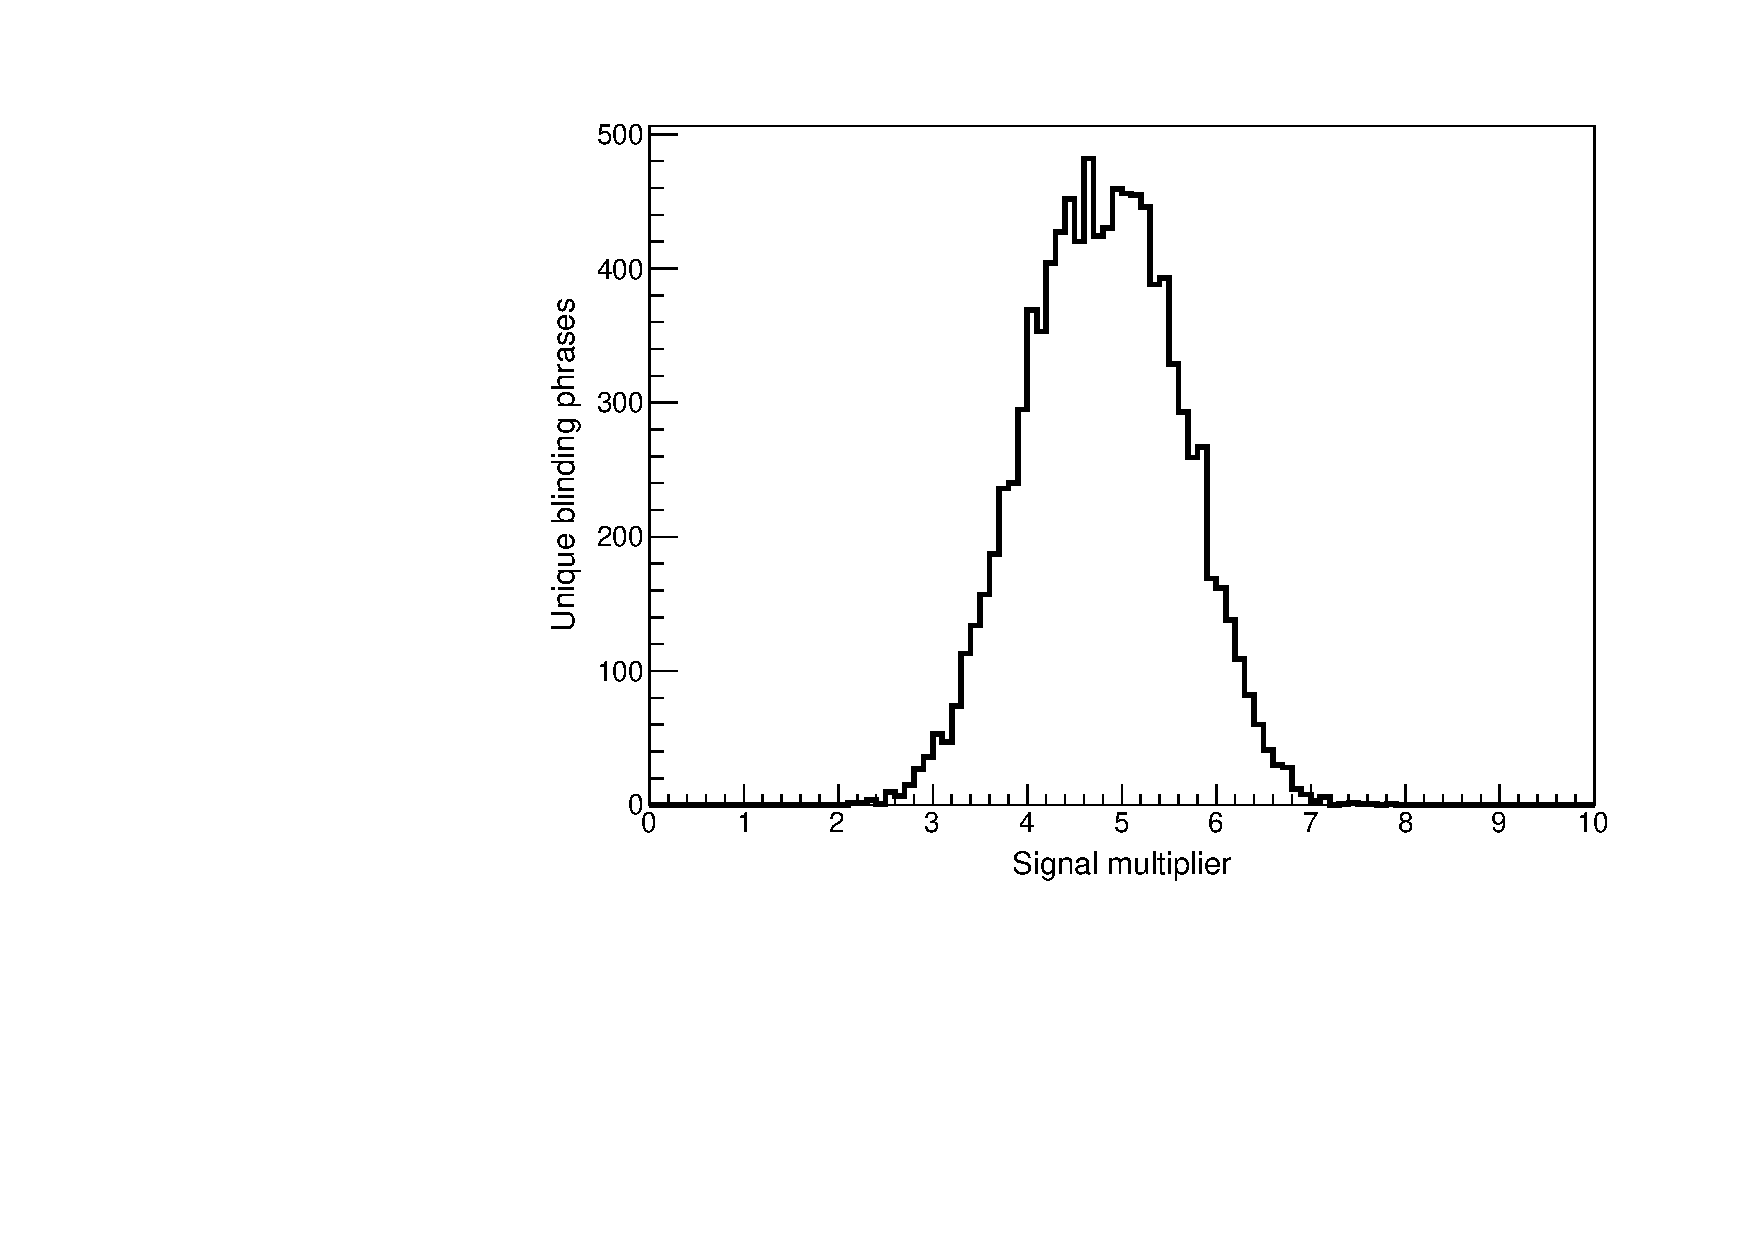
\includegraphics[trim={0 0 0 0},clip,width=.49\textwidth]{Images/Chapter6/Limits.pdf}\label{subfig:Limits}}
\subfloat[]{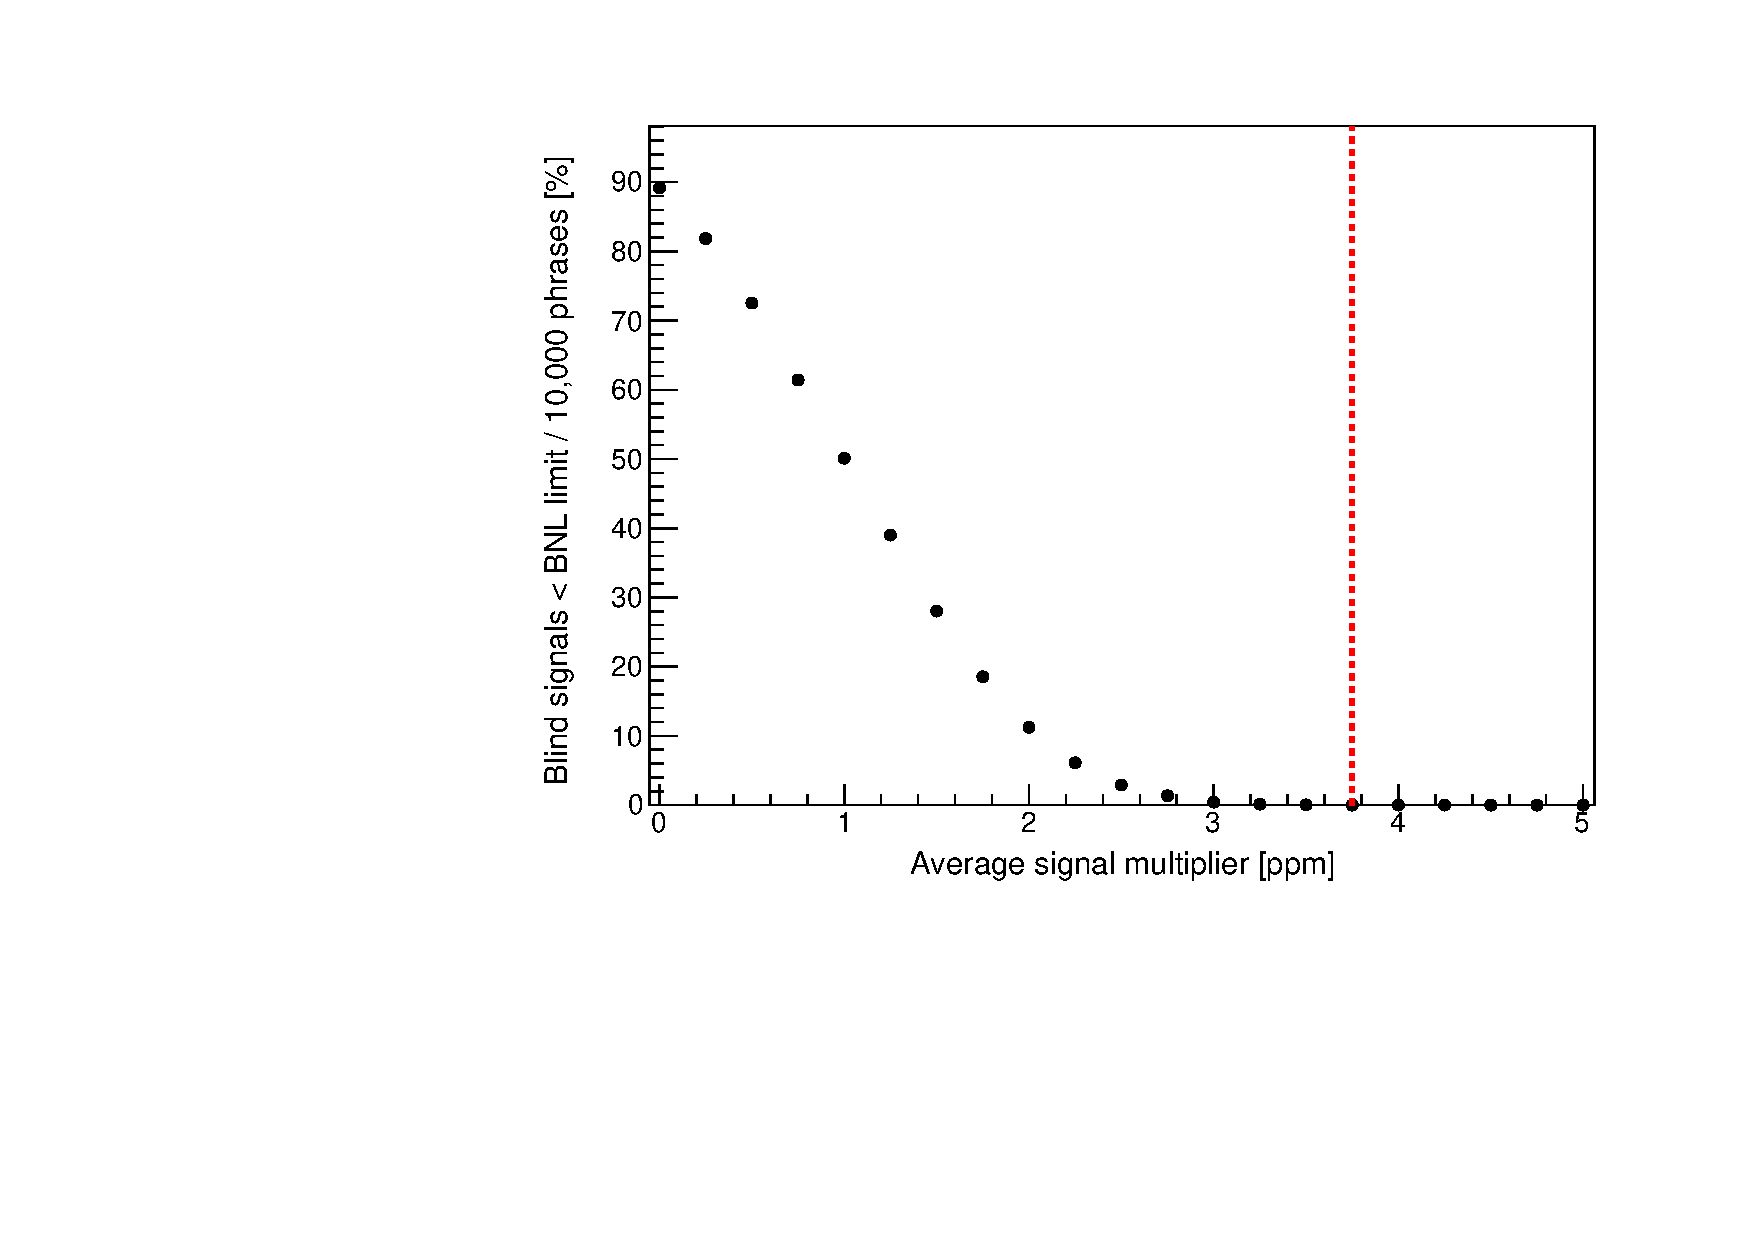
\includegraphics[trim={0 0 0 0},clip,width=.49\textwidth]{Images/Chapter6/RScan.pdf}\label{subfig:RScan}}
\caption{The EDM blind signal multipliers, showing: (a) the distribution of multipliers from 10,000 unique blinding phrases; (b) a scan over the average signal multiplier parameter, $G$, showing how any value of $G$ greater than 3.75 is sufficient to ensure that 100\% of the blind signal multipliers drawn from the aforementioned distribution are larger than the BNL EDM upper limit.}
\label{fig:Blinding}
\end{figure} 
%
\begin{figure}[t!]
\centering{}
\subfloat[Unblinded.]{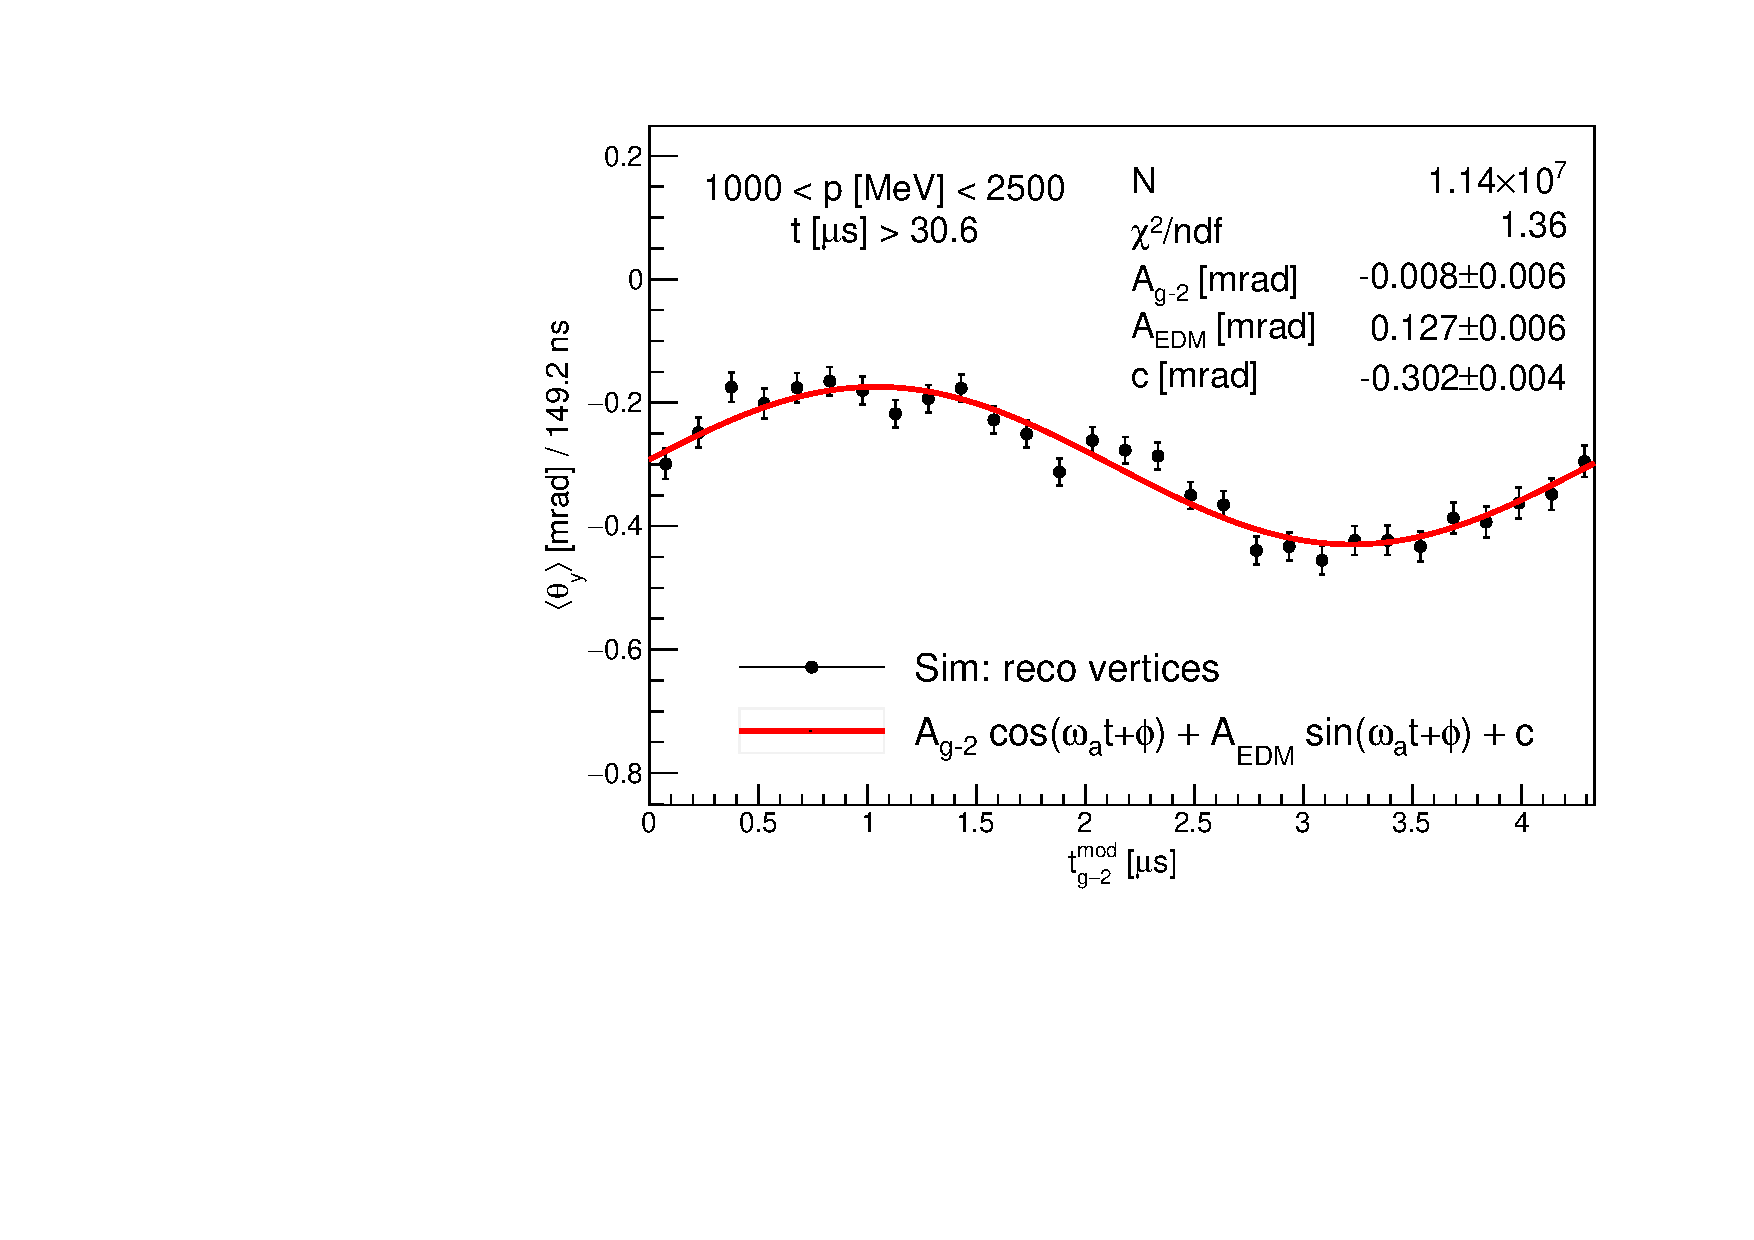
\includegraphics[trim={0 0 0 0},clip,width=.49\textwidth]{Images/Chapter6/S12S18_edmFit_thetaY_trackReco_WORLD_250MeV_BQ_noVertCorr_1.pdf}}
\subfloat[Blinded.]{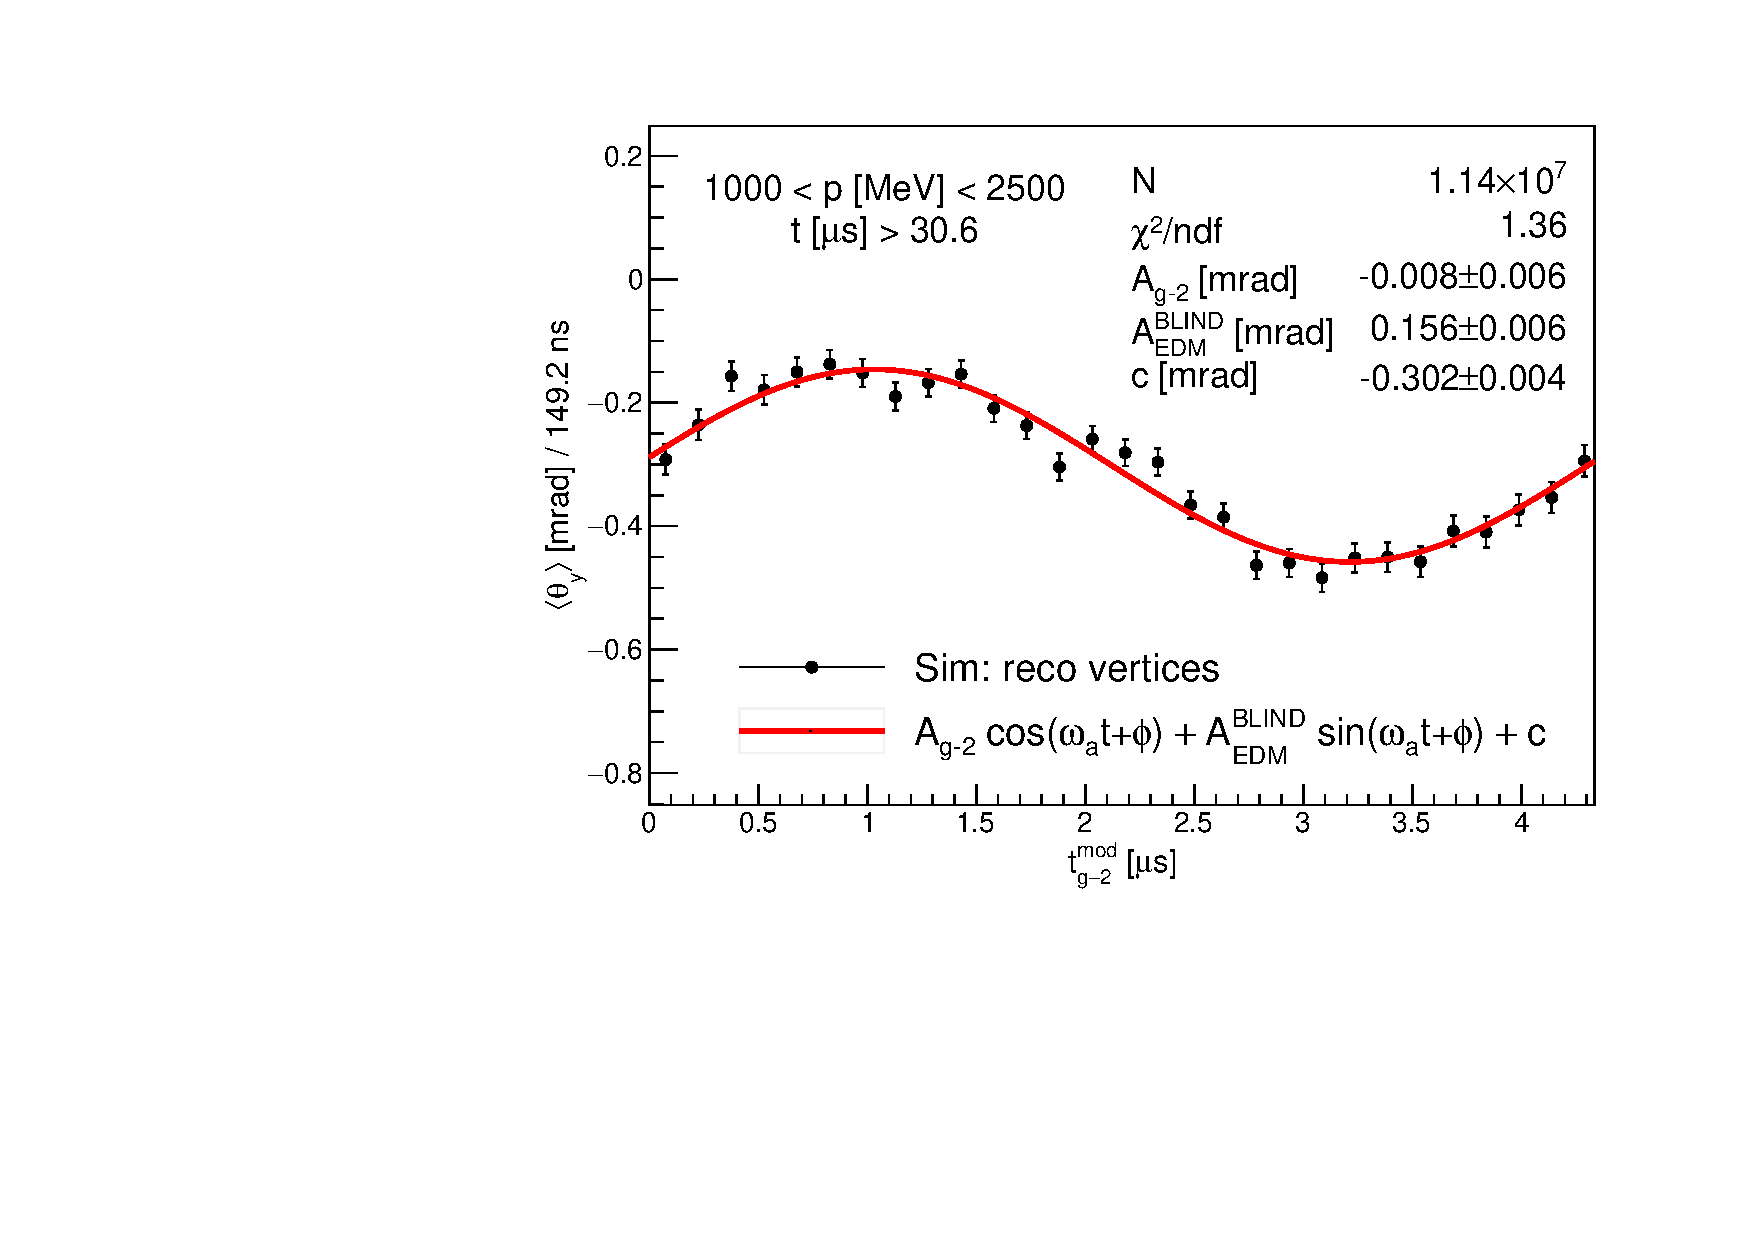
\includegraphics[trim={0 0 0 0},clip,width=.49\textwidth]{Images/Chapter6/S12S18_edmFit_thetaY_trackReco_WORLD_250MeV_BQ_noVertCorr_0.pdf}}
\caption{The EDM blinding applied to simulated track decay vertices with an injected muon EDM, demonstrating how the blinding procedure exclusively modifies the parameter $A_{\text{EDM}}$.}
\label{fig:BlindedSimFits}
\end{figure} 
%
\begin{equation}
  \theta_{y}^{\text{BLIND}}(t) = \theta_{y}(t) + A_{\text{EDM}}^{\text{BLIND}}(G, S)\cdot\sin(\omega_{a}t+\phi),
  \label{eqn:blinding}
\end{equation}
%
where $\phi$ is the anomalous precession phase. The constant $G$ is the average signal multiplier, or the average value of the flattened Gaussian distribution described above. This distribution is shown in Figure \ref{subfig:Limits}, for 10,000 unique blinding phrases, with chosen parameters of 0.25 for the width of the uniform section of the distribution, a width of 0.7 for the Gaussian tails, and a value of 4.81 for $G$. This value was selected to ensure that the injected signal is always larger than the BNL limit, as shown in Figure \ref{subfig:RScan}: with a red dashed line indicating the smallest value of $G$ where zero out of 10,000 trial blinding phrases resulted in a signal less than the BNL limit\footnote{The exact value of 4.81 was chosen for purely aesthetic reasons, besides being greater than 3.75, it being approximately equal to the transcendental number $(((i)^{i}){^i}){^i}$.}. 
%

A demonstration of the blinding applied to simulated track decay vertices with an known injected EDM signal, as detailed in the previous chapter, is shown in Figure \ref{fig:BlindedSimFits}. Critically, this demonstrates that the blinding increases the measured EDM angle without modifying the other fit parameters. Separate blinding phrases are used for simulation and data, and all Run-1 datasets share a common phrase.

% Sources of systematic uncertainty, as well statistical fluctuations, can produce results which appear intuitively sensible but are either not reproducible or a false positive.

\section{Fitting the vertical angle oscillation}\label{sec:Run1Fits}

In this section, blinded direct measurements of the EDM vertical angle oscillation in Run-1 are described. Both simultaneous and momentum-binned vertical angle oscillation fits, over a momentum range of 1000-2500 MeV, are presented. An example of underlying vertical angle distribution is shown, for Run-1a, in Figure \ref{fig:Run1aThetaY}, and widths of the vertical angle distributions for each Run-1 dataset are summarised in Table \ref{tbl:Run1aThetaY}.

\begin{figure}[h!]
\centering{}
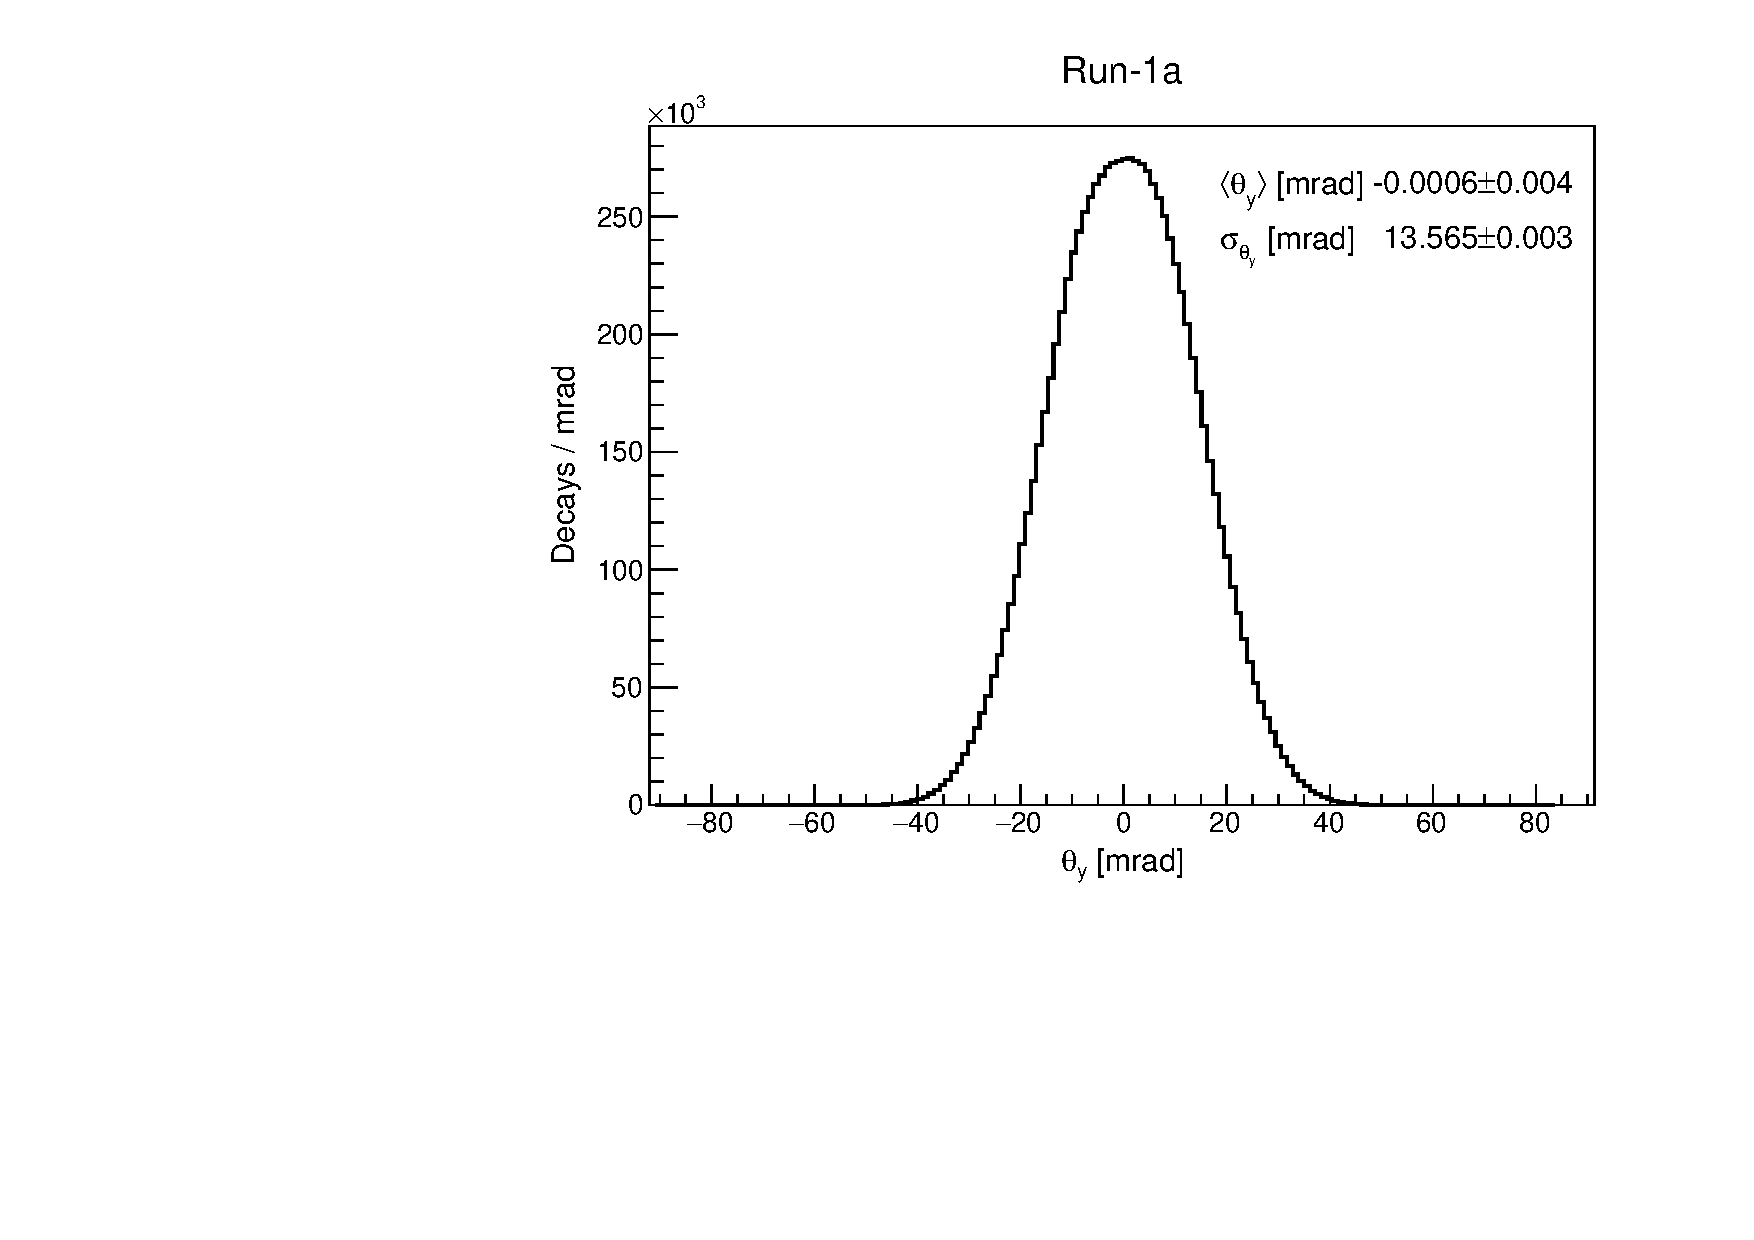
\includegraphics[trim={0 0 0 1cm},clip,width=.65\textwidth]{Images/Chapter6/ThetaY_Run-1a.pdf}
\caption{The distribution of $\theta_{y}$ for the Run-1a dataset (1000-2500 MeV).}
\label{fig:Run1aThetaY}
\end{figure} 

\begin{table}[h!]
\centering{}
\begin{tabular}{l|cccc}
\hline
\hline
Dataset & Run-1a & Run-1b & Run-1c & Run-1d \\ 
\hline
$\sigma_{\theta_{y}}$ [mrad] & $13.565\pm0.003$ & $13.598\pm0.003$ & $13.579\pm0.002$ & $13.635\pm0.002$ \\ 
\hline
\hline
\end{tabular}
\caption{The widths of the $\theta_{y}$ distributions in Run-1 (1000-2500 MeV).} 
\label{tbl:Run1aThetaY}
\end{table}

\clearpage

\subsection{Fits for the anomalous precession oscillation phase}

% The fit quality, as indicated by the $\chi^{2}/\text{NDF}$, is somewhat inferior in all cases except Run-1c, which might be attributed to the use of a simple five parameter fit function: in the $\omega_{a}$ analysis proper, additional parameters are included to absorb the various oscillations beam dynamics oscillations in the data.

As discussed in Chapters \ref{chap:2} and \ref{chap:5}, the first part of the EDM analysis procedure involves fitting the oscillation in the number of high-momentum tracks (the number oscillation) to determine the anomalous precession frequency phase, $\phi$. To this end, fits to the time-modulated number oscillation with the five parameter function, Equation \ref{eqn:FiveParFunc}, for each of the four Run-1 datasets are shown in Figure \ref{fig:Run1Phases}; the measured phases are reported in Table \ref{tbl:Run1Phases}. The impact of the number oscillation phase uncertainty on the EDM result is discussed in Section \ref{sec:PhaseUnc}. Additionally, and as will be expanded upon in Section \ref{sec:FitStartTimeScans}, the normal fit-start time of \SI{30.6}{\micro\second} ($7\times T_{g-2}$) was extended to \SI{52.4}{\micro\second} ($12\times T_{g-2}$) in the case of Run-1d. 



\begin{figure}[h!]
\centering{}
\subfloat[Run-1a.]{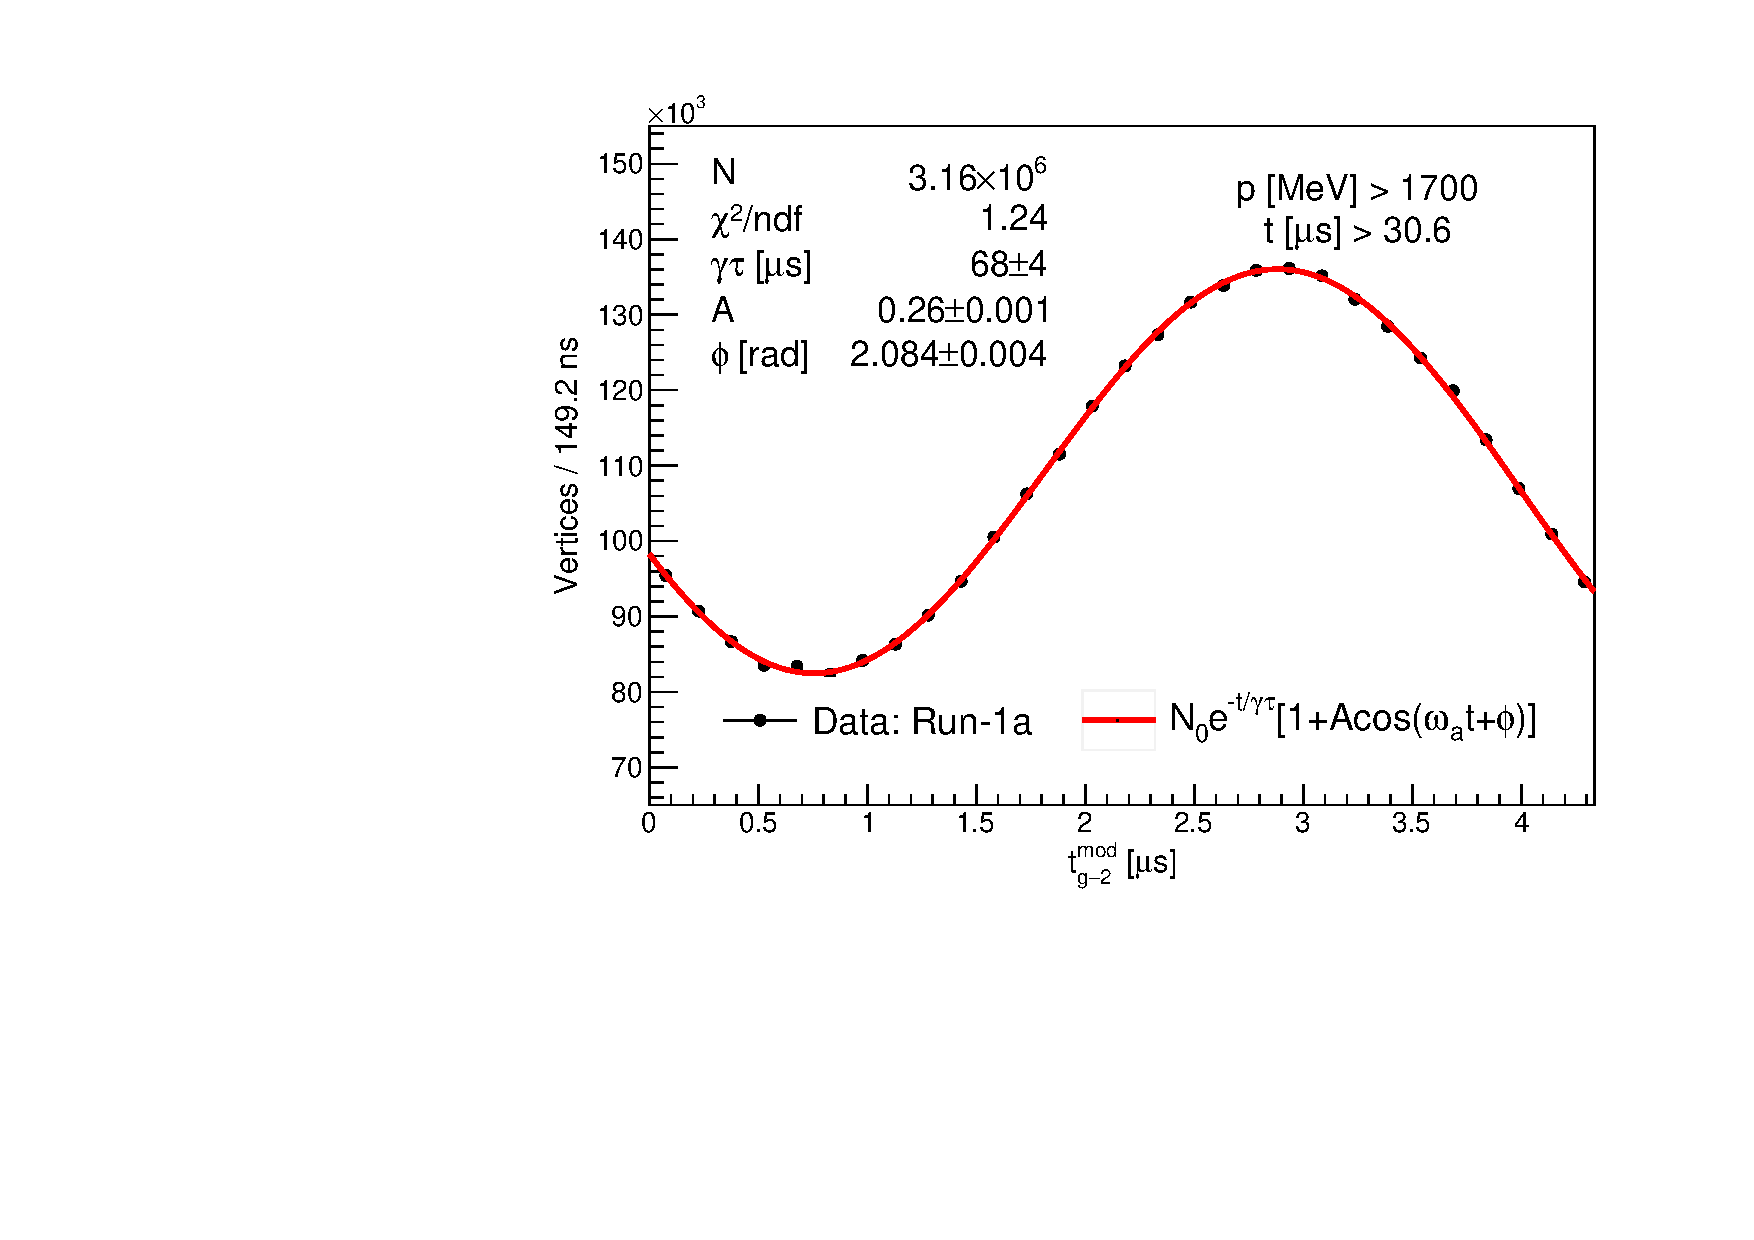
\includegraphics[trim={0 0 0 0},clip,width=.49\textwidth]{Images/Chapter6/fit_mod_wiggle_Run-1a_250MeV_1000_2500MeV_randomised_BQ.pdf}}
\subfloat[Run-1b.]{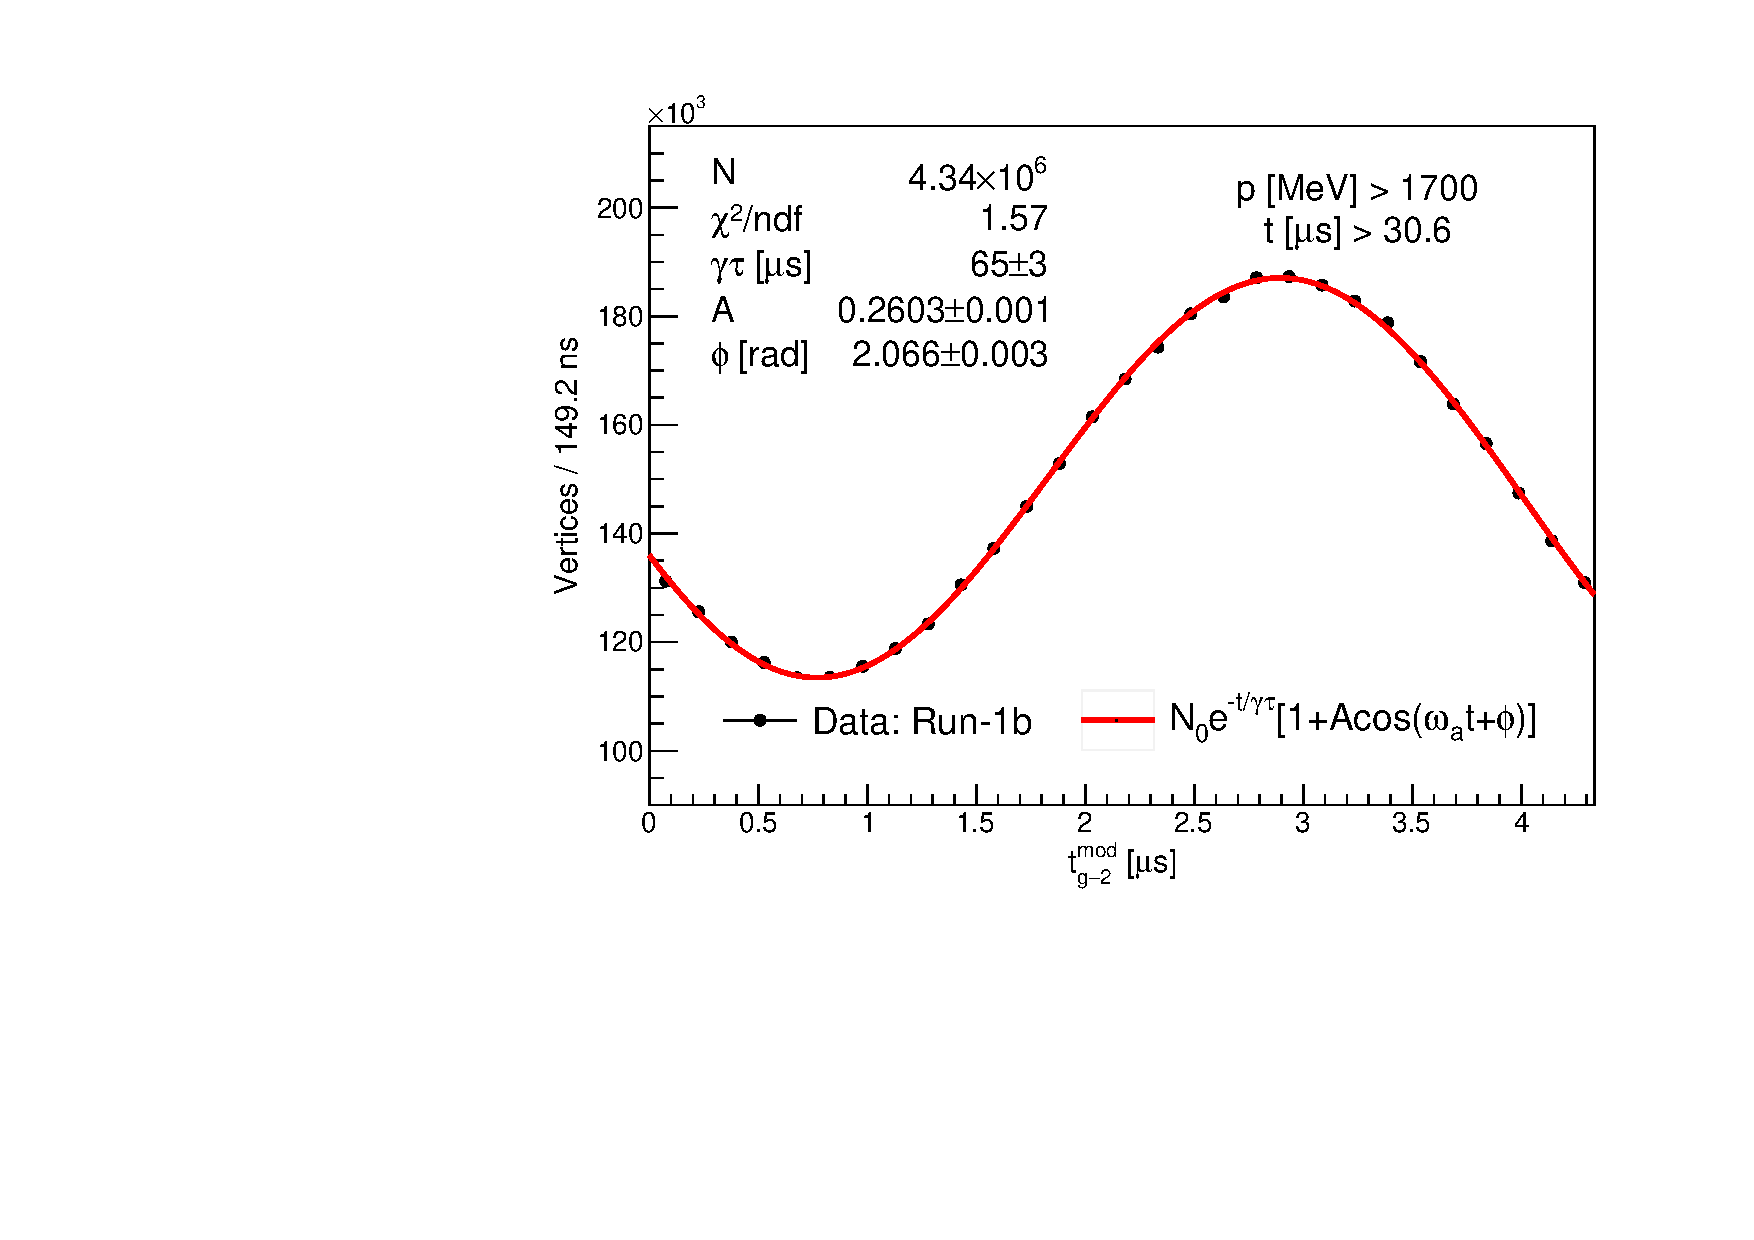
\includegraphics[trim={0 0 0 0},clip,width=.49\textwidth]{Images/Chapter6/fit_mod_wiggle_Run-1b_250MeV_1000_2500MeV_randomised_BQ.pdf}}
\hfill
\subfloat[Run-1c.]{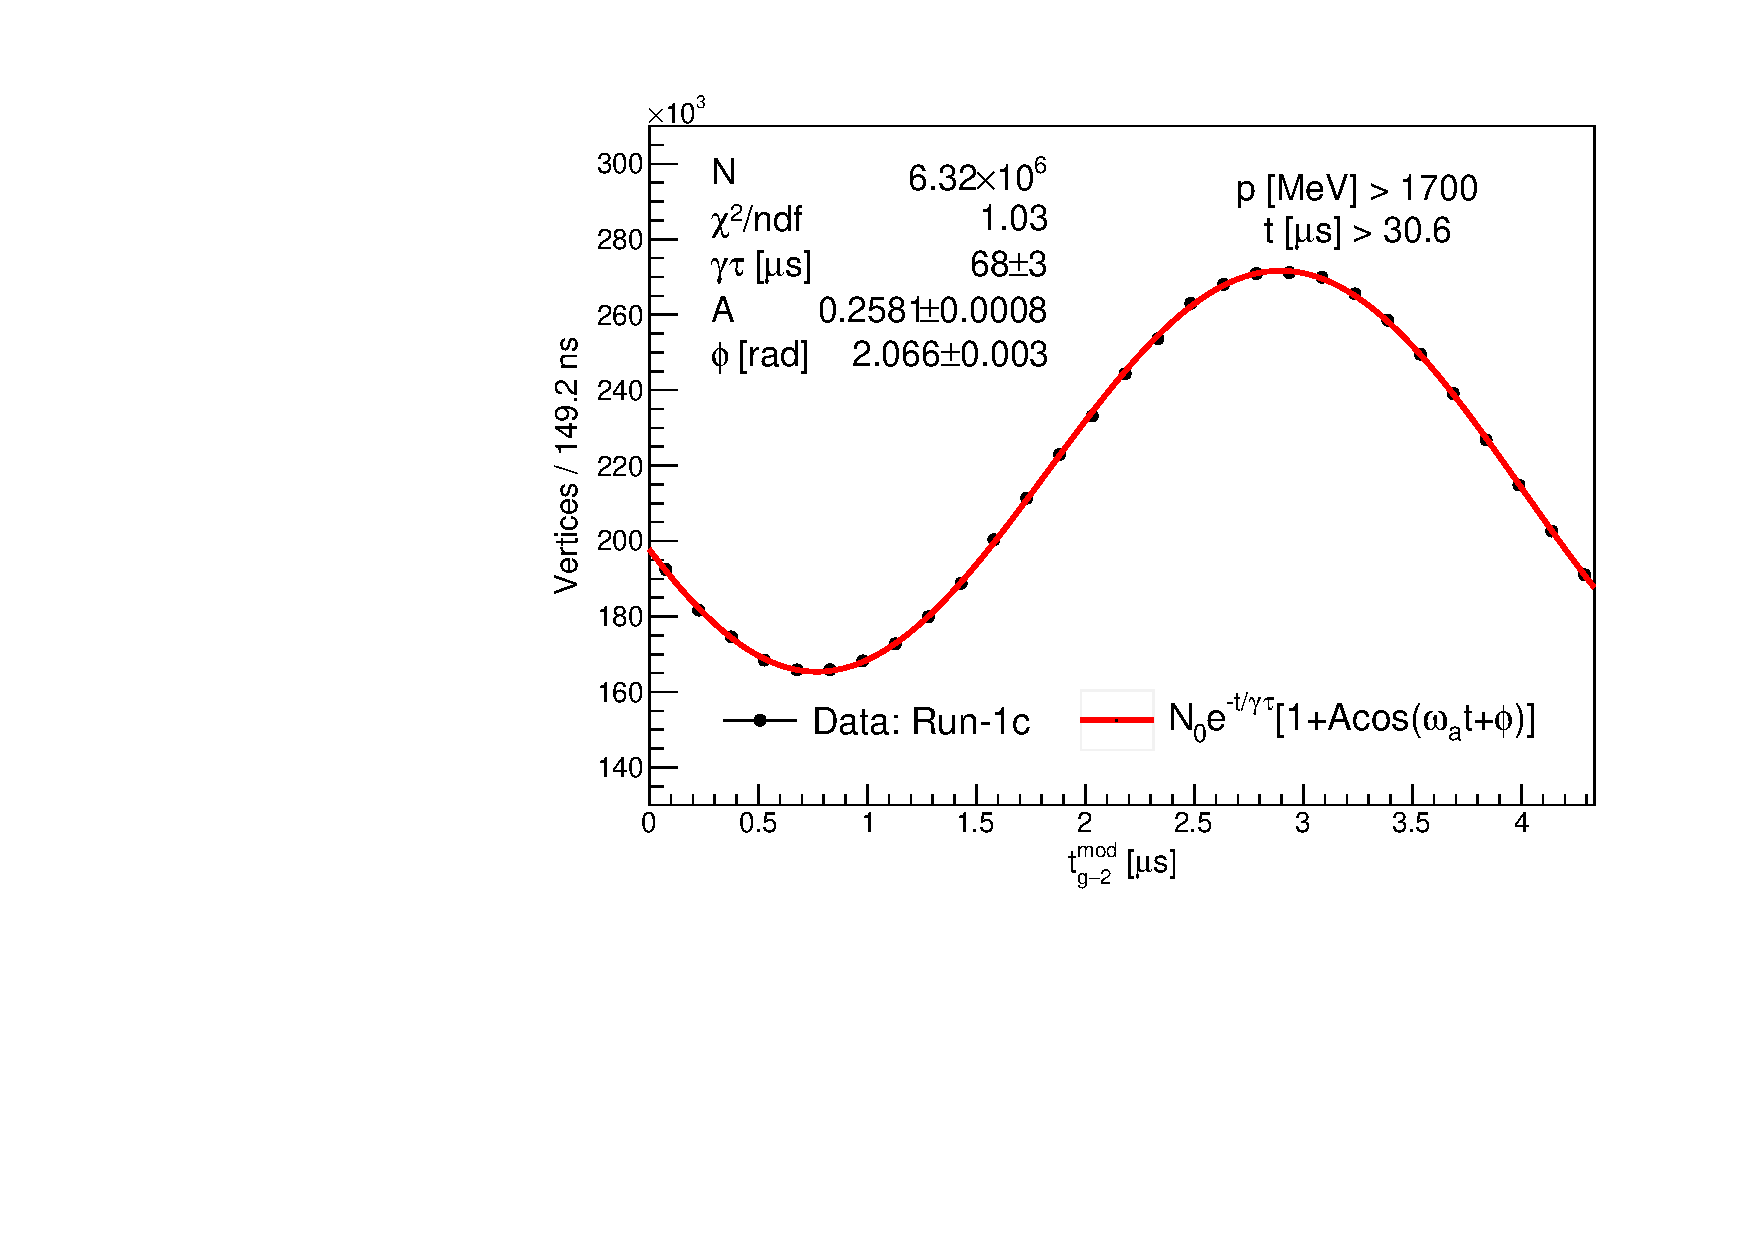
\includegraphics[trim={0 0 0 0},clip,width=.49\textwidth]{Images/Chapter6/fit_mod_wiggle_Run-1c_250MeV_1000_2500MeV_randomised_BQ.pdf}}
\subfloat[Run-1d.]{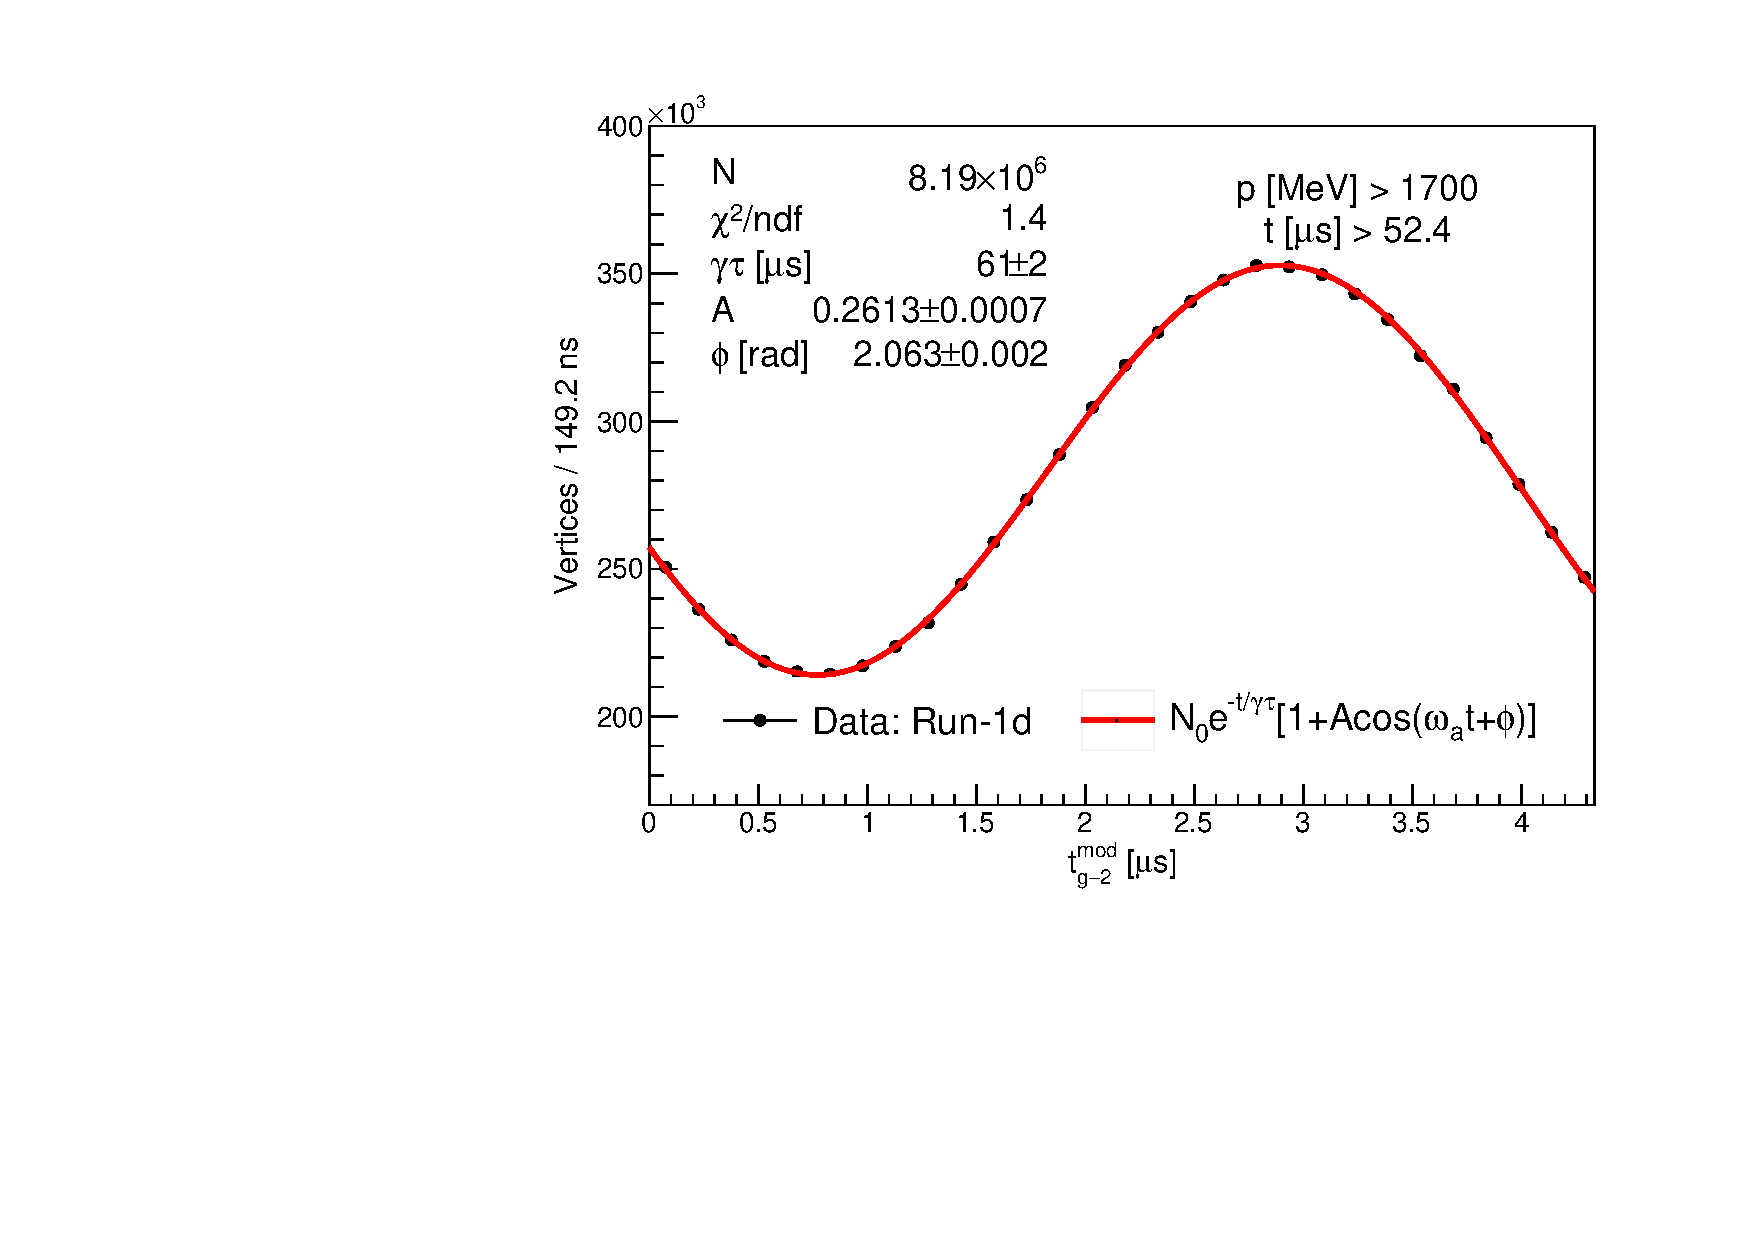
\includegraphics[trim={0 0 0 0},clip,width=.49\textwidth]{Images/Chapter6/fit_mod_wiggle_Run-1d_250MeV_1000_2500MeV_50usStartTime_randomised_BQ.pdf}}
\caption{Fits for the anomalous precession oscillation phase, $\phi$, in Run-1.}
\label{fig:Run1Phases}
\end{figure} 

\begin{table}[h!]
\centering{}
\begin{tabular}{l|cccc}
\hline
\hline
Dataset & Run-1a & Run-1b & Run-1c & Run-1d \\
\hline
$\phi$ [rad] & $2.084\pm0.004$ & $2.066\pm0.003$ & $2.066\pm0.003$ & $2.063\pm0.002$ \\ 
\hline
\hline
\end{tabular}
\caption{The measured anomalous precession oscillation phases, $\phi$, in Run-1.} 
\label{tbl:Run1Phases}
\end{table}

\subsection{Simultaneous vertical angle oscillation fits}

With the phase measured for each dataset, fits to the average vertical angle oscillation, $\langle \theta_{y} \rangle (t)$, in each dataset were initially performed over a wide range of momentum: 1000-2500 MeV, as discussed in Chapter \ref{chap:5}. These fits do not constitute a part of the EDM analysis proper, which utilises a momentum-binned approach, but fitting momentum bins simultaneously still has value as a cross-check of the main result. 

\begin{figure}[h!]
\centering{}
\subfloat[Run-1a.]{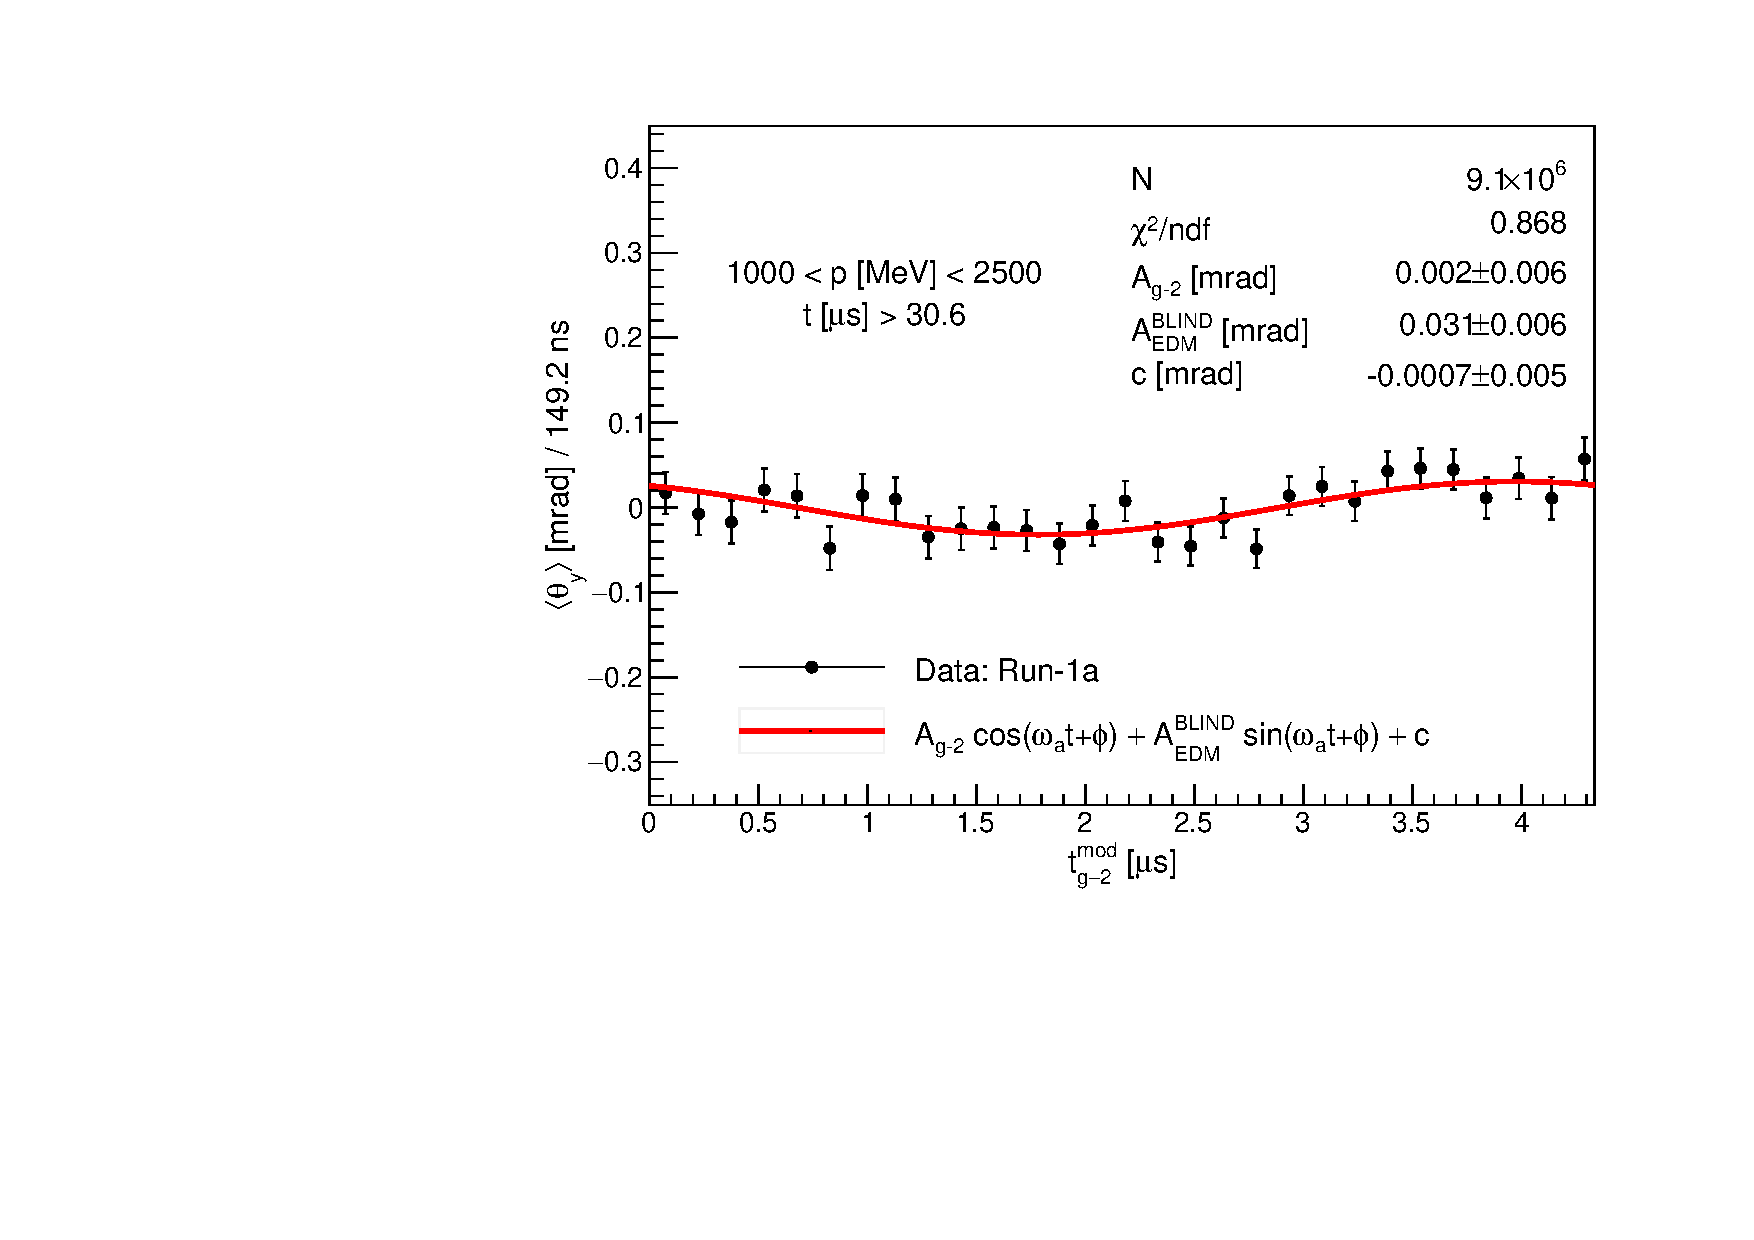
\includegraphics[trim={0 0 0 0},clip,width=.49\textwidth]{Images/Chapter6/S12S18_edmFit_Run-1a_250MeV_1000_2500MeV_randomised_BQ.pdf}}
\subfloat[Run-1b.]{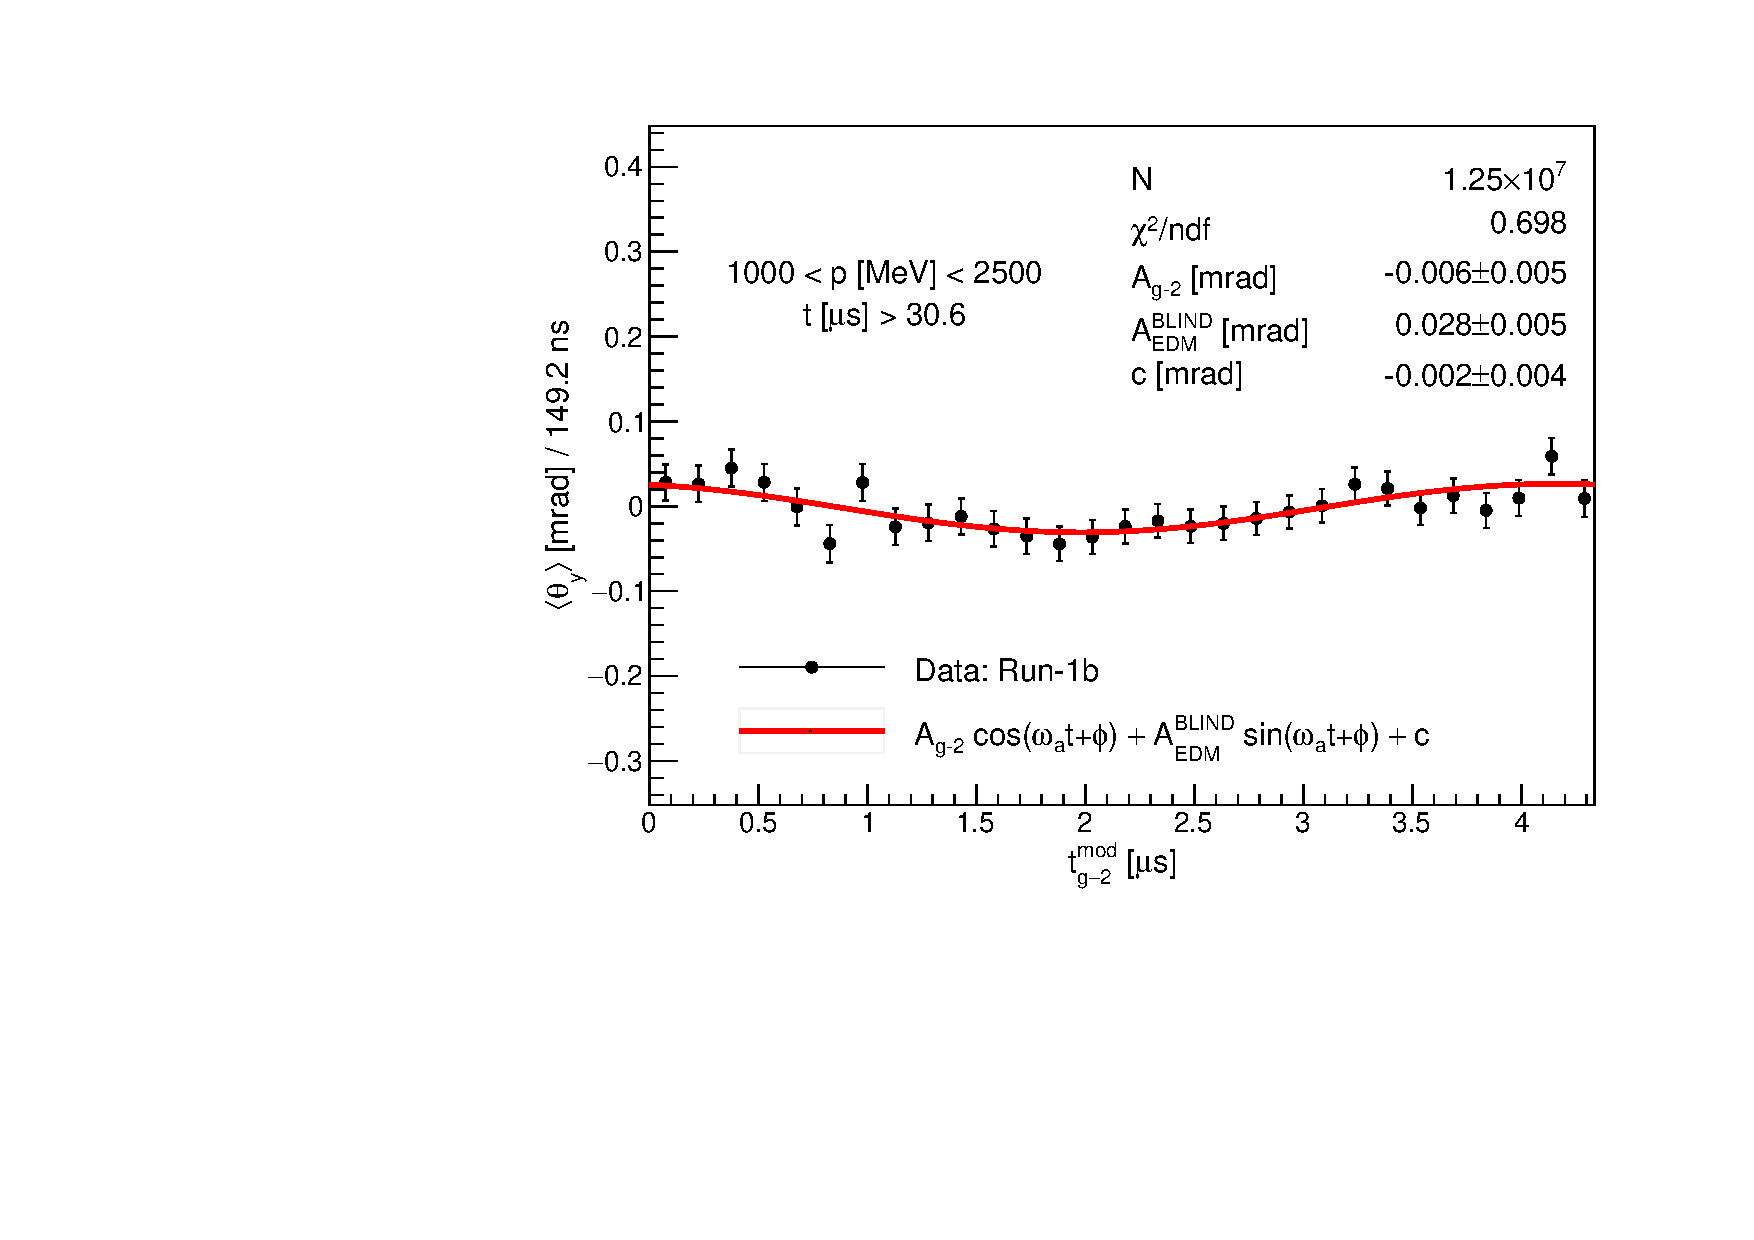
\includegraphics[trim={0 0 0 0},clip,width=.49\textwidth]{Images/Chapter6/S12S18_edmFit_Run-1b_250MeV_1000_2500MeV_randomised_BQ.pdf}}
\hfill
\subfloat[Run-1c.]{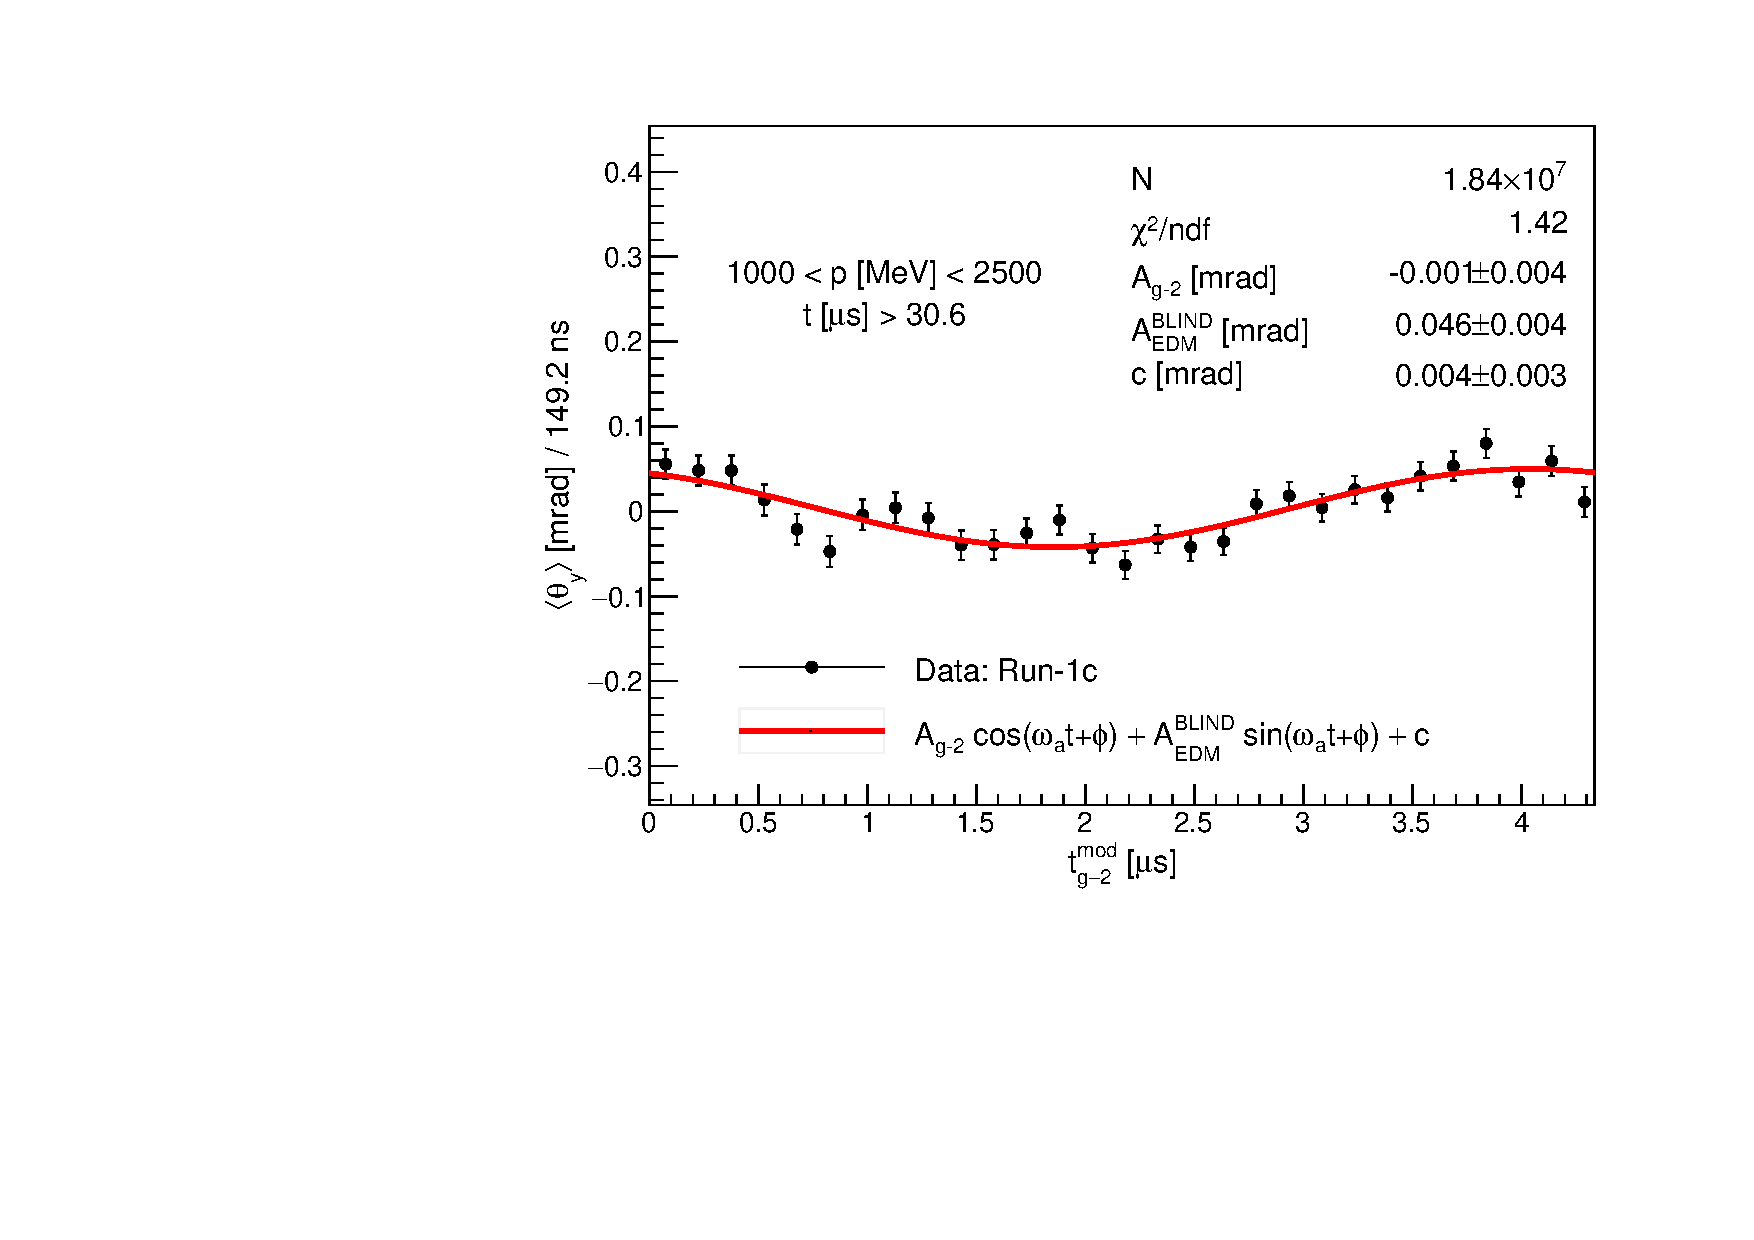
\includegraphics[trim={0 0 0 0},clip,width=.49\textwidth]{Images/Chapter6/S12S18_edmFit_Run-1c_250MeV_1000_2500MeV_randomised_BQ.pdf}}
\subfloat[Run-1d.]{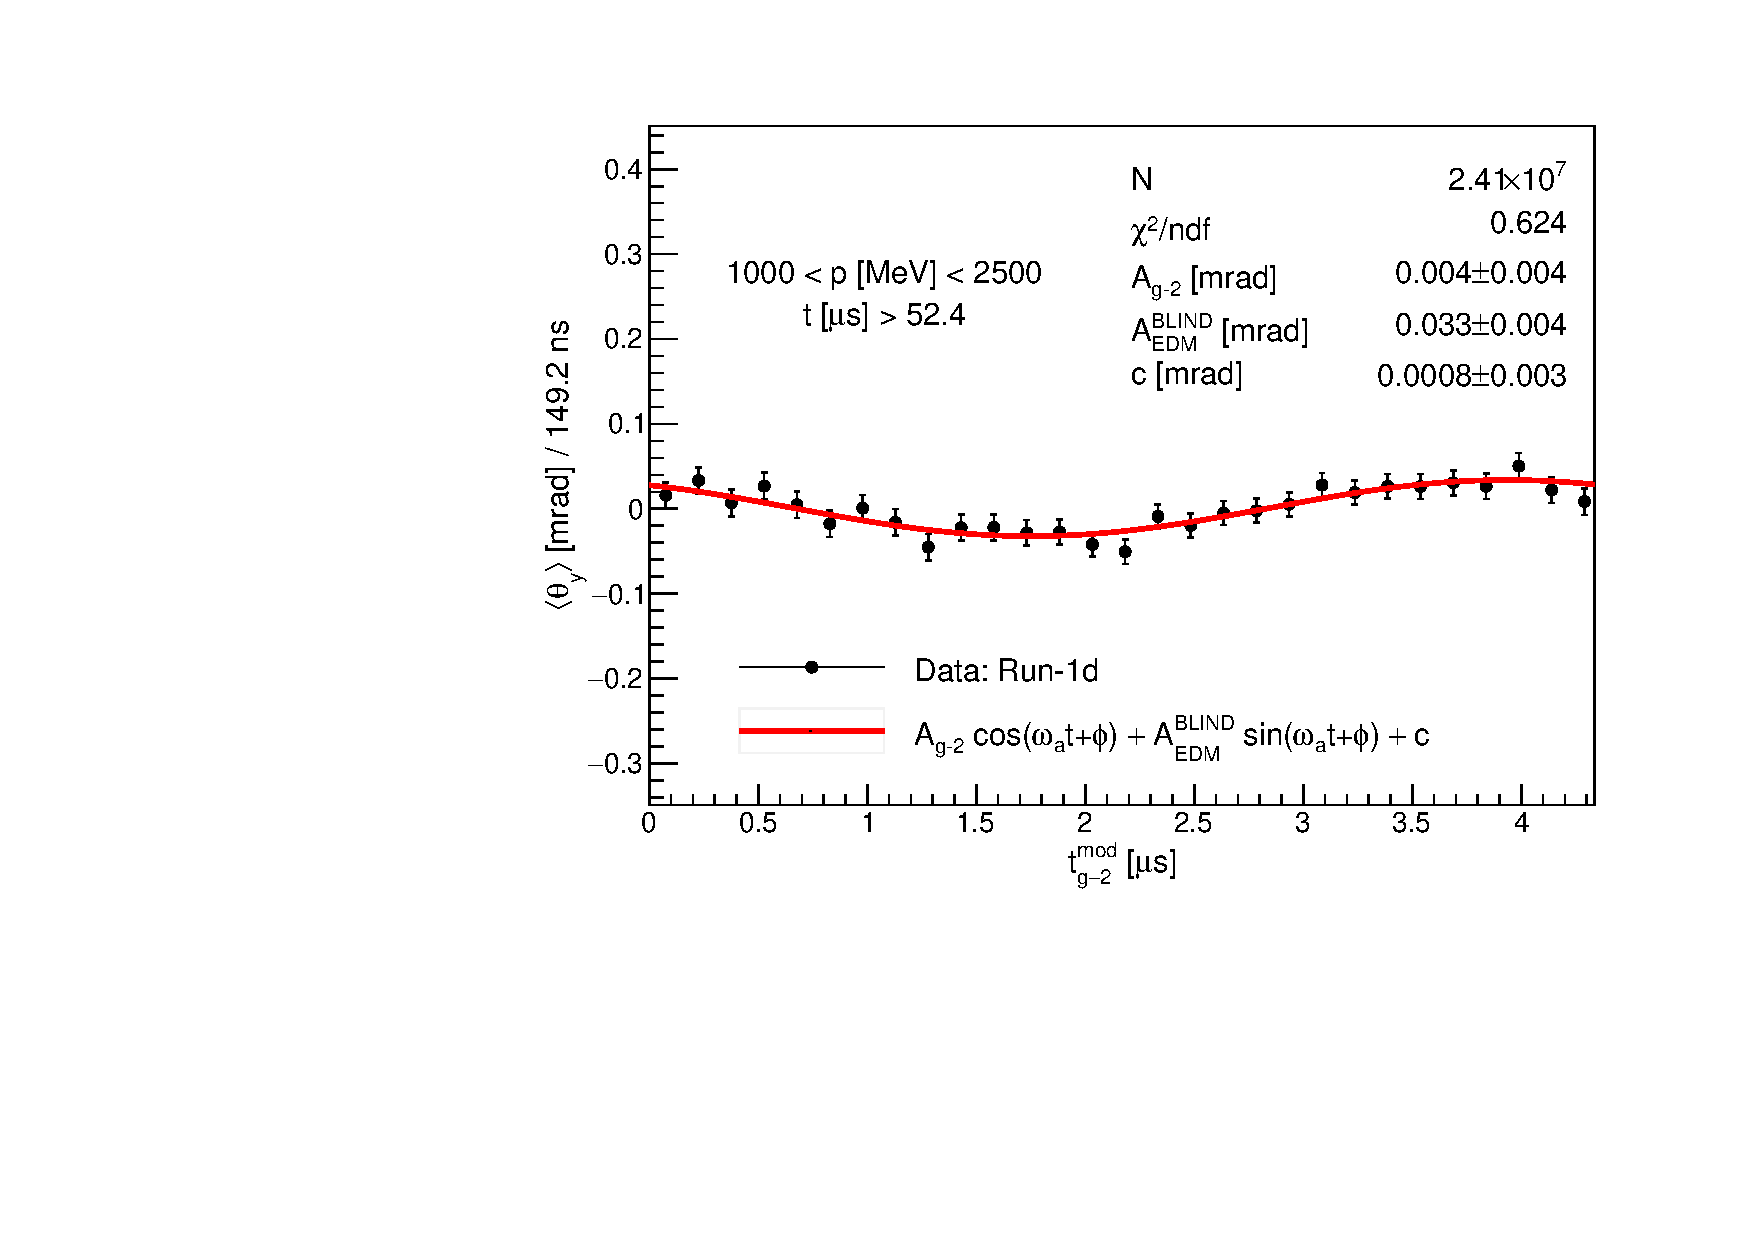
\includegraphics[trim={0 0 0 0},clip,width=.49\textwidth]{Images/Chapter6/S12S18_edmFit_Run-1d_250MeV_1000_2500MeV_50usStartTime_randomised_BQ.pdf}}
\caption{Blinded vertical angle oscillation fits. Tracker stations are combined.}
\label{fig:Run1BasicFits}
\end{figure} 

\begin{table}[h!]
\centering{}
\begin{tabular}{l|ccc}
\hline
\hline
Dataset & $A_{\text{EDM}}^{\text{BLIND}}$ [mrad] & $\delta^{\text{BLIND}}$ [mrad] \\ %& $d_{\mu}^{\text{BLIND}}$ [$\times10^{18}$ $e\cdot$cm] \\
\hline
Run-1a  & $0.031\pm0.006$ & $0.41\pm0.08$ \\%& $1.3\pm0.3$ \\ 
Run-1b  & $0.028\pm0.005$ & $0.37\pm0.07$ \\ %& $1.2\pm0.2$ \\
Run-1c  & $0.046\pm0.004$ & $0.61\pm0.06$ \\ % & $1.9\pm0.2$ \\
Run-1d  & $0.033\pm0.004$ & $0.44\pm0.06$ \\ %& $1.4\pm0.2$ \\ 
\hline
\hline
\end{tabular}
\caption{Blinded vertical angle oscillation fit results. Tracker stations are combined.} 
\label{tbl:Run1BasicFits}
\end{table}

\clearpage

These simultaneous fits, with tracker stations 12 and 18 combined, are shown in Figure \ref{fig:Run1BasicFits}. The results are reported in Table \ref{tbl:Run1BasicFits}, which includes a blind laboratory frame tilt angle, $\delta^{\text{BLIND}}$. This is calculated by Equation \ref{eqn:DilutionFunction2}, using the constant dilution factor of $d_{\text{EDM}}=0.075\pm0.004$ for this momentum range, from Table \ref{tbl:BasicSimFits}. It is important to note that the $\delta^{\text{BLIND}}$ values presented in this section have no radial magnetic field correction applied, and all uncertainties are statistical. The fit $\chi^{2}/\text{NDF}$ values are $<$1 with the exception of Run-1c, which is typically indicates an overestimation of the uncertainty on $\langle\theta_{y}\rangle$ per time bin. However, the uncertainties in question are purely statistical and are therefore well motivated. 



% Fits and tables of results for individual stations can be found in Appendix \ref{app:Run1AdditionalTablesAndFigures}. 

% As will be expanded upon in \myworries{Section XX}, various corrections were applied prior to fitting, including the removal of frequencies at a time period less than $T_{g-2}$ and the correction of average vertical angle in momentum and time. Only quality cut passing extrapolated track vertices were used. \myworries{WE NEED TO DESCRIBE WHAT THESE ARE!}



\subsection{Momentum-binned vertical angle oscillation fits}

As introduced in Chapter \ref{chap:5} Section \ref{sec:FittingThetaYSim}, the muon EDM search described in this thesis employs a momentum-binned approach: where fits to vertical angle oscillation are performed in momentum intervals, in an effort to improve the accuracy of the dilution correction, and to minimise momentum-dependant variations in the average vertical angle. 

% \begin{figure}[b!]
% \centering{}
% \subfloat[Station 12.]{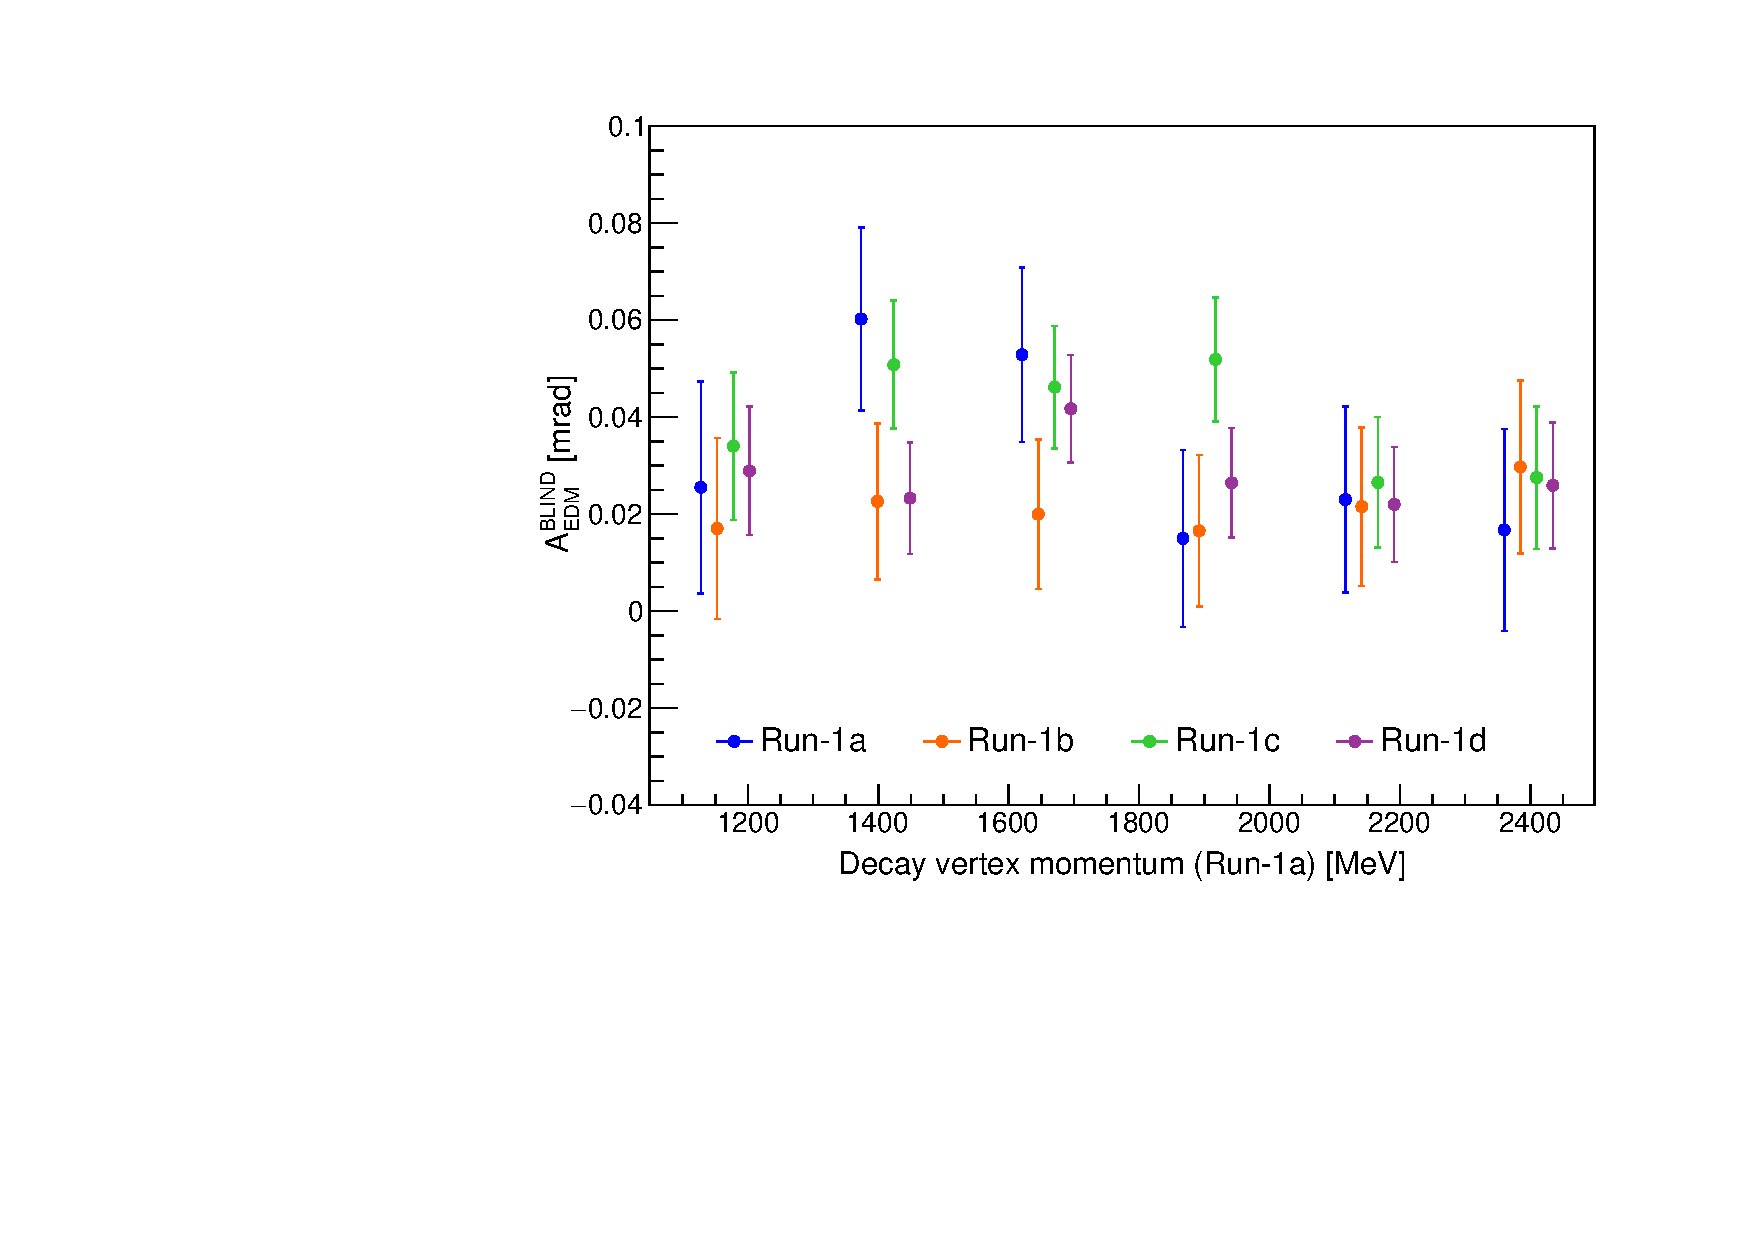
\includegraphics[trim={0 0 0 0},clip,width=.49\textwidth]{Images/Chapter6/S12_AEDM_vs_p_overlay_1000_2500.pdf}}
% \subfloat[Station 18.]{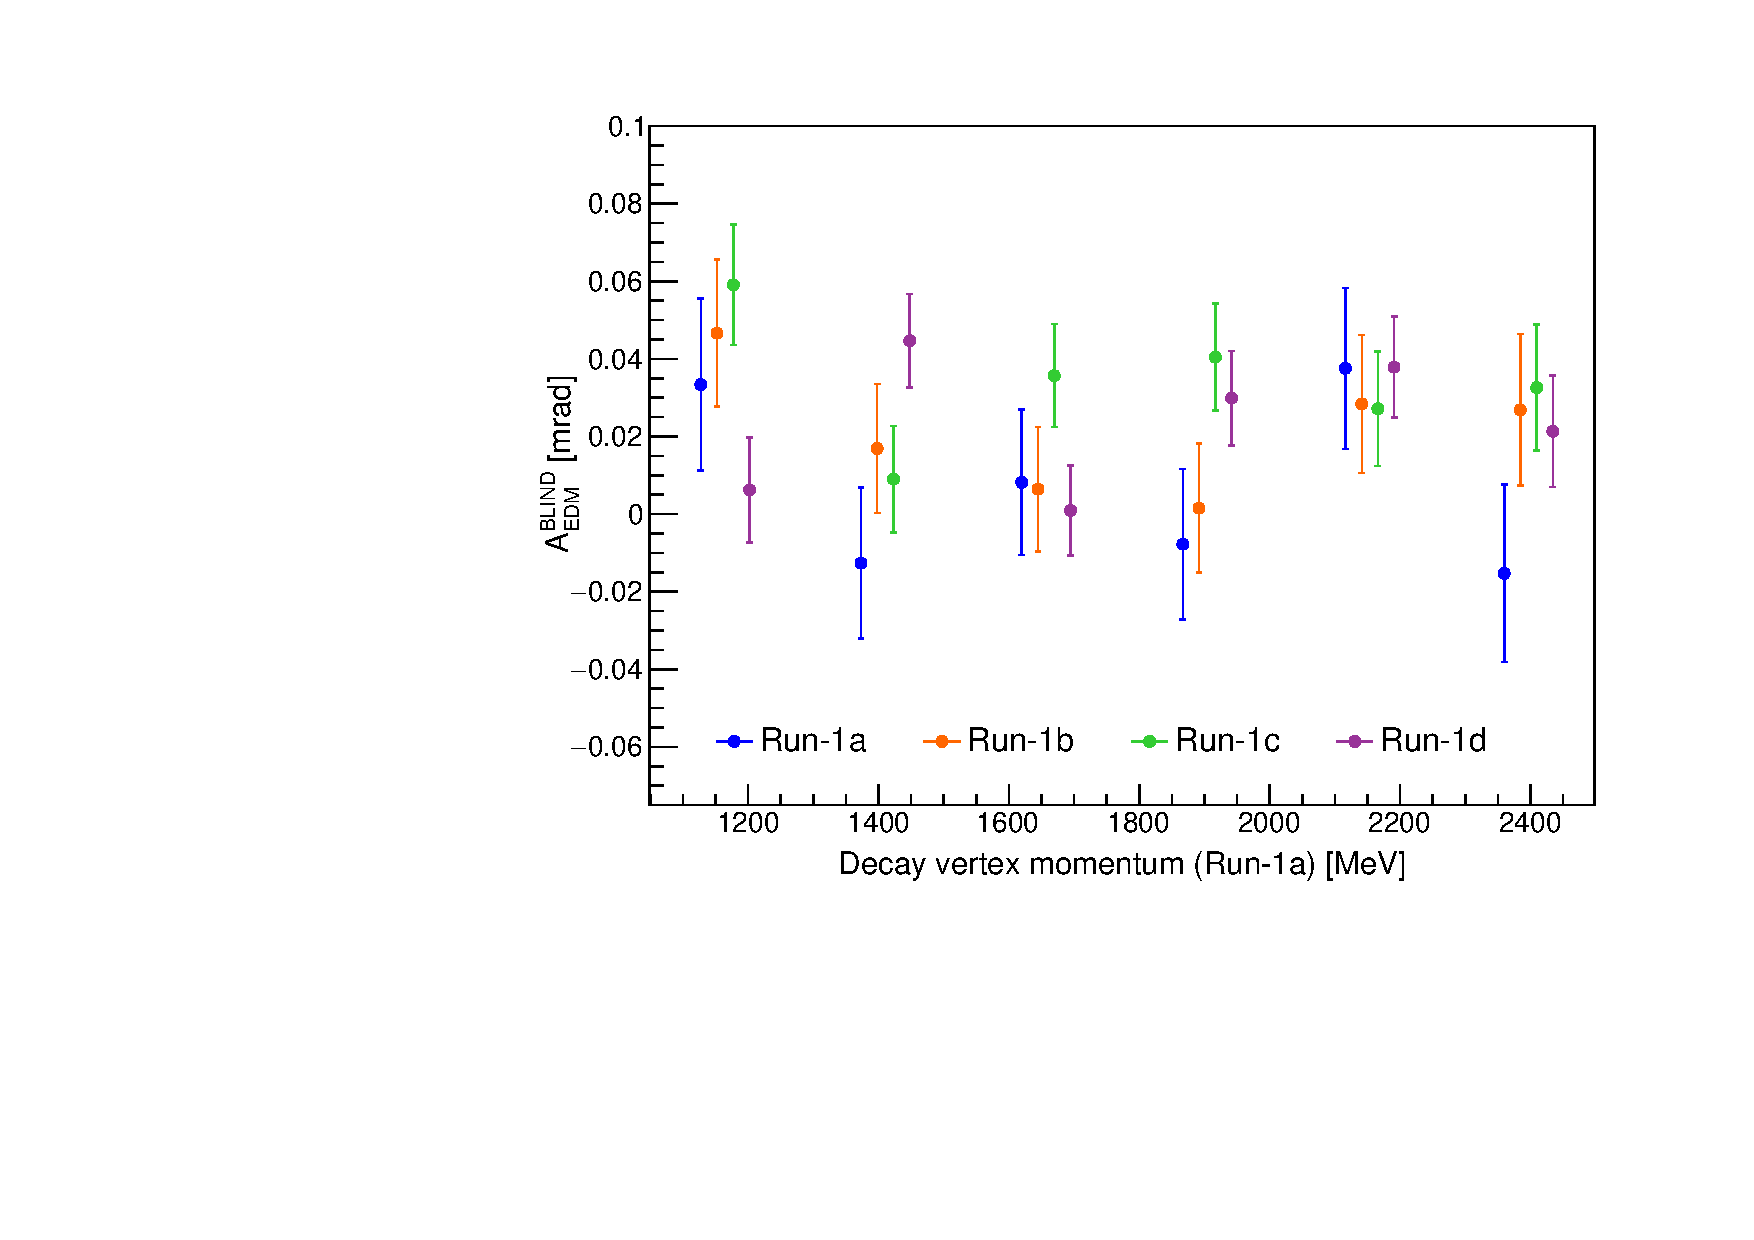
\includegraphics[trim={0 0 0 0},clip,width=.49\textwidth]{Images/Chapter6/S18_AEDM_vs_p_overlay_1000_2500.pdf}}\hfill
% \subfloat[Combined.]{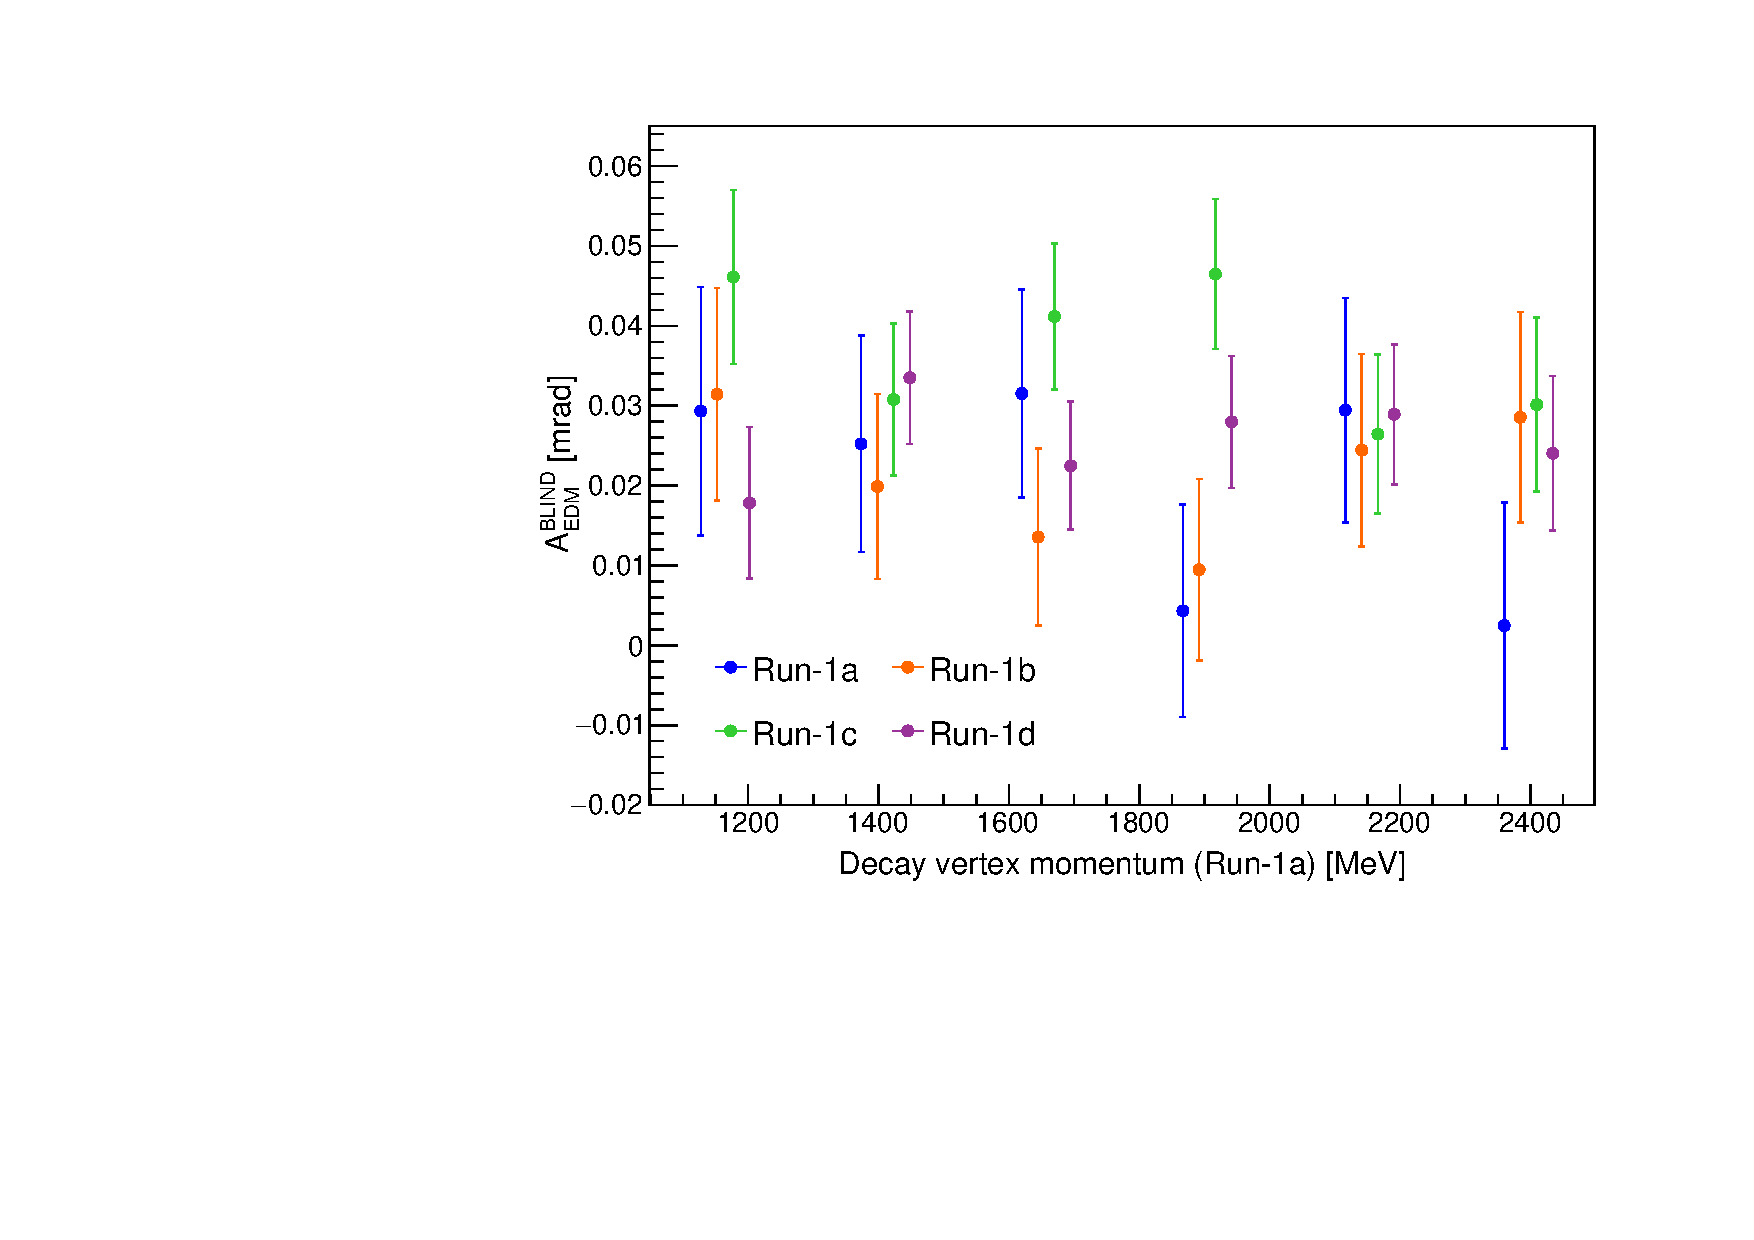
\includegraphics[trim={0 0 0 0},clip,width=0.69\textwidth]{Images/Chapter6/S12S18_AEDM_vs_p_overlay_1000_2500.pdf}}
% \caption{$A_{\text{EDM}}^{\text{BLIND}}$ per momentum bin for each Run-1 dataset. }
% \label{fig:Run1AEDM}
% \end{figure} 

\begin{figure}[b!]
\centering{}
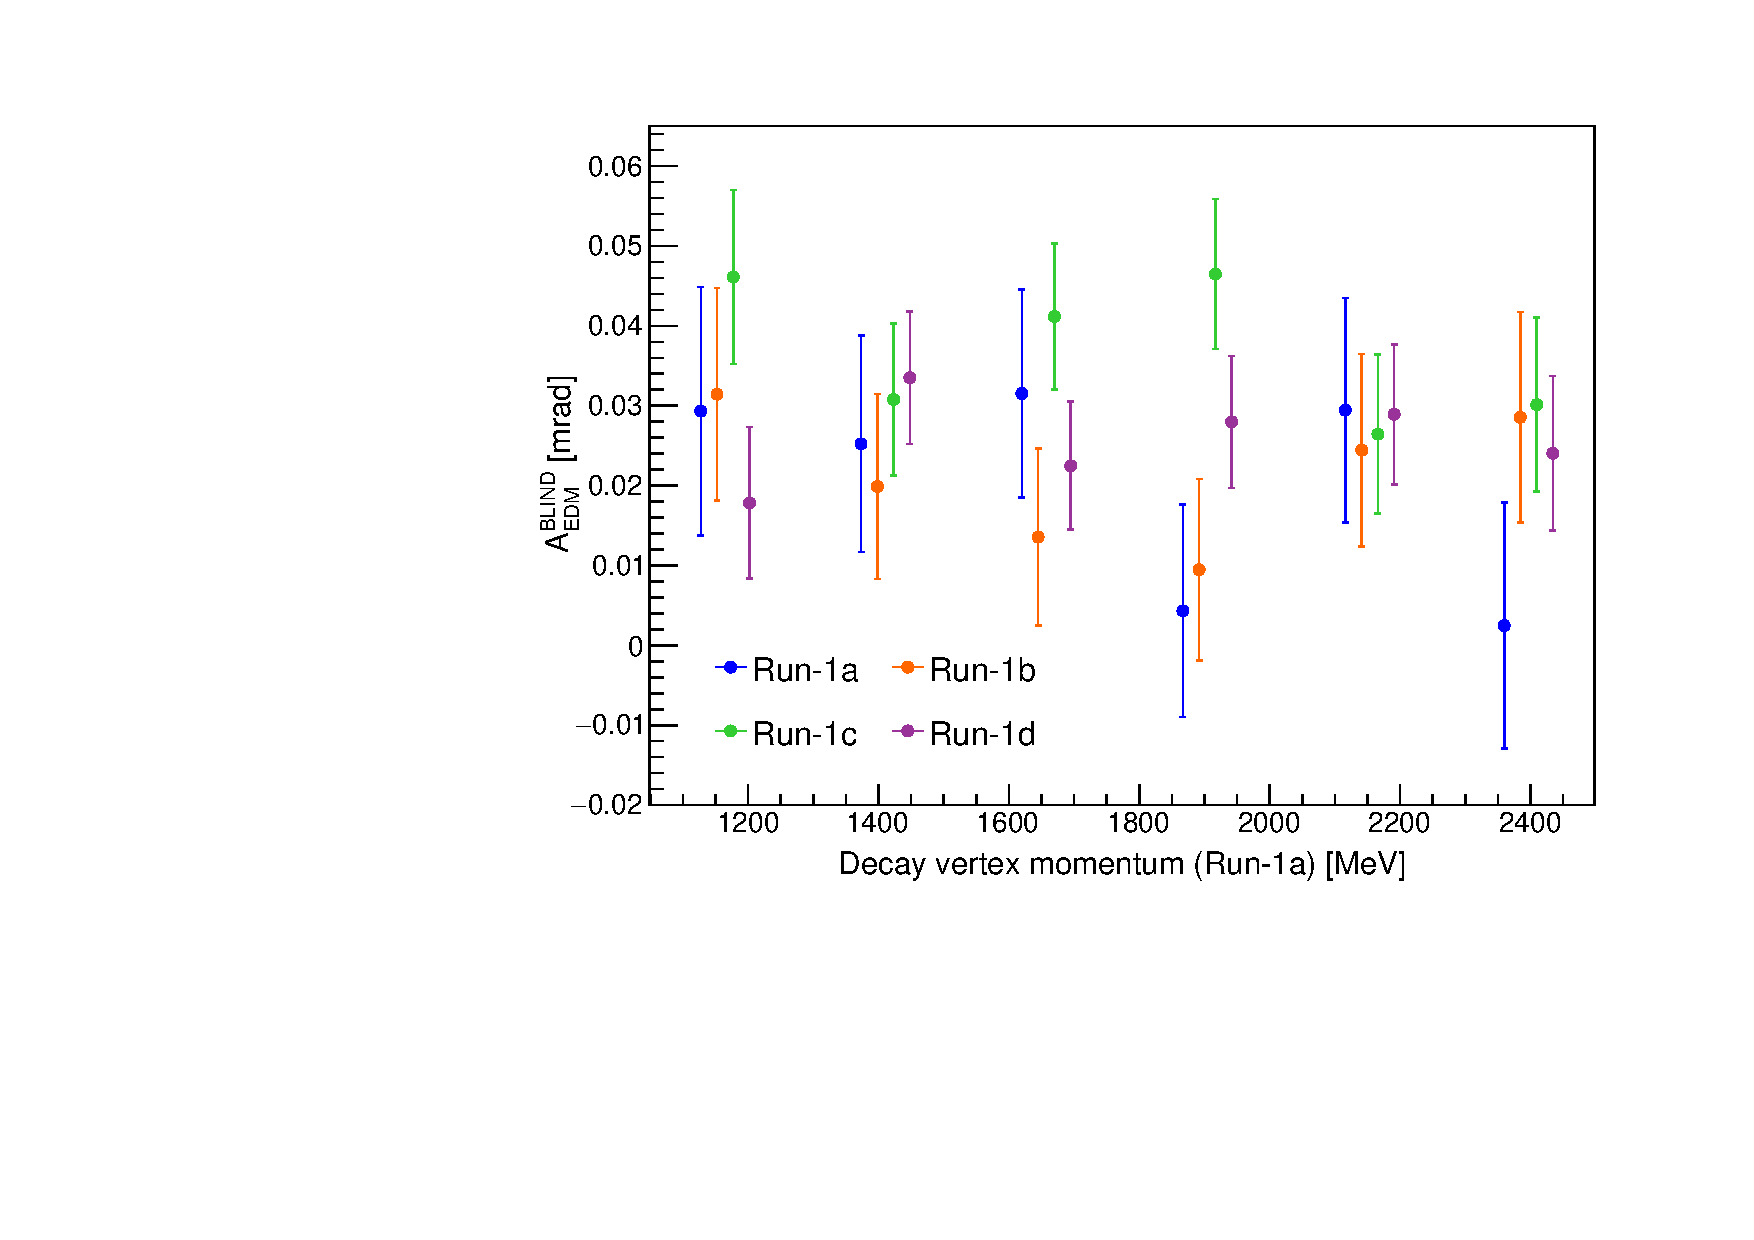
\includegraphics[trim={0 0 0 0},clip,width=0.69\textwidth]{Images/Chapter6/S12S18_AEDM_vs_p_overlay_1000_2500.pdf}
\caption{$A_{\text{EDM}}^{\text{BLIND}}$ per momentum bin for each Run-1 dataset. Tracker stations are combined.}
\label{fig:Run1AEDM}
\end{figure} 

Momentum-binned fits over a range of 1000-2500 MeV, in intervals of 250 MeV, are shown for each Run-1 dataset in Figures \ref{fig:Run1aMomBinnedFits}, \ref{fig:Run1bMomBinnedFits}, \ref{fig:Run1cMomBinnedFits}, and \ref{fig:Run1dMomBinnedFits}; where tracker stations are combined in each case. The measured values of $A_{\text{EDM}}^{\text{BLIND}}$ per momentum bin are presented for each dataset in Figure \ref{fig:Run1AEDM}. Additionally, the corresponding fit $\chi^{2}/\text{NDF}$ values are shown in Figure \ref{fig:Chi2Run1MomBinnedFits}, with a zeroth order polynomial fit giving an estimate of the average, $\langle \chi^{2}/\text{NDF} \rangle$, over the full range of momentum. These averages are consistent with one to within a maximum of $1.5\sigma$ (in the case of Run-1b), indicating good quality fits. 

\begin{figure}[t!]
\centering{}
\subfloat[Run-1a.]{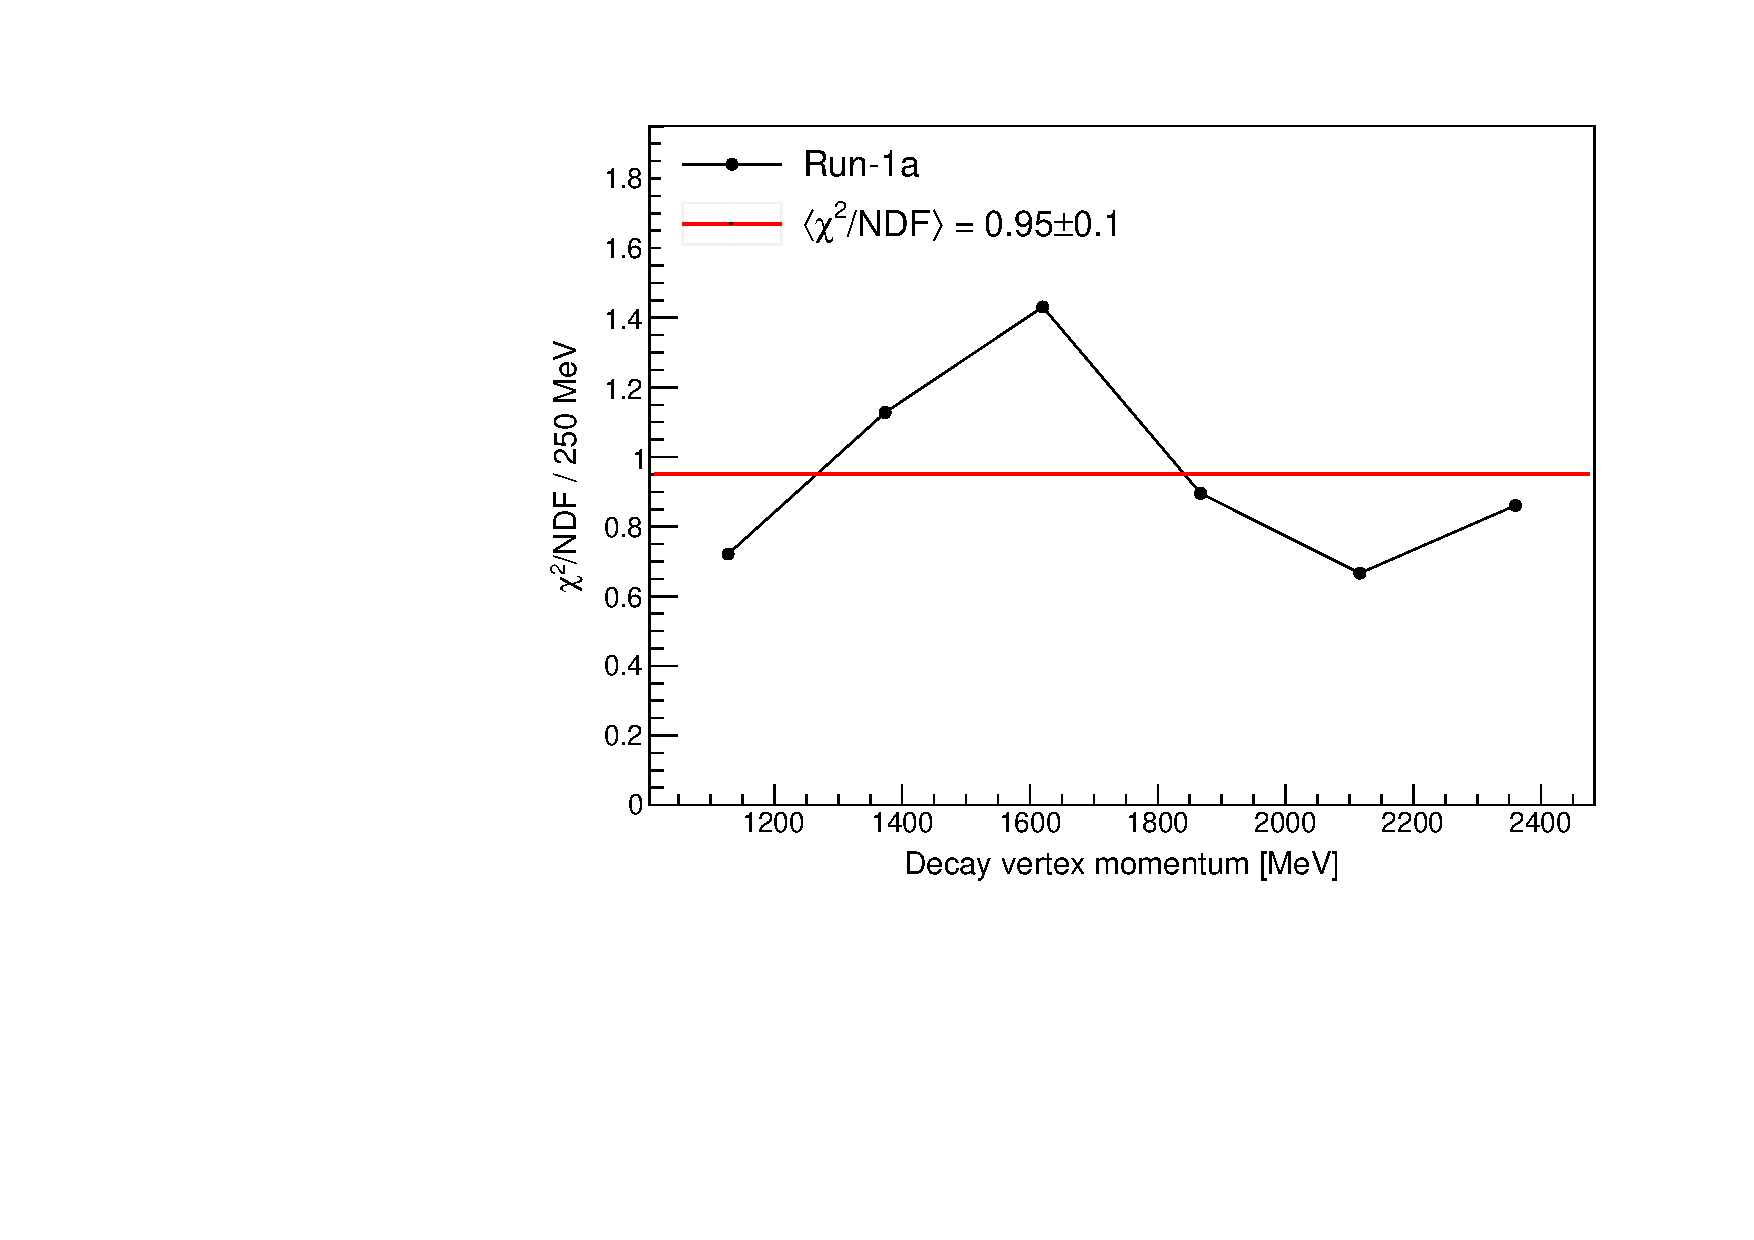
\includegraphics[trim={0 0 0 0},clip,width=.47\textwidth]{Images/Chapter6/S12S18_chi2NDF_vs_p_fit_Run-1a_250MeV_1000_2500MeV_randomised_BQ.pdf}}
\subfloat[Run-1b.]{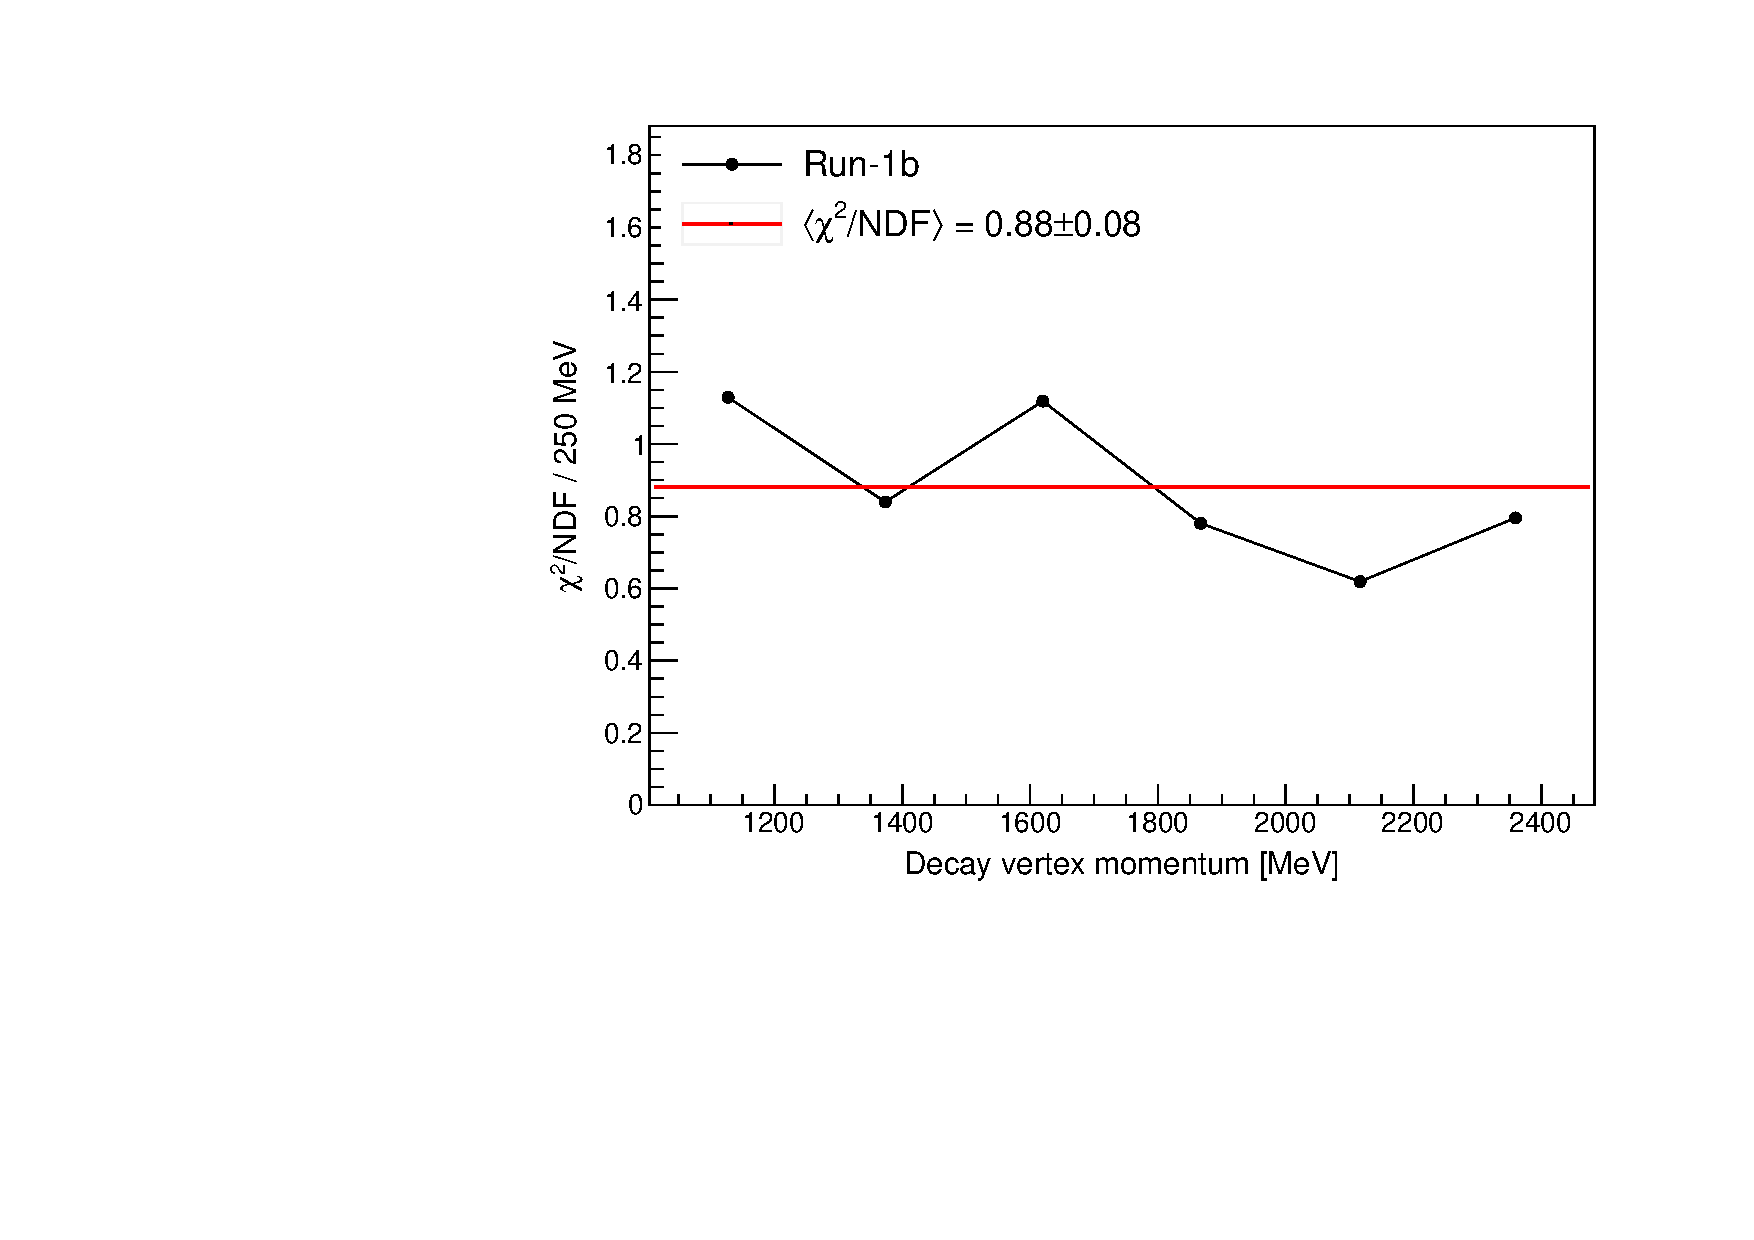
\includegraphics[trim={0 0 0 0},clip,width=.47\textwidth]{Images/Chapter6/S12S18_chi2NDF_vs_p_fit_Run-1b_250MeV_1000_2500MeV_randomised_BQ.pdf}}
\hfill
\subfloat[Run-1c.]{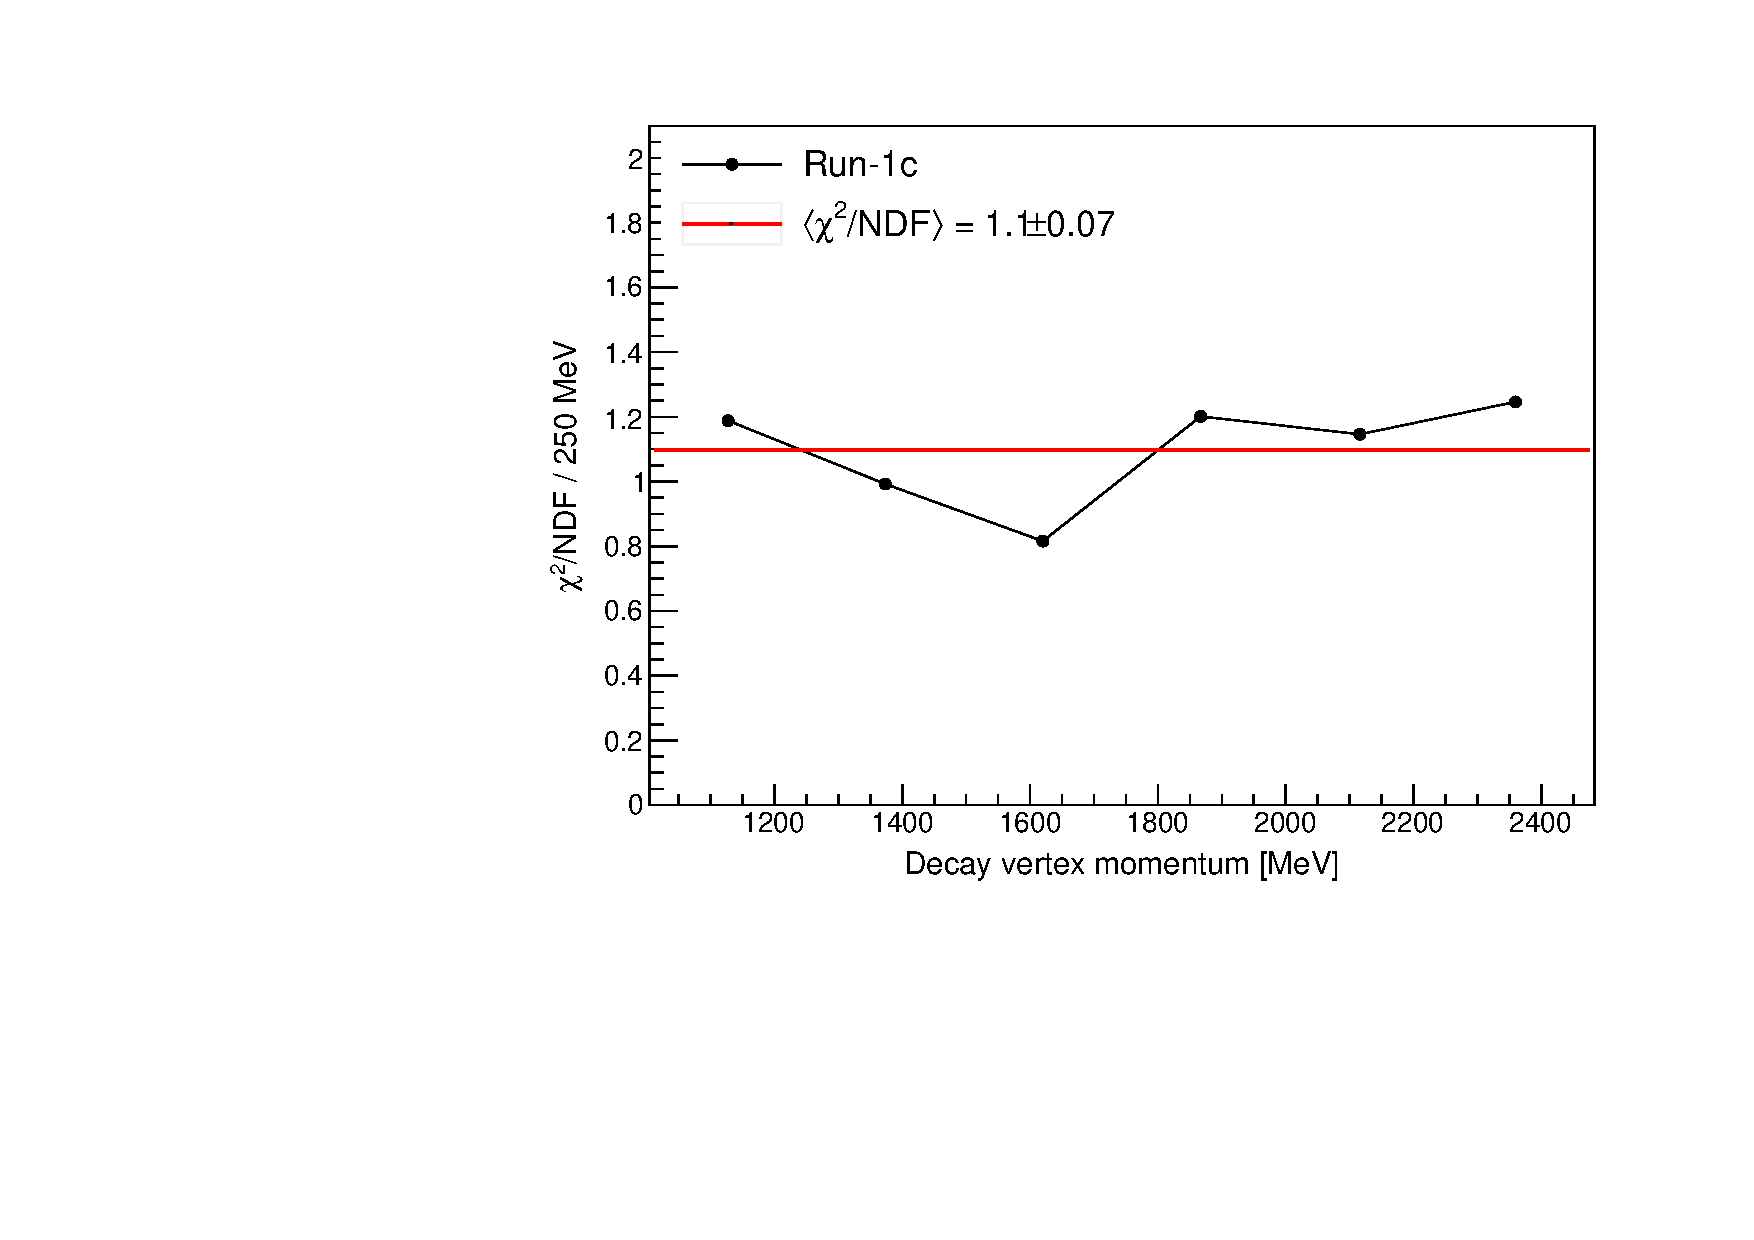
\includegraphics[trim={0 0 0 0},clip,width=.47\textwidth]{Images/Chapter6/S12S18_chi2NDF_vs_p_fit_Run-1c_250MeV_1000_2500MeV_randomised_BQ.pdf}}
\subfloat[Run-1d.]{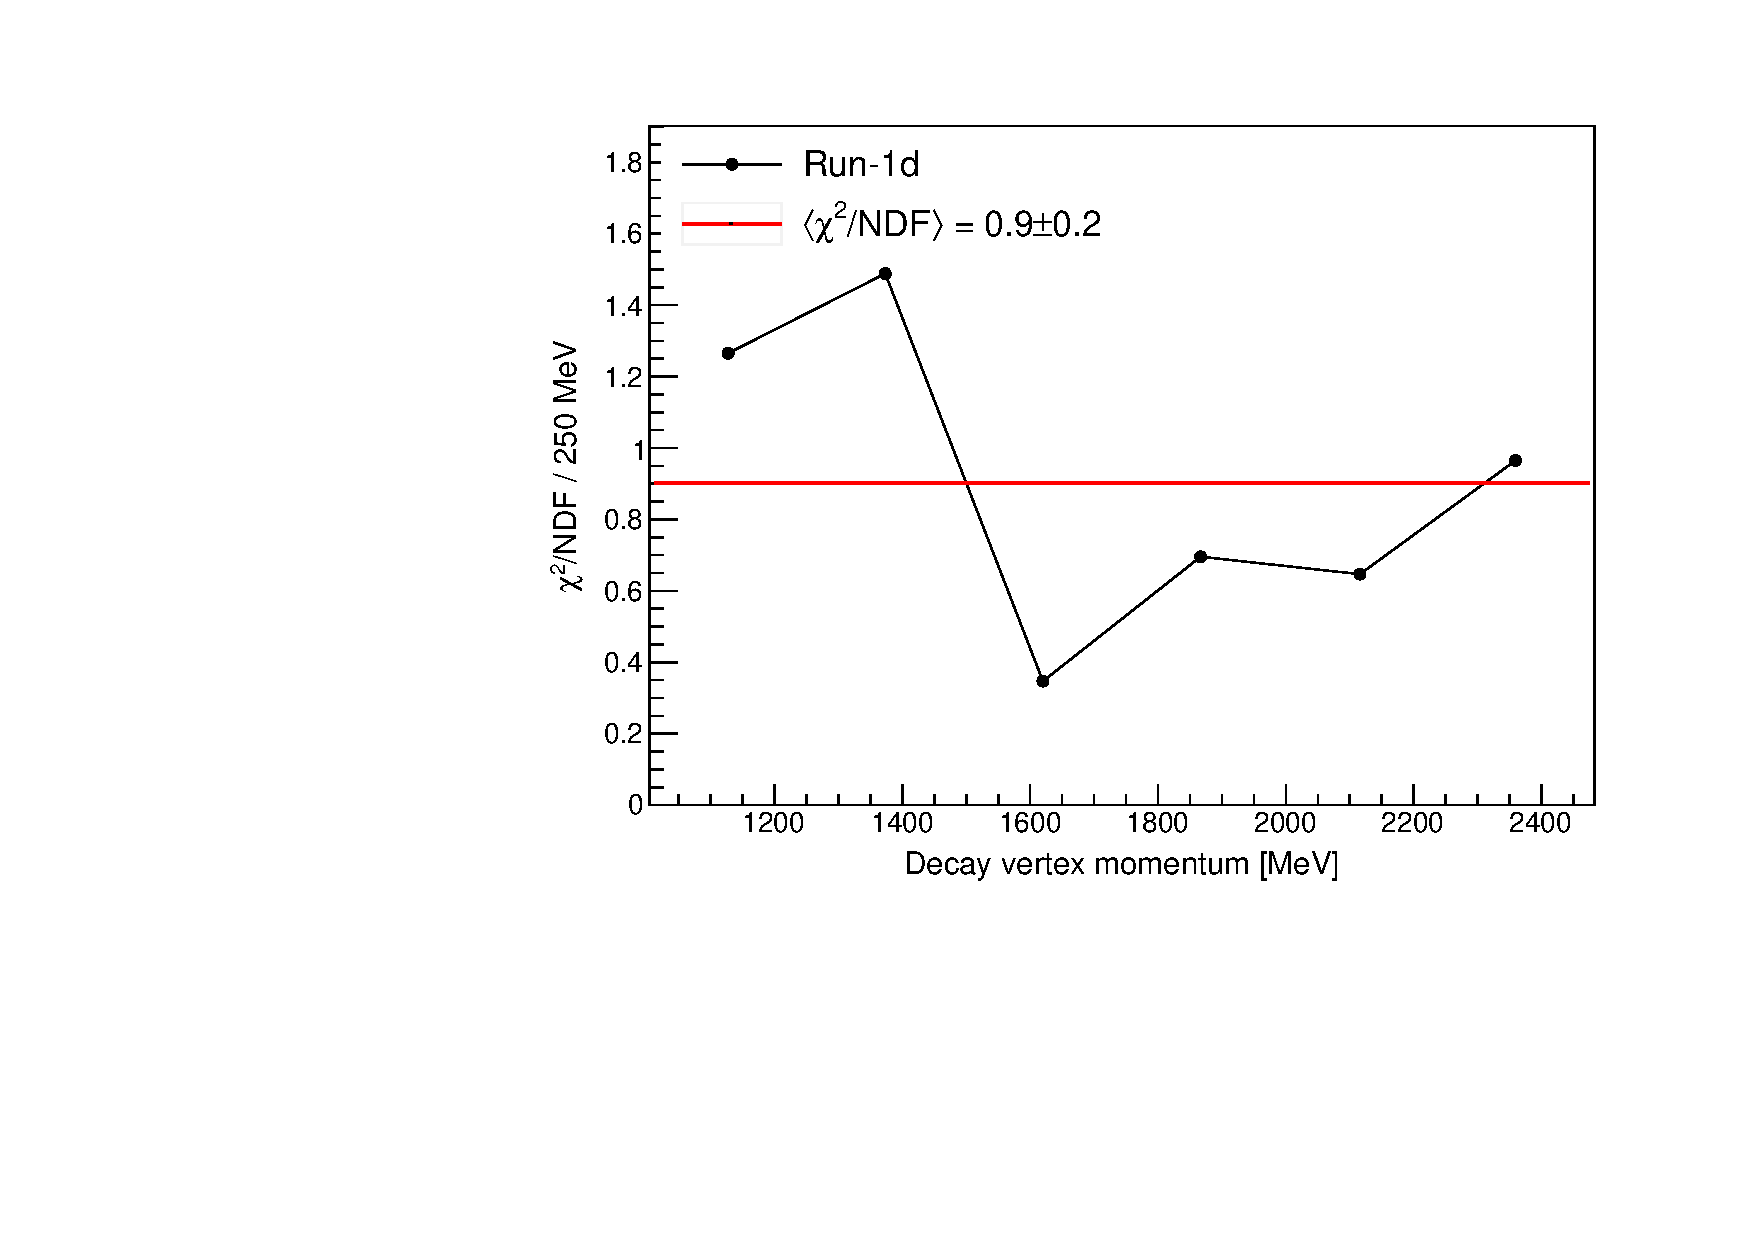
\includegraphics[trim={0 0 0 0},clip,width=.47\textwidth]{Images/Chapter6/S12S18_chi2NDF_vs_p_fit_Run-1d_250MeV_1000_2500MeV_50usStartTime_randomised_BQ.pdf}}
\caption{Fit $\chi^{2}/\text{NDF}$ per momentum bin for each Run-1 dataset, where a zeroth order polynomial fits gives the average in each case. These average values are consistent with one to within a maximum deviation of $1.5\sigma$.}
\label{fig:Chi2Run1MomBinnedFits}
\end{figure} 

% \myworries{These distributions are not necessarily expected to be consistent between bins of the same dataset, since the blind signal is weighted according to the level of dilution in that bin, however, they are expected to be consistent for different datasets in the same bin. While this can be seen to be true for the majority of bins by simple inspection of Figure \ref{fig:Run1AEDM}, the maximum standard deviation between all combinations $A_{\text{EDM}}^{\text{BLIND}}$ values measured using different datasets, per momentum bin, is expressed by in Figure \ref{fig:Run1AEDMSigmaMax}. The greatest deviation is $\sim2.5\sigma$, which may be attributed to statistical fluctuations.}

% \begin{figure}[h!]
% \centering{}
% 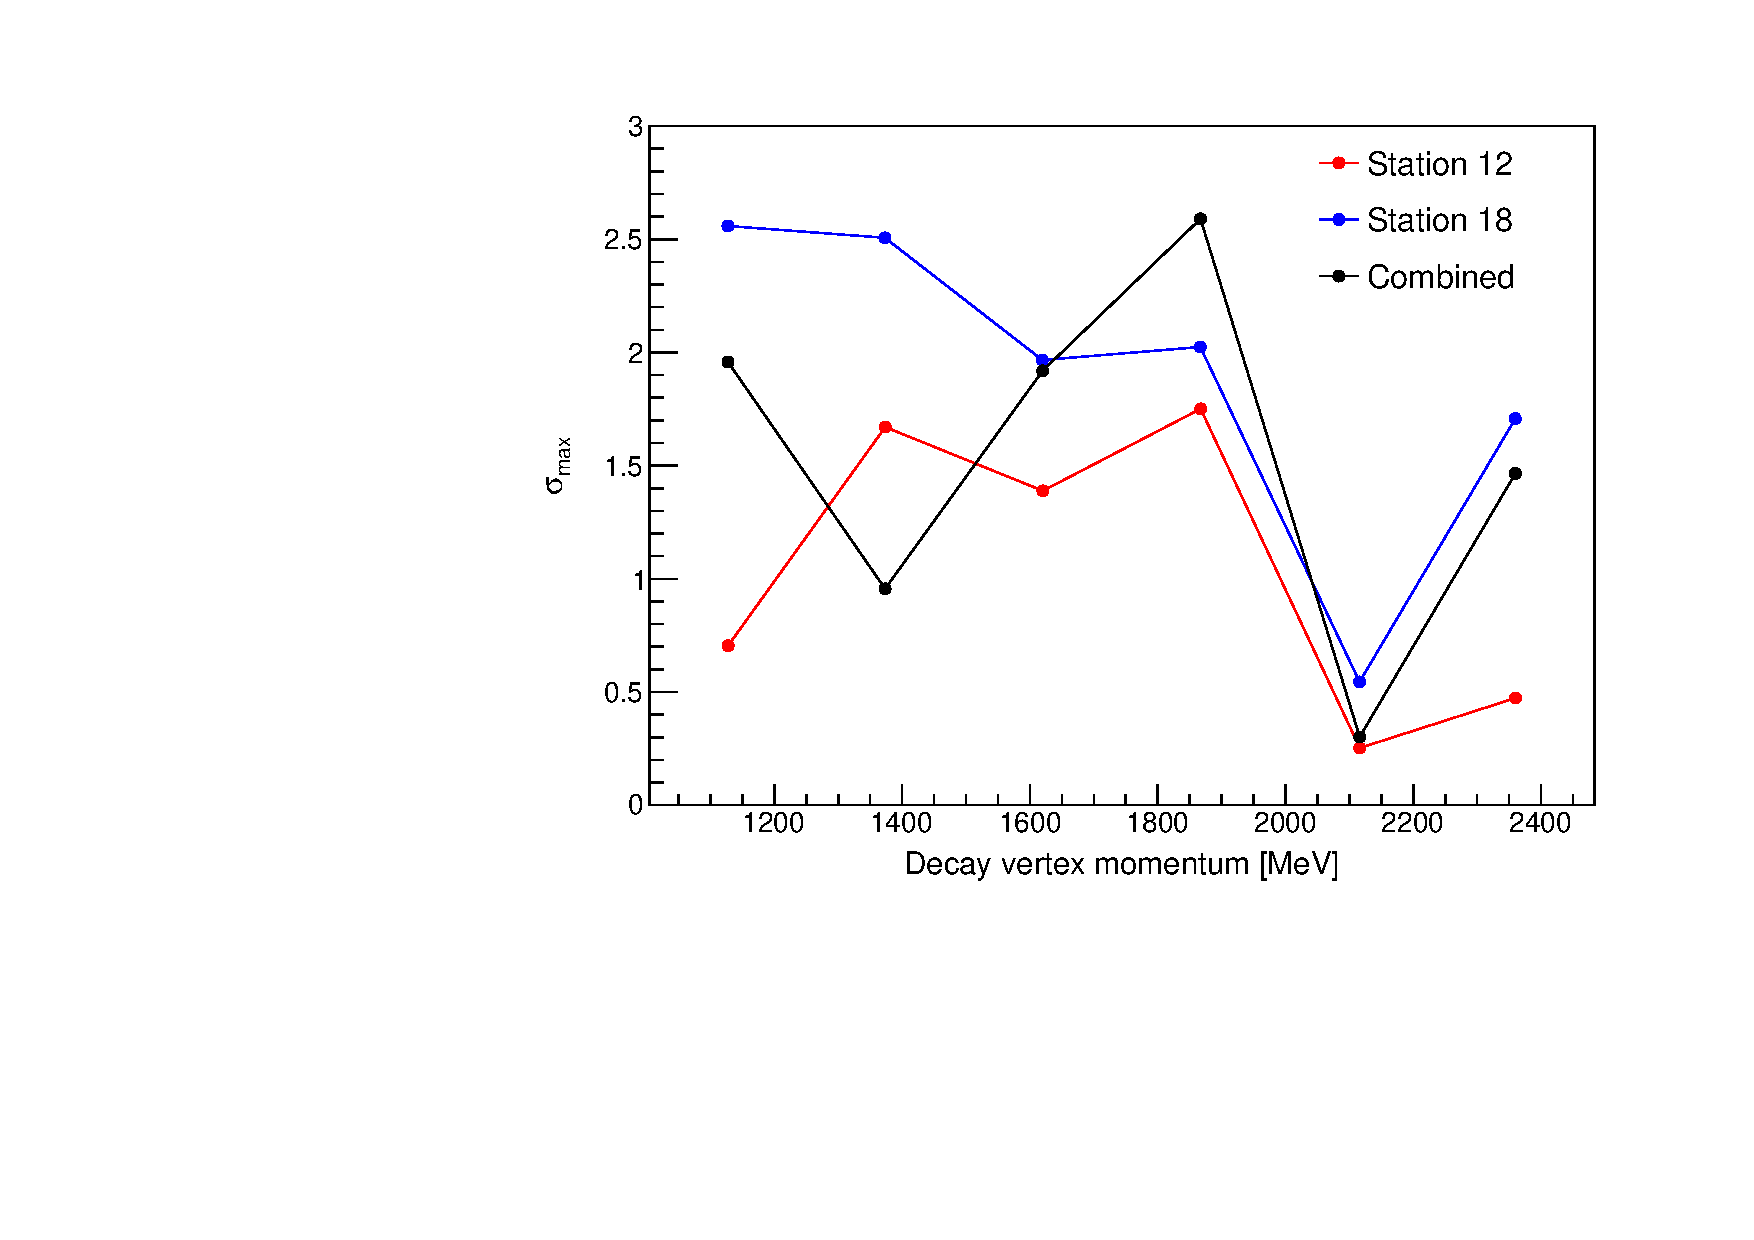
\includegraphics[trim={0 0 0 0},clip,width=.49\textwidth]{Images/Chapter6/AEDM_max_sigma_vs_p_overlay_1000_2500.pdf}
% \caption{The maximum number of standard deviations separating $A_{\text{EDM}}^{\text{BLIND}}$ values measured in different datasets, per momentum bin. \myworries{Not so sure about this plot.}}
% \label{fig:Run1AEDMSigmaMax}
% \end{figure} 

\clearpage

\begin{figure}[]
\centering{}
\subfloat[1000-1250 MeV.]{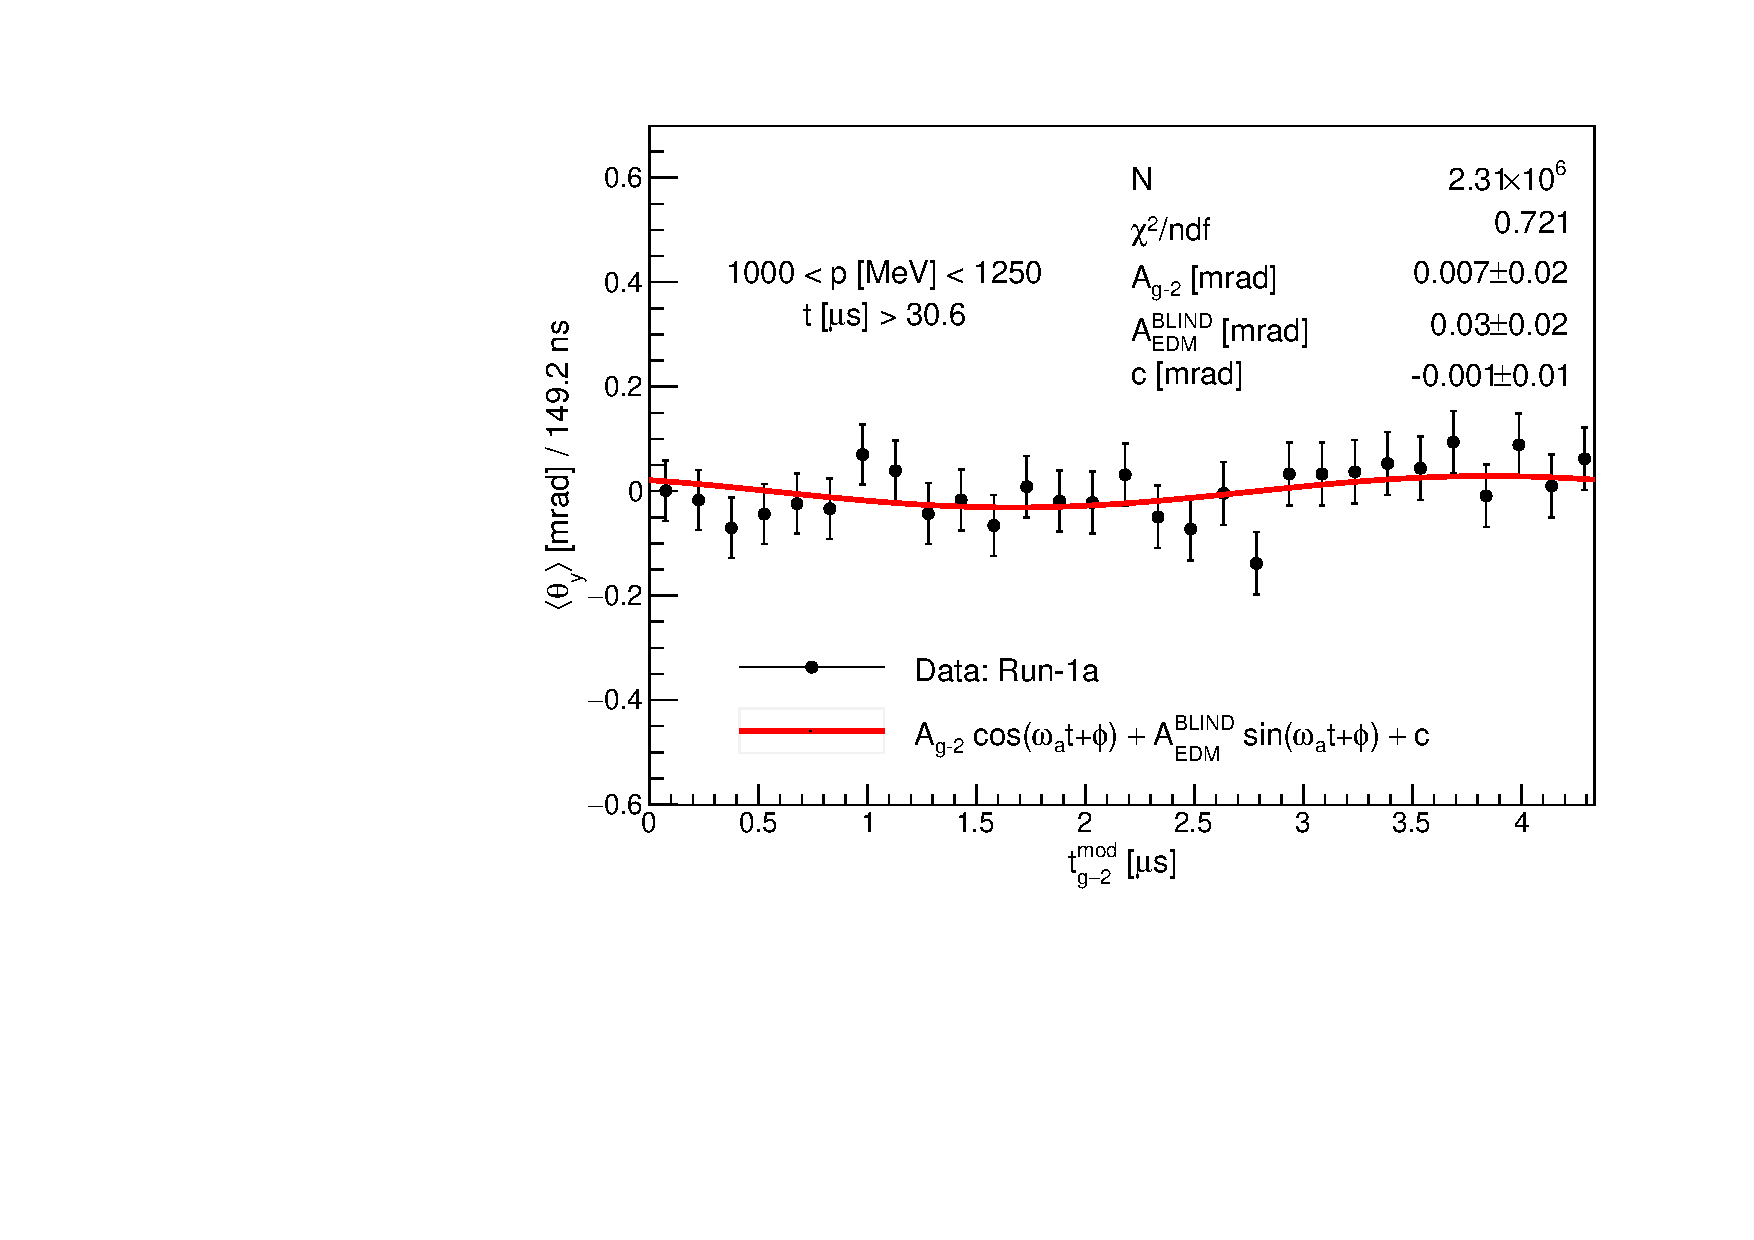
\includegraphics[trim={0 0 0 0},clip,width=.49\textwidth]{Images/Chapter6/S12S18_edmFit_1000_1250_Run-1a_250MeV_BQ.pdf}}
\subfloat[1250-1500 MeV.]{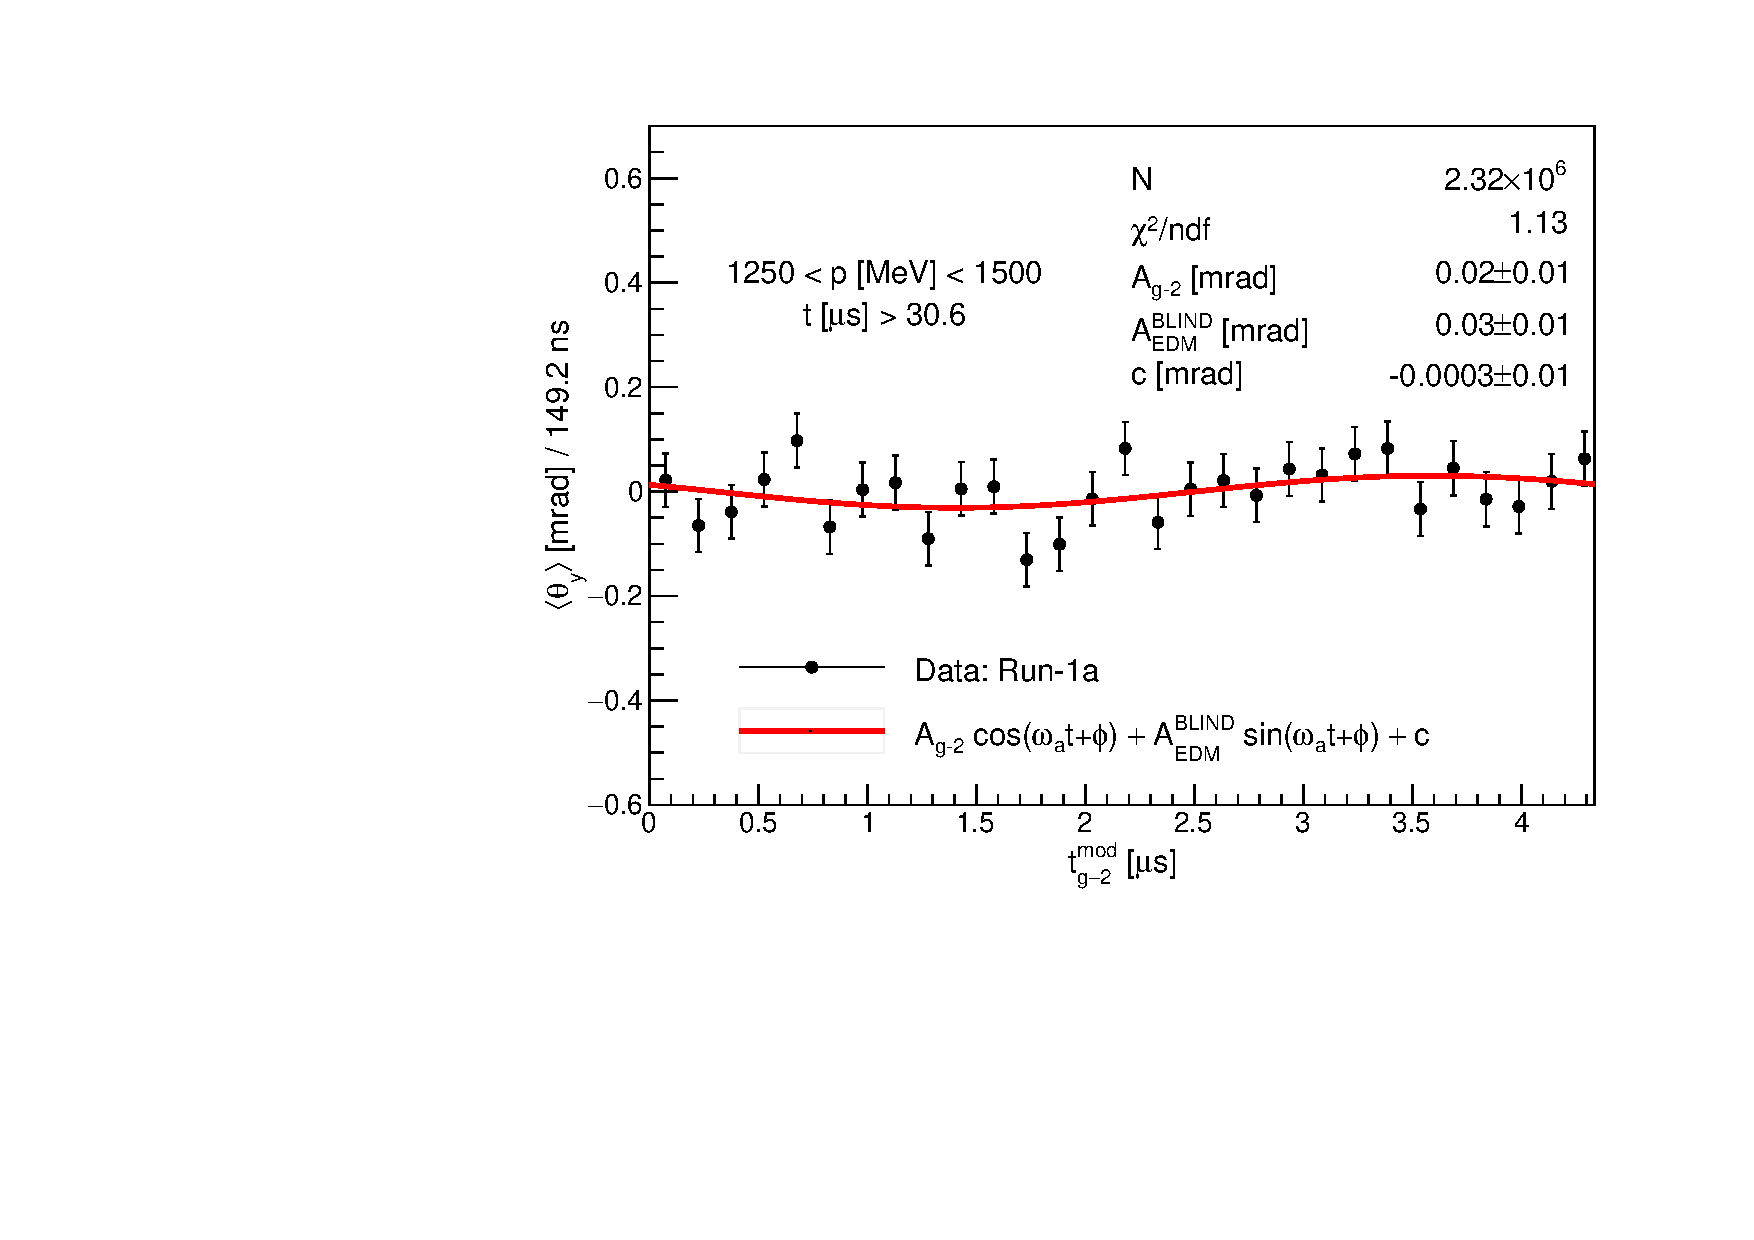
\includegraphics[trim={0 0 0 0},clip,width=.49\textwidth]{Images/Chapter6/S12S18_edmFit_1250_1500_Run-1a_250MeV_BQ.pdf}}
\hfill
\subfloat[1500-1750 MeV.]{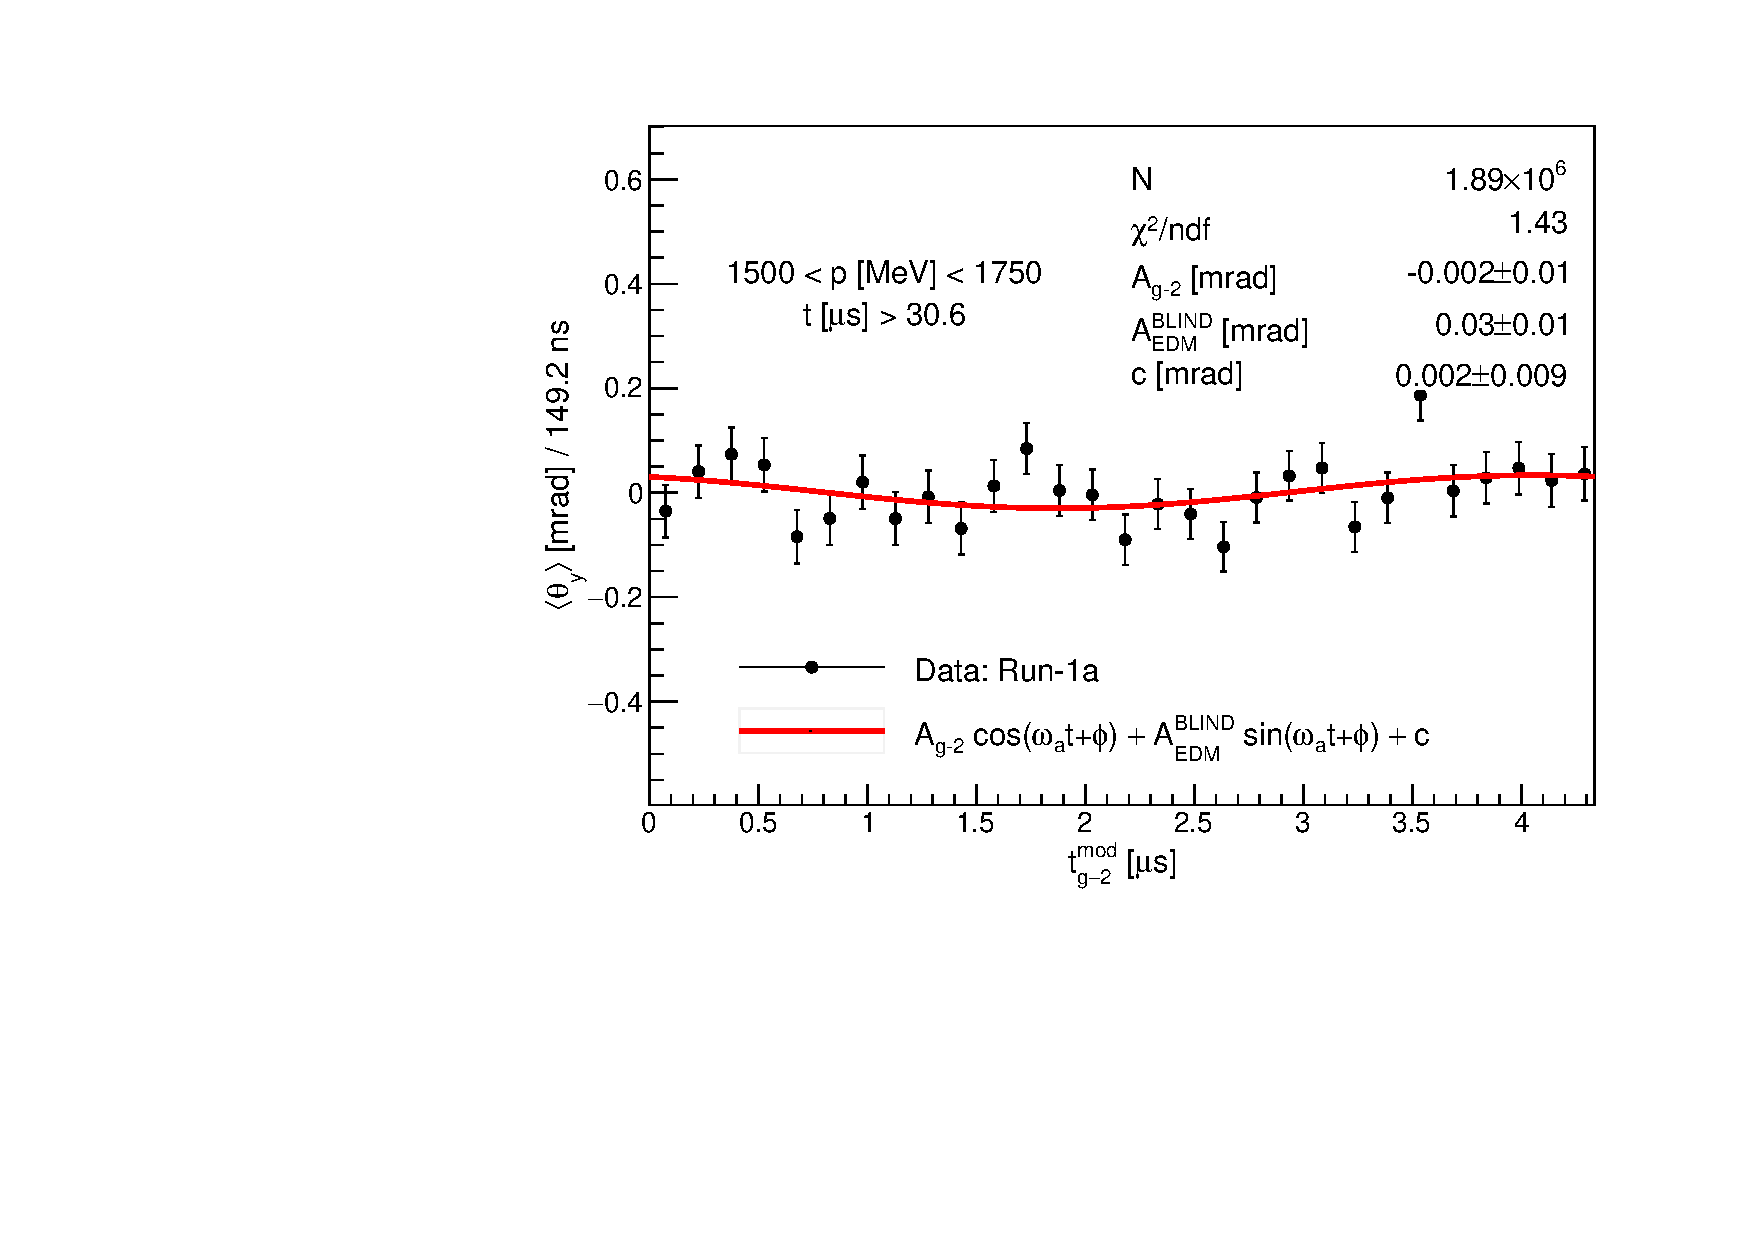
\includegraphics[trim={0 0 0 0},clip,width=.49\textwidth]{Images/Chapter6/S12S18_edmFit_1500_1750_Run-1a_250MeV_BQ.pdf}}
\subfloat[1750-2000 MeV.]{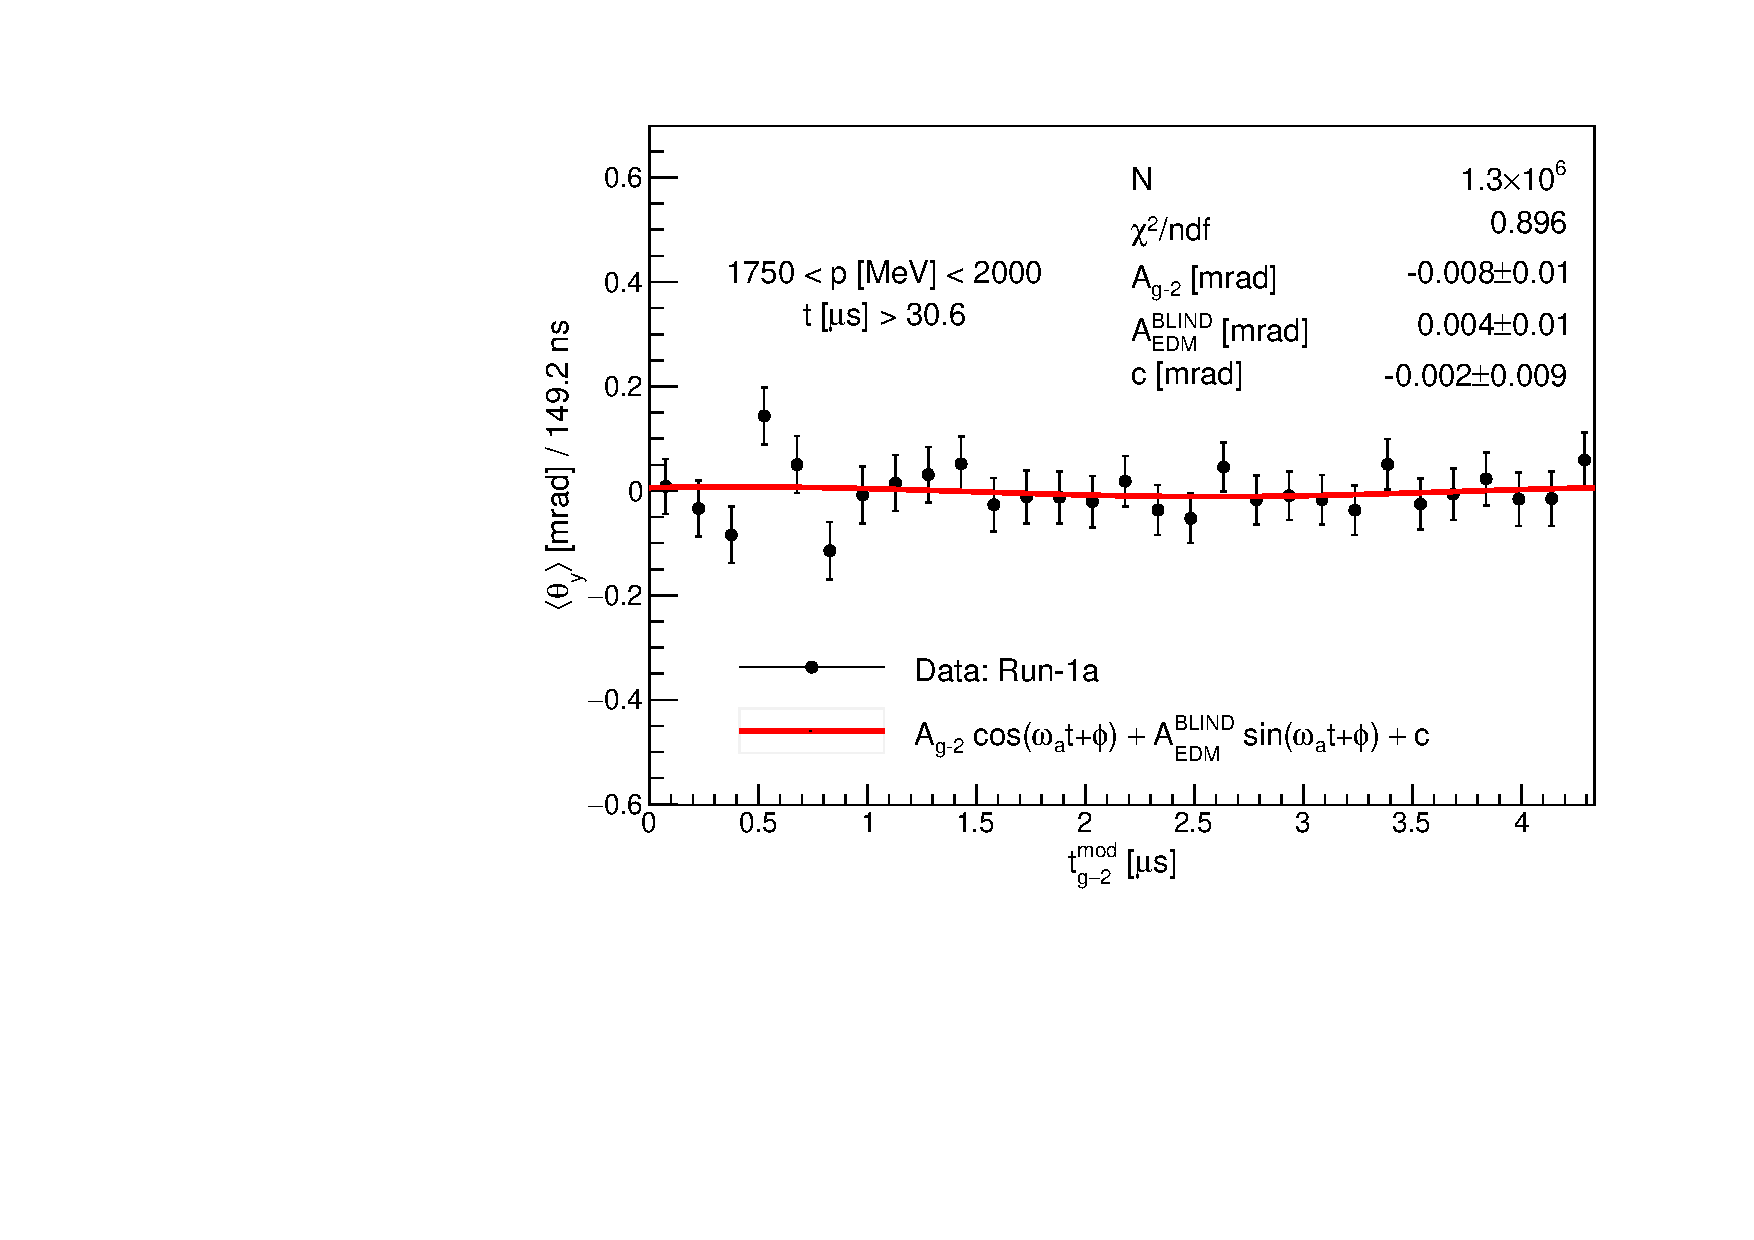
\includegraphics[trim={0 0 0 0},clip,width=.49\textwidth]{Images/Chapter6/S12S18_edmFit_1750_2000_Run-1a_250MeV_BQ.pdf}}
\hfill
\subfloat[2000-2250 MeV.]{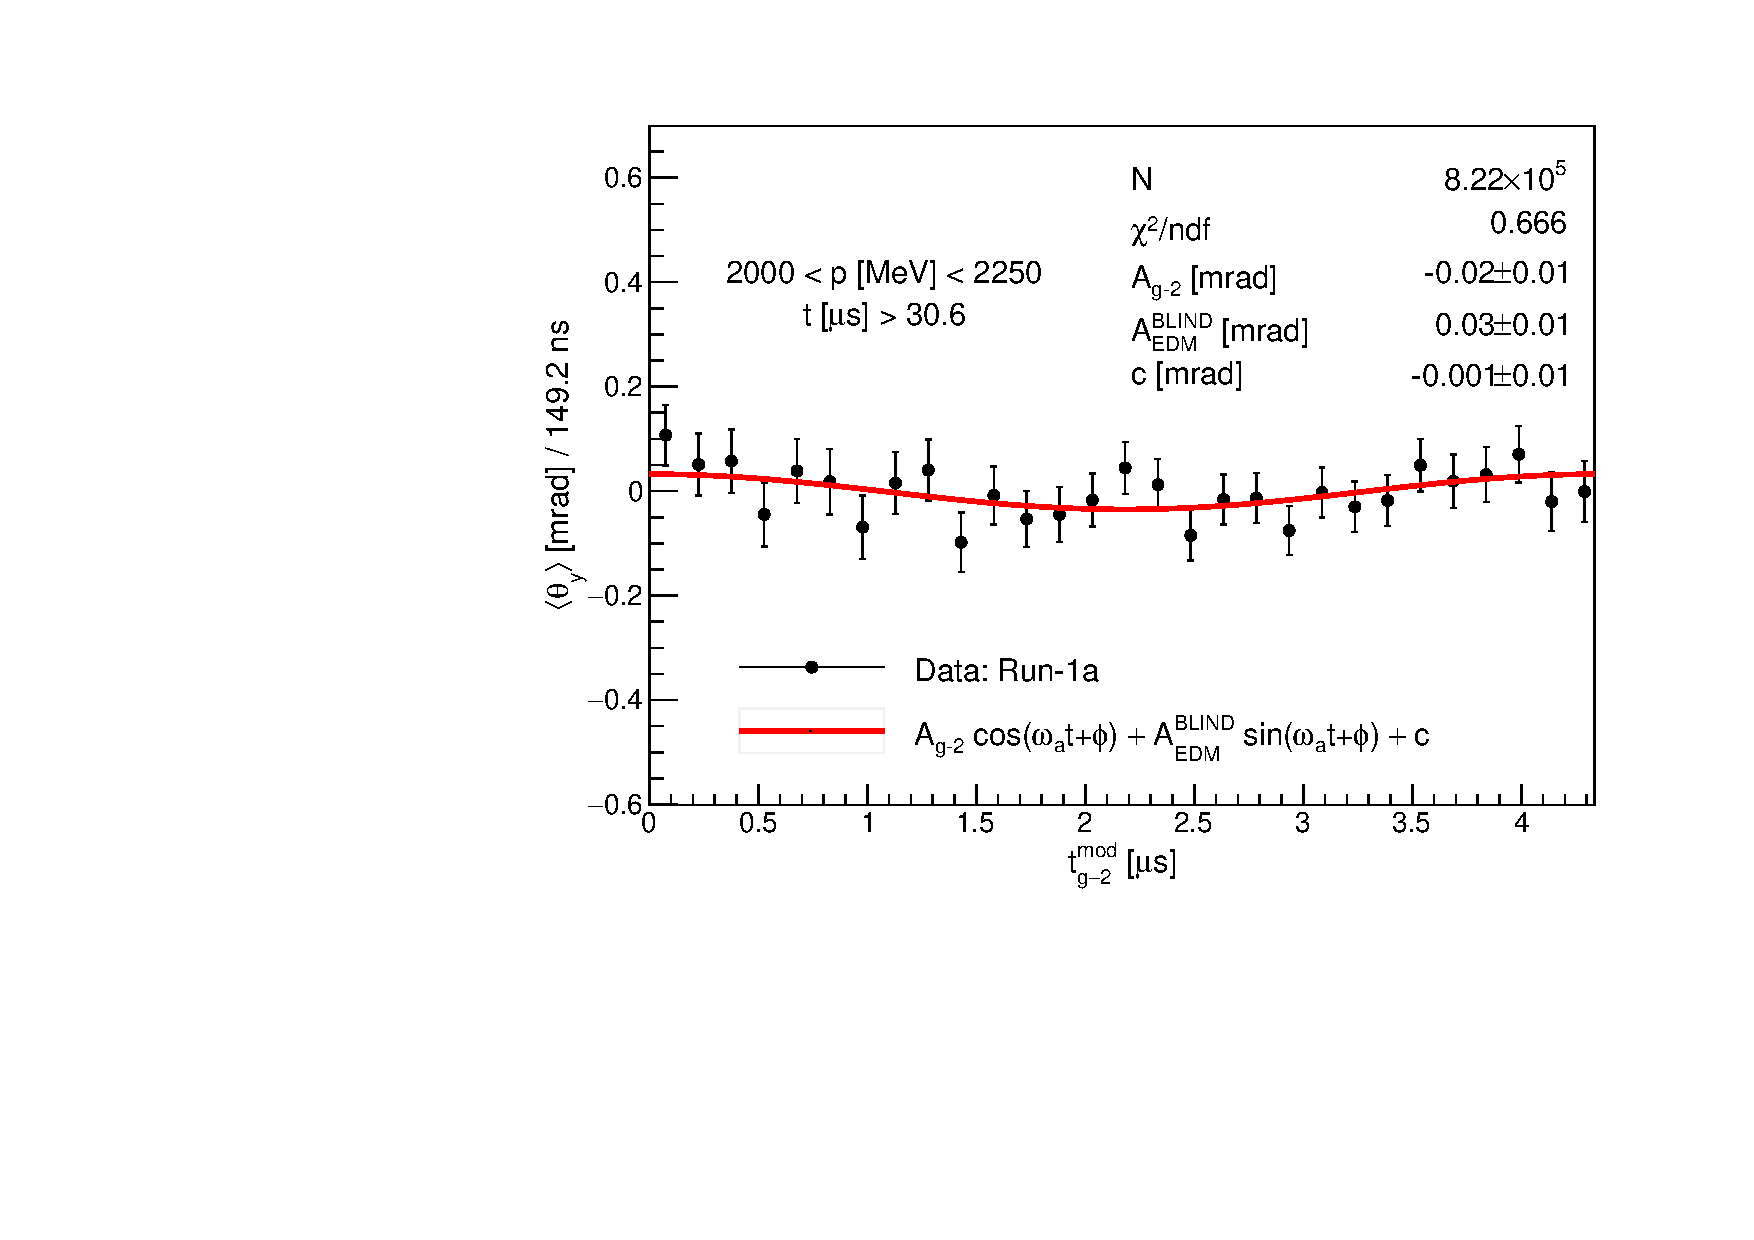
\includegraphics[trim={0 0 0 0},clip,width=.49\textwidth]{Images/Chapter6/S12S18_edmFit_2000_2250_Run-1a_250MeV_BQ.pdf}}
\subfloat[2250-2500 MeV.]{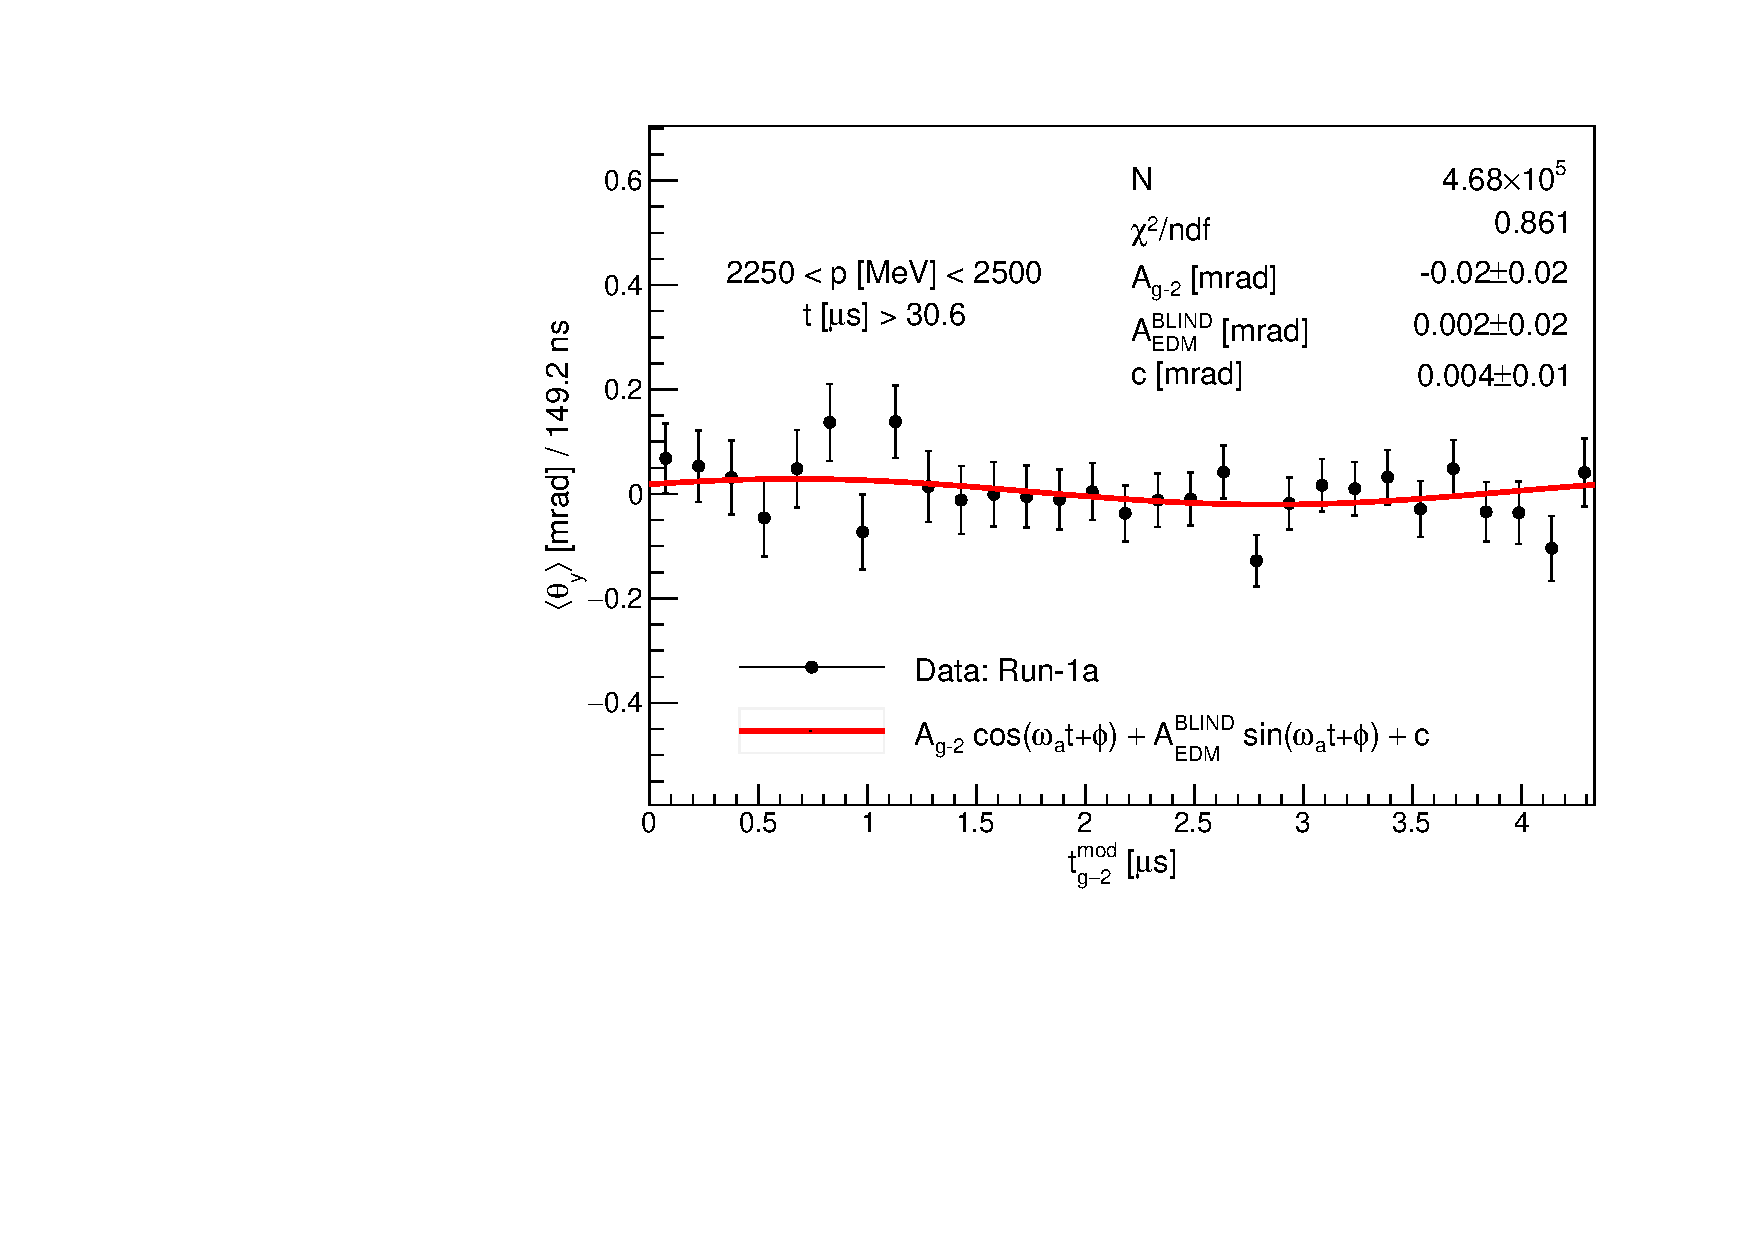
\includegraphics[trim={0 0 0 0},clip,width=.49\textwidth]{Images/Chapter6/S12S18_edmFit_2250_2500_Run-1a_250MeV_BQ.pdf}}
\caption{Momentum-binned vertical angle oscillation fits for Run-1a. Tracker stations 12 and 18 are combined.}
\label{fig:Run1aMomBinnedFits}
\end{figure} 
\clearpage

\begin{figure}[]
\centering{}
\subfloat[1000-1250 MeV.]{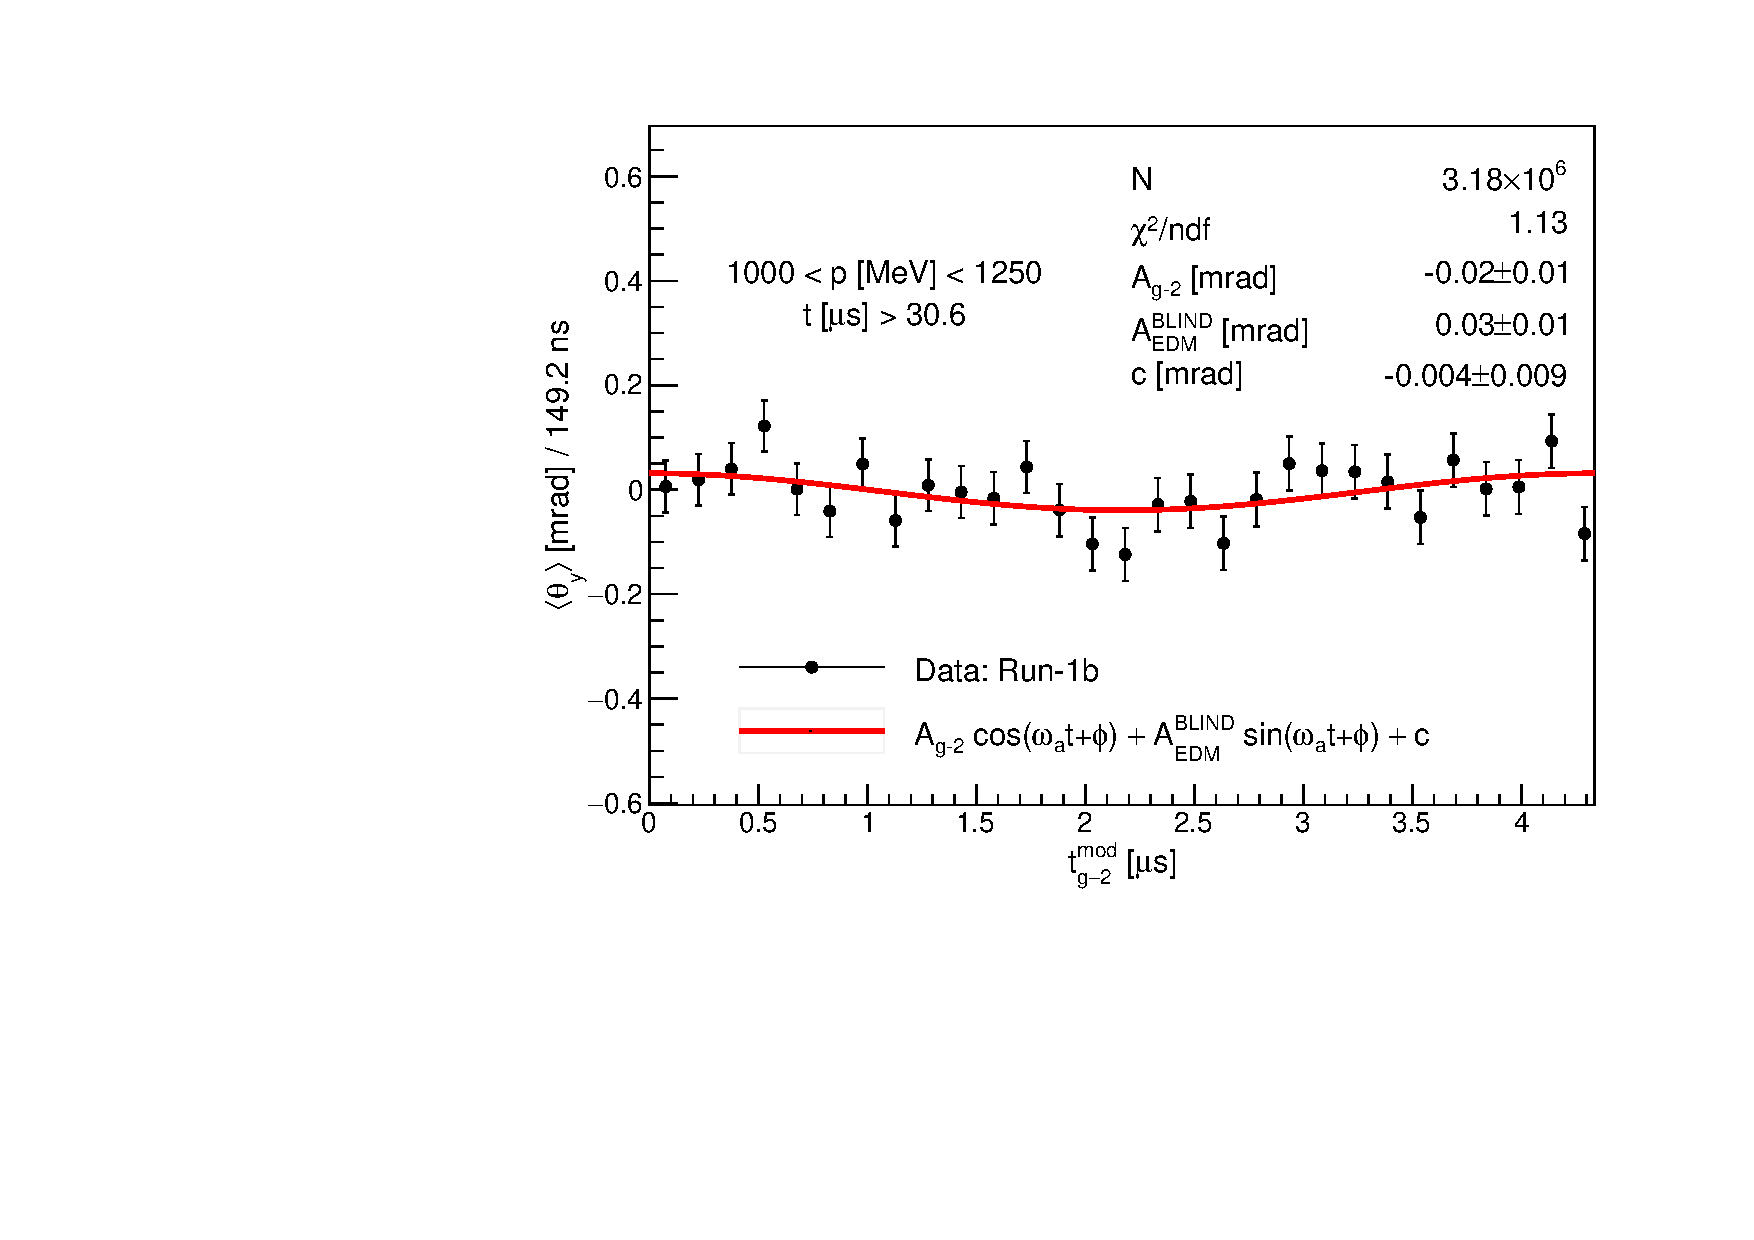
\includegraphics[trim={0 0 0 0},clip,width=.49\textwidth]{Images/Chapter6/S12S18_edmFit_1000_1250_Run-1b_250MeV_BQ.pdf}}
\subfloat[1250-1500 MeV.]{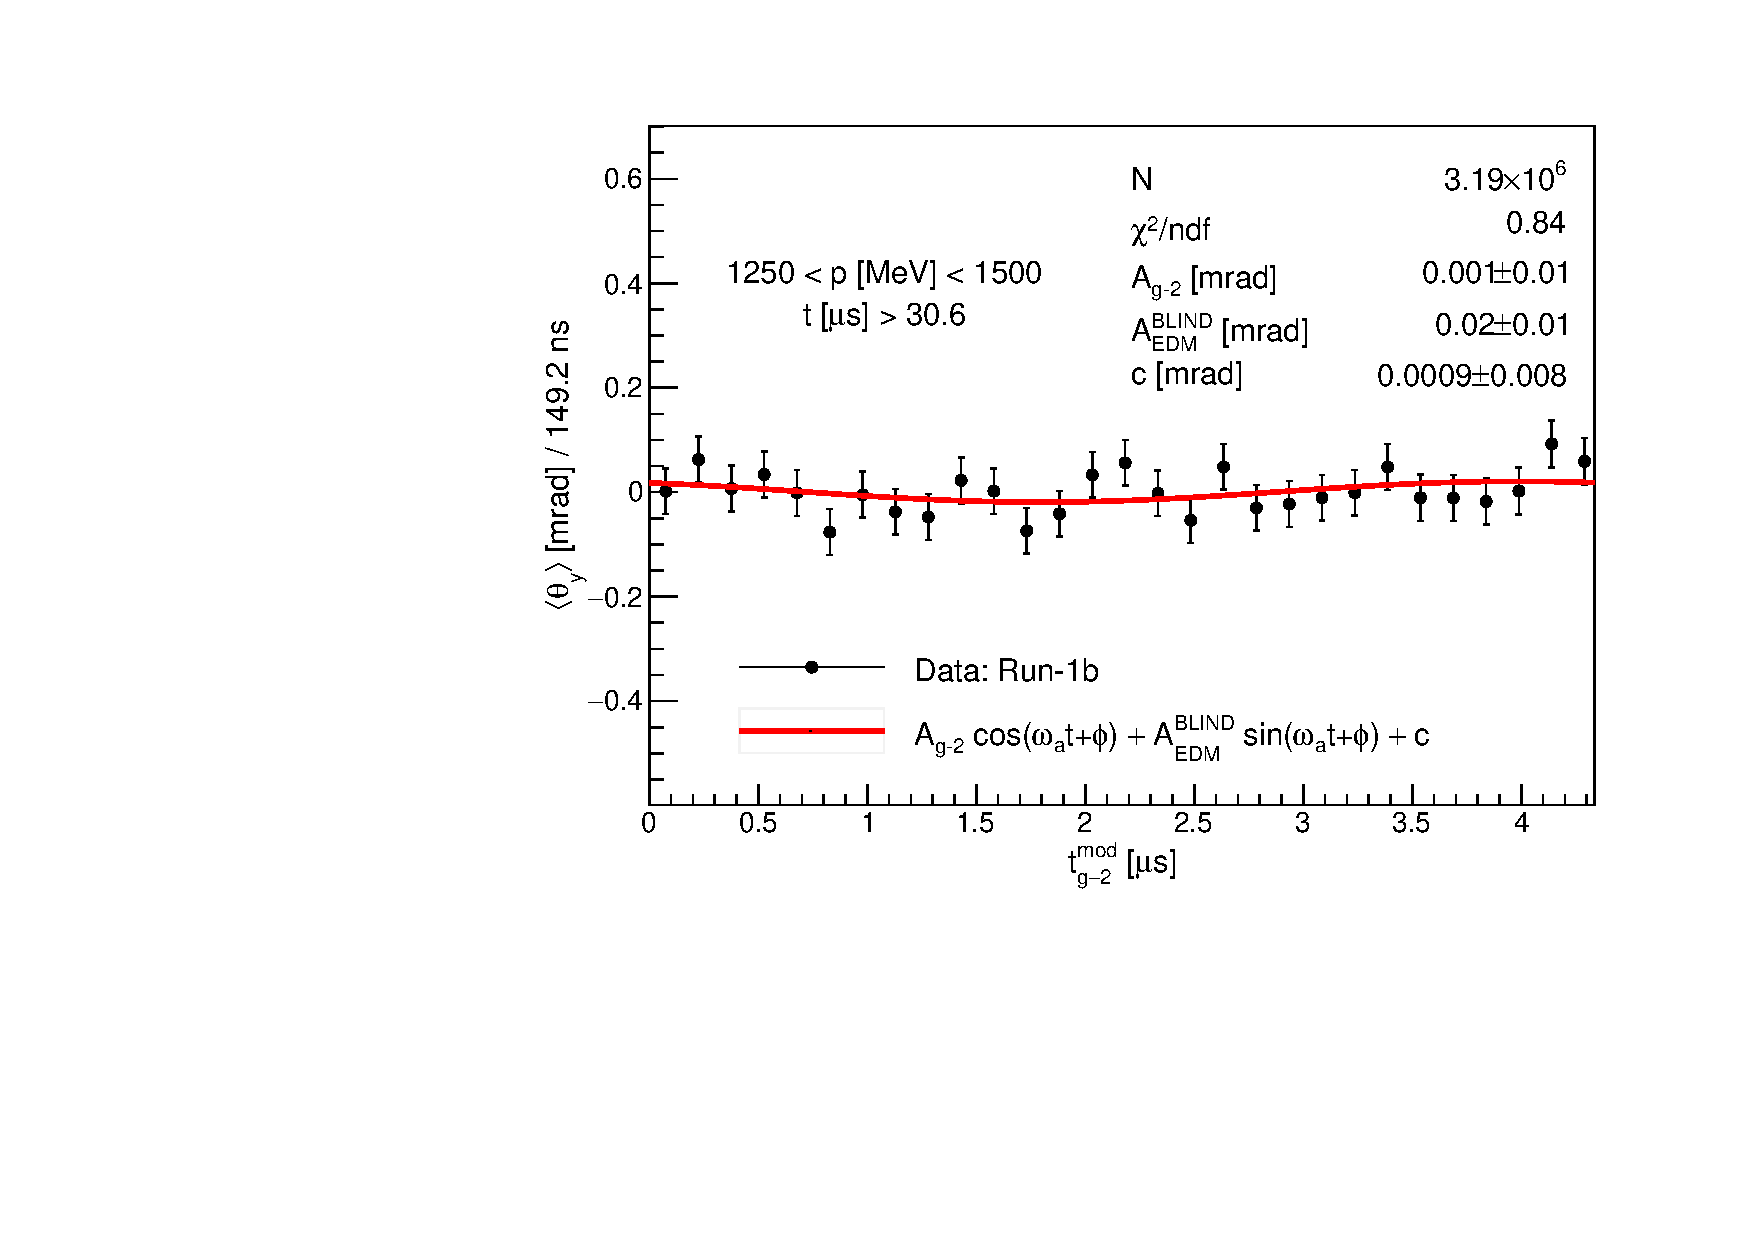
\includegraphics[trim={0 0 0 0},clip,width=.49\textwidth]{Images/Chapter6/S12S18_edmFit_1250_1500_Run-1b_250MeV_BQ.pdf}}
\hfill
\subfloat[1500-1750 MeV.]{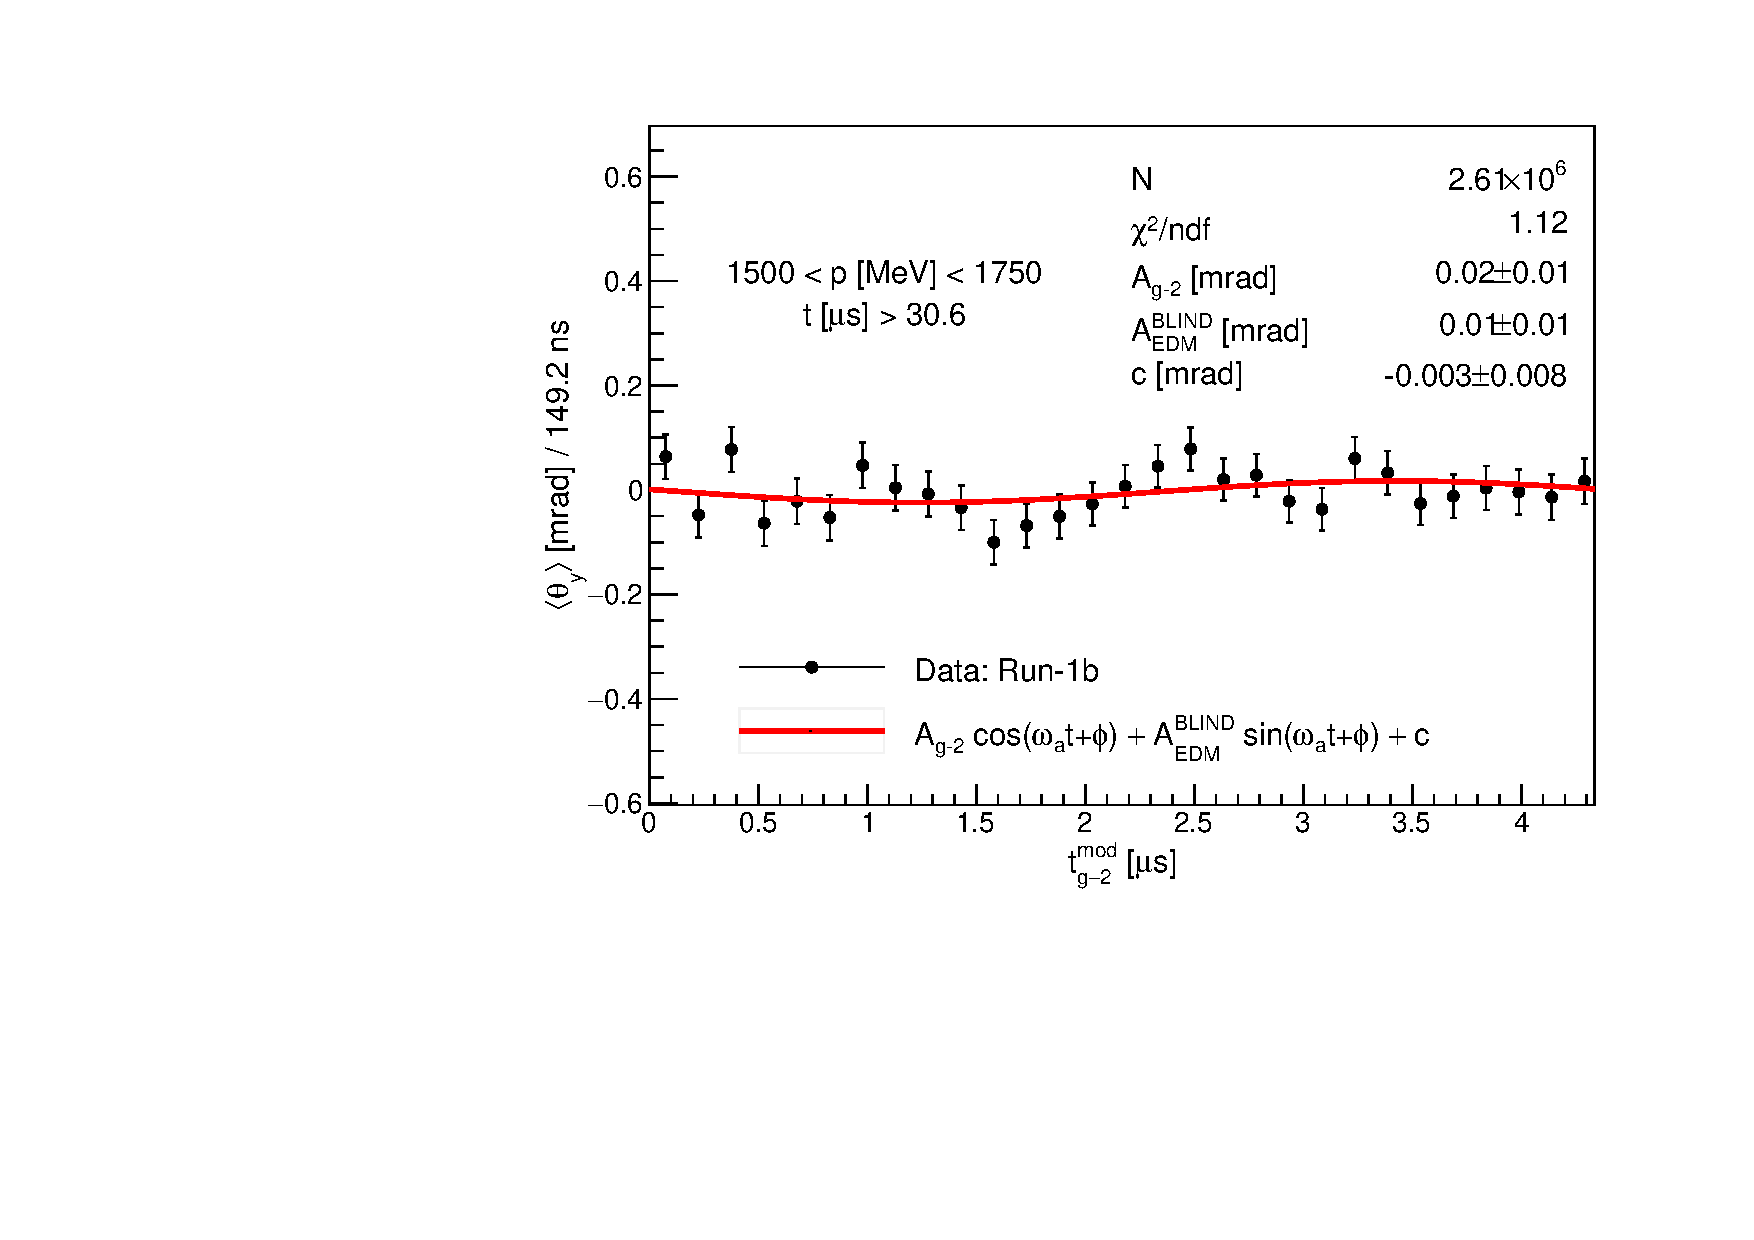
\includegraphics[trim={0 0 0 0},clip,width=.49\textwidth]{Images/Chapter6/S12S18_edmFit_1500_1750_Run-1b_250MeV_BQ.pdf}}
\subfloat[1750-2000 MeV.]{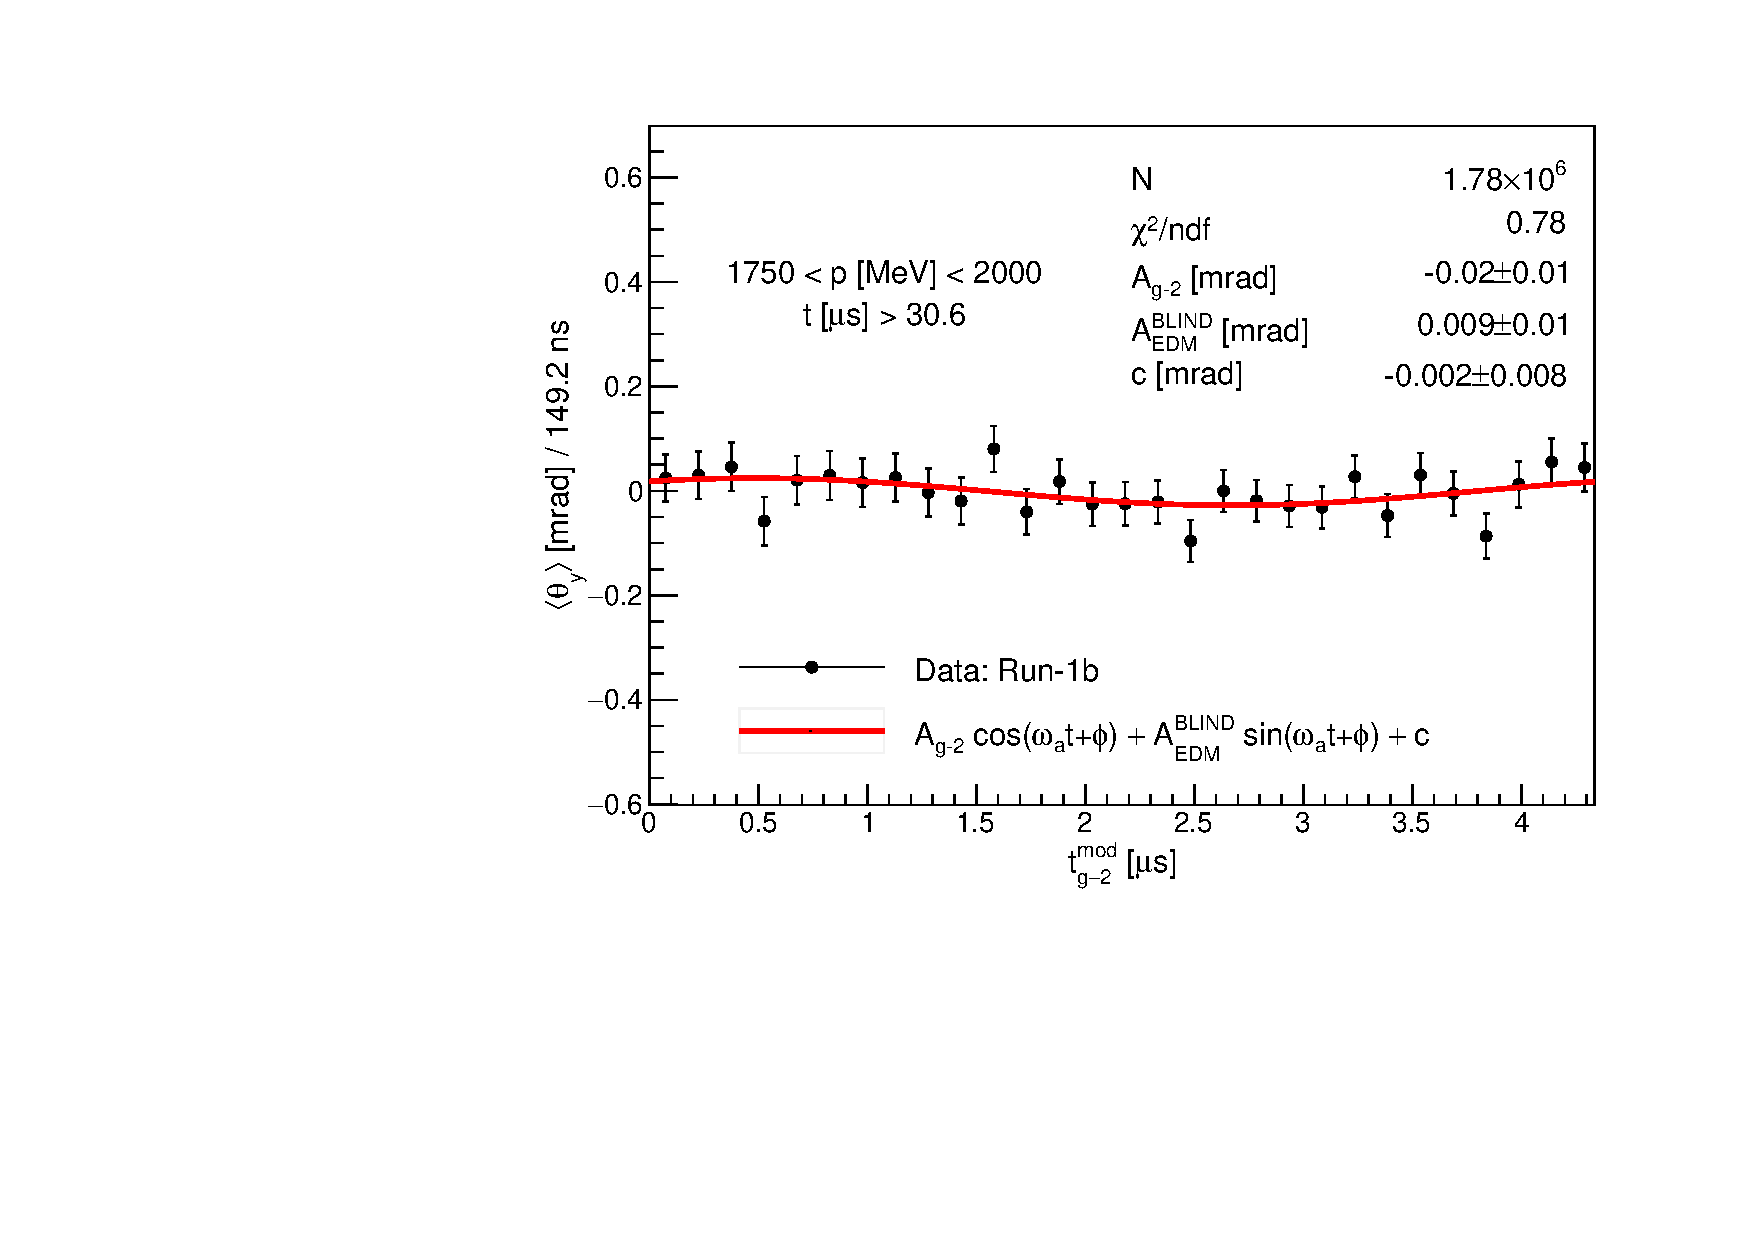
\includegraphics[trim={0 0 0 0},clip,width=.49\textwidth]{Images/Chapter6/S12S18_edmFit_1750_2000_Run-1b_250MeV_BQ.pdf}}
\hfill
\subfloat[2000-2250 MeV.]{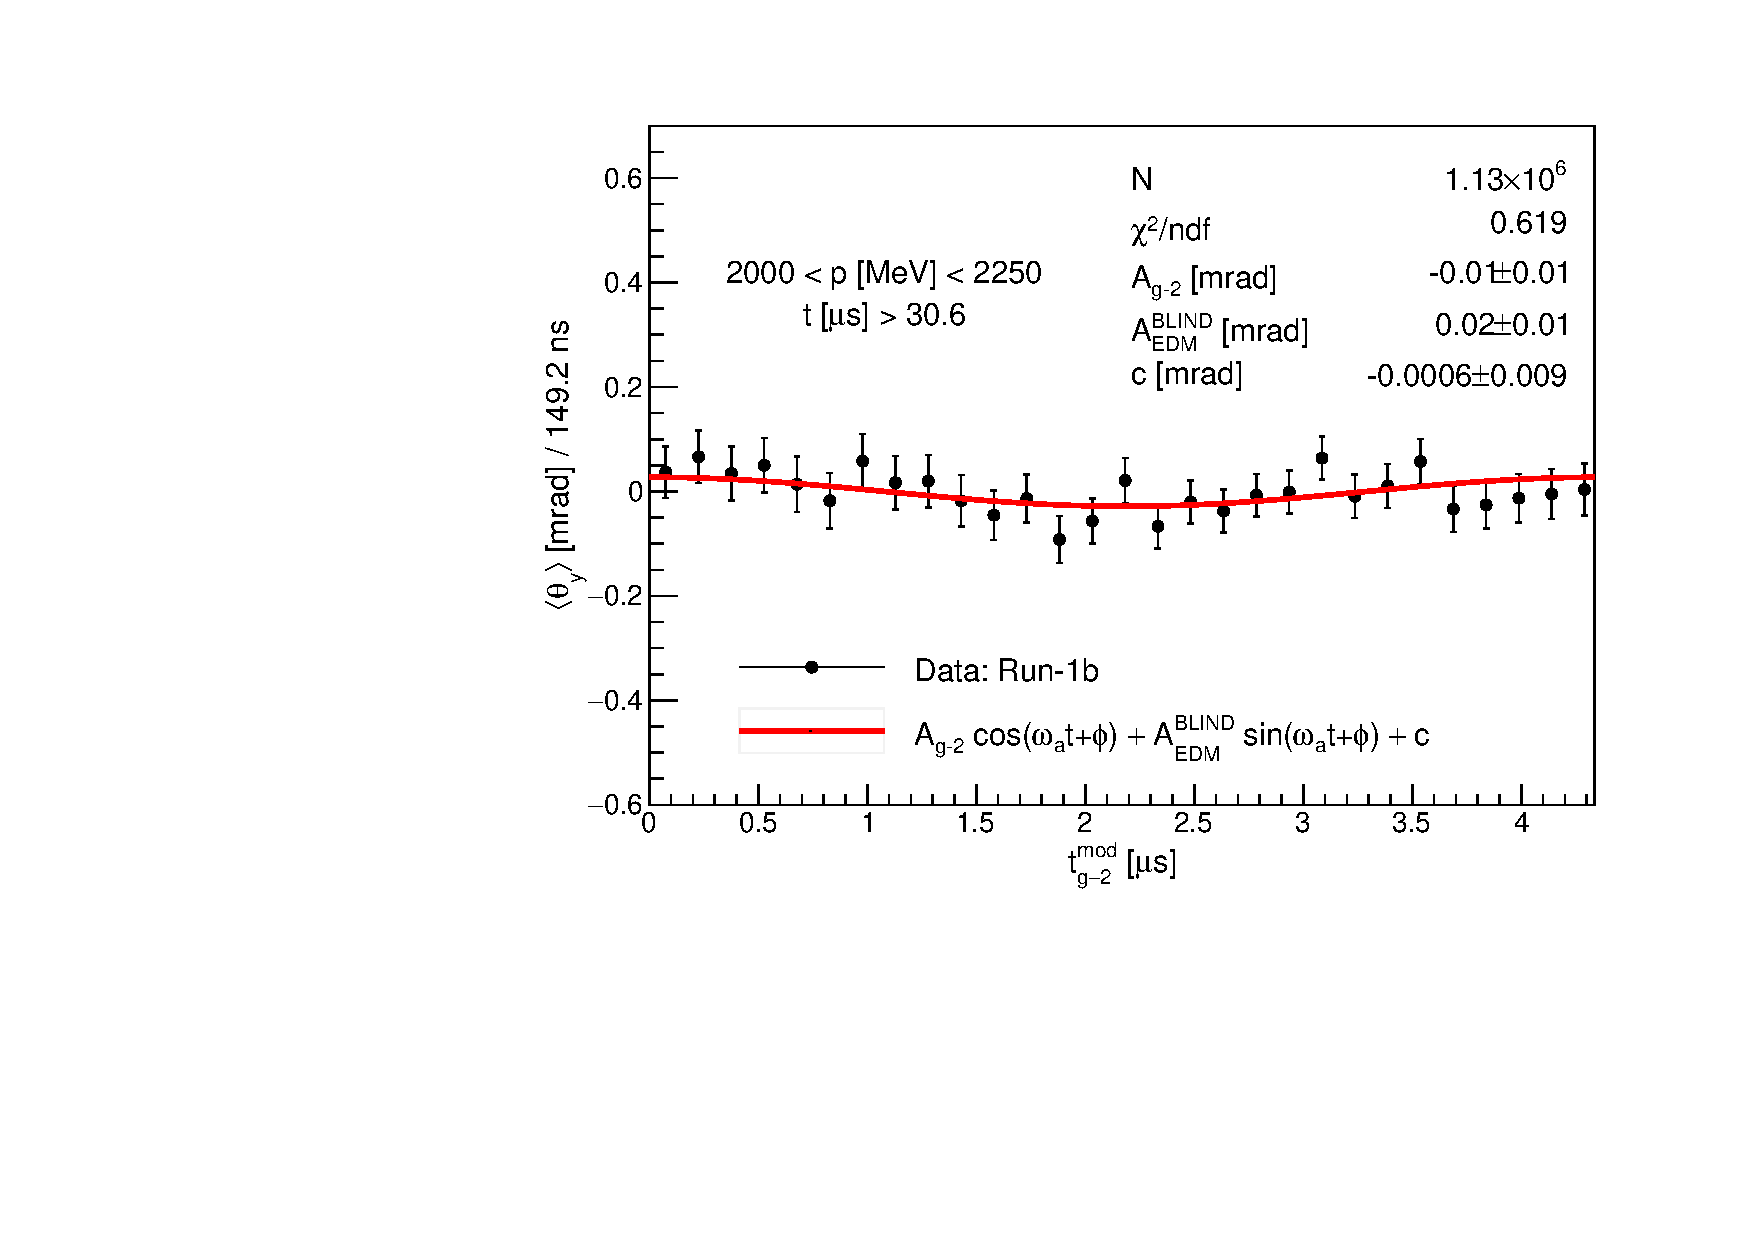
\includegraphics[trim={0 0 0 0},clip,width=.49\textwidth]{Images/Chapter6/S12S18_edmFit_2000_2250_Run-1b_250MeV_BQ.pdf}}
\subfloat[2250-2500 MeV.]{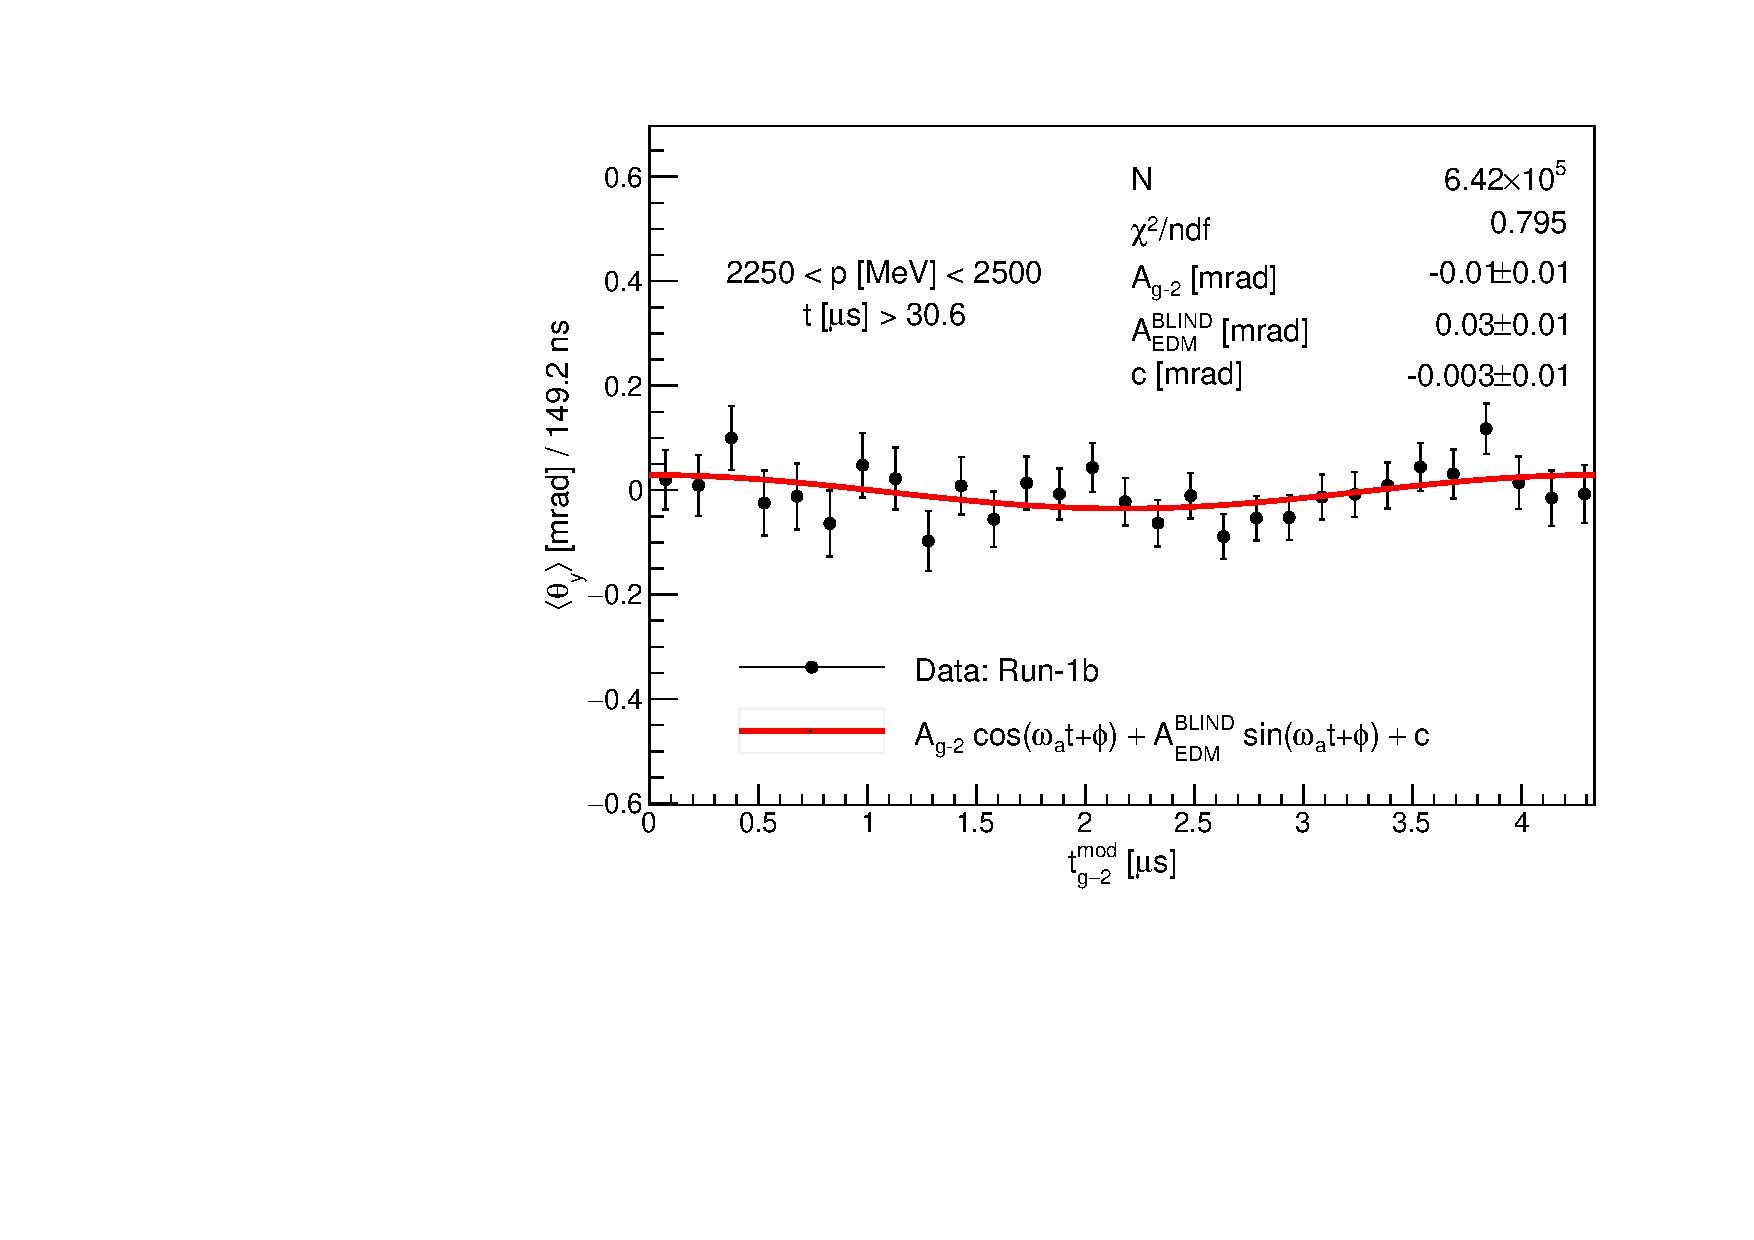
\includegraphics[trim={0 0 0 0},clip,width=.49\textwidth]{Images/Chapter6/S12S18_edmFit_2250_2500_Run-1b_250MeV_BQ.pdf}}
\caption{Momentum-binned vertical angle oscillation fits for Run-1b. Tracker stations 12 and 18 are combined.}
\label{fig:Run1bMomBinnedFits}
\end{figure} 
\clearpage

\begin{figure}[]
\centering{}
\subfloat[1000-1250 MeV.]{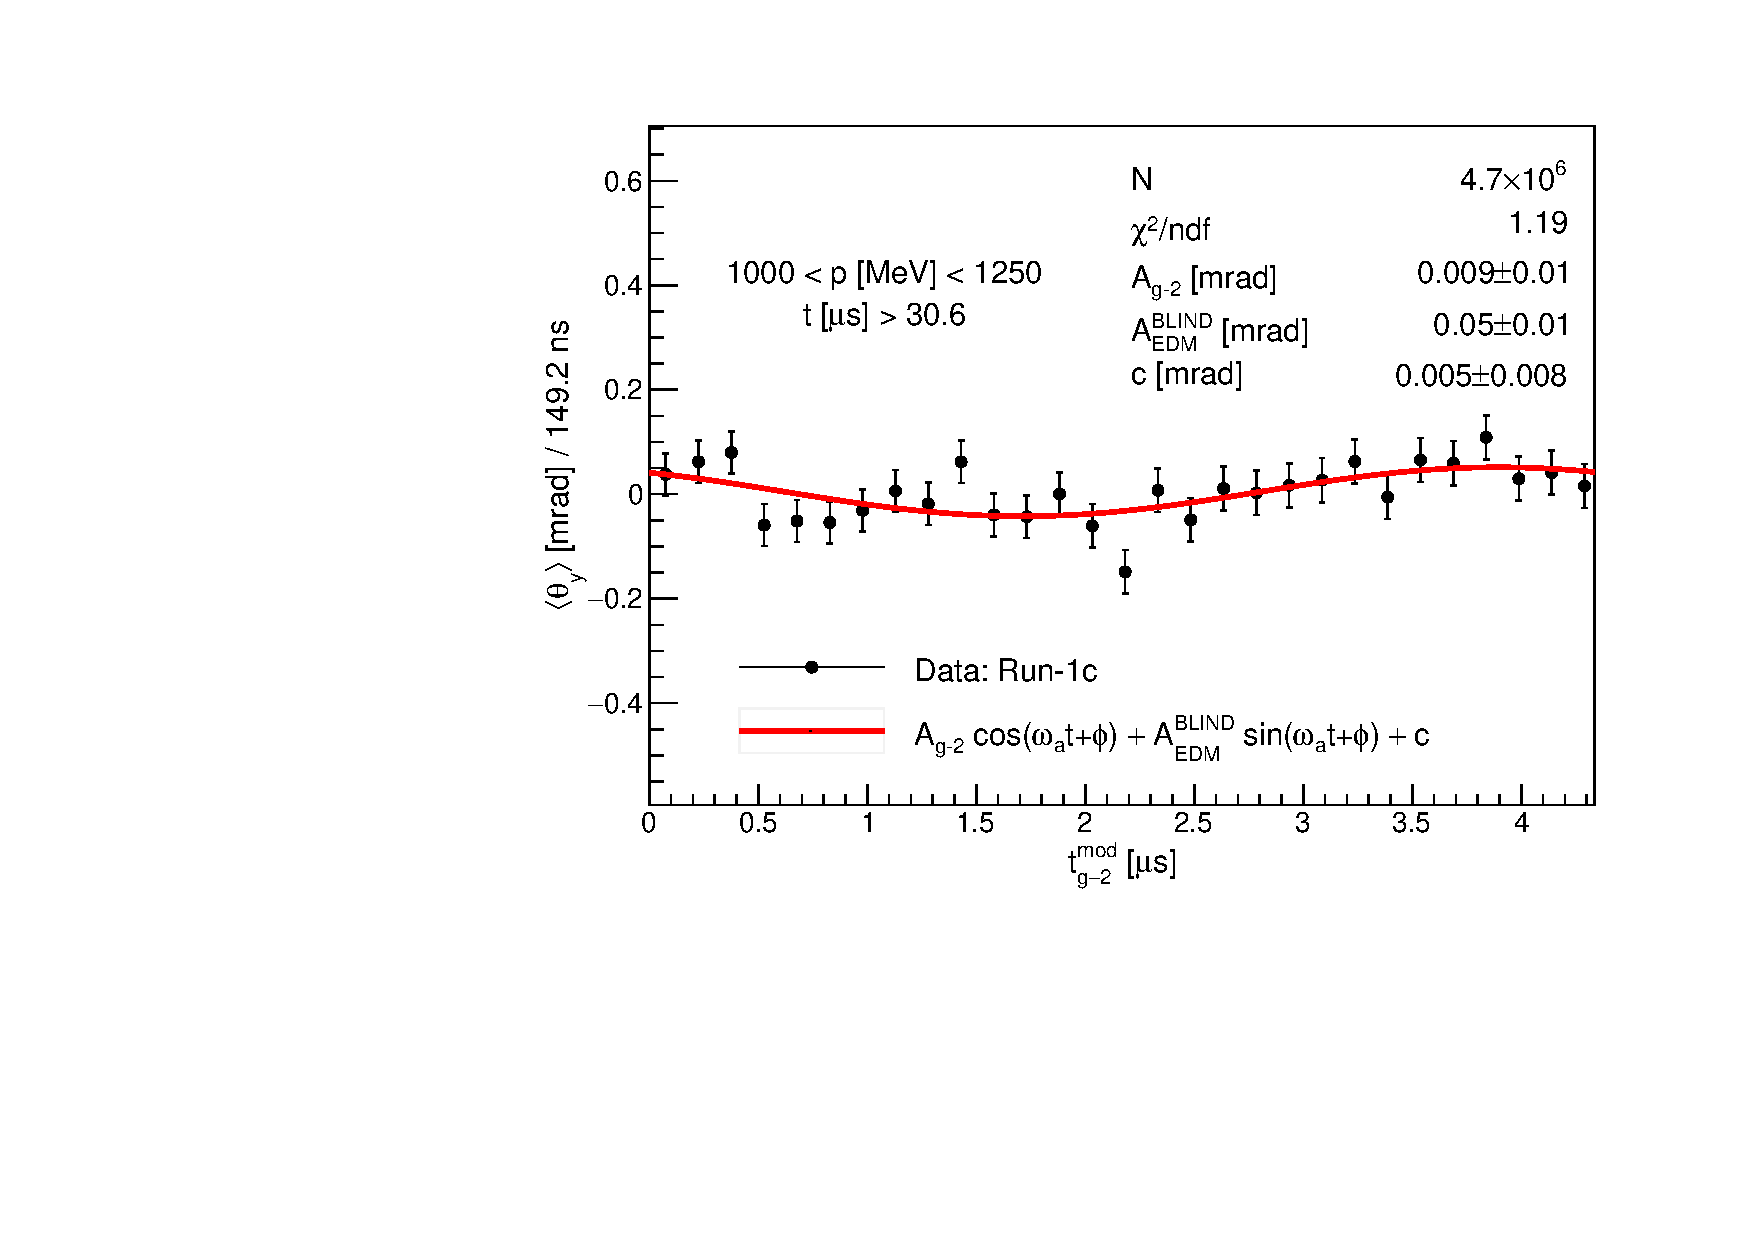
\includegraphics[trim={0 0 0 0},clip,width=.49\textwidth]{Images/Chapter6/S12S18_edmFit_1000_1250_Run-1c_250MeV_BQ.pdf}}
\subfloat[1250-1500 MeV.]{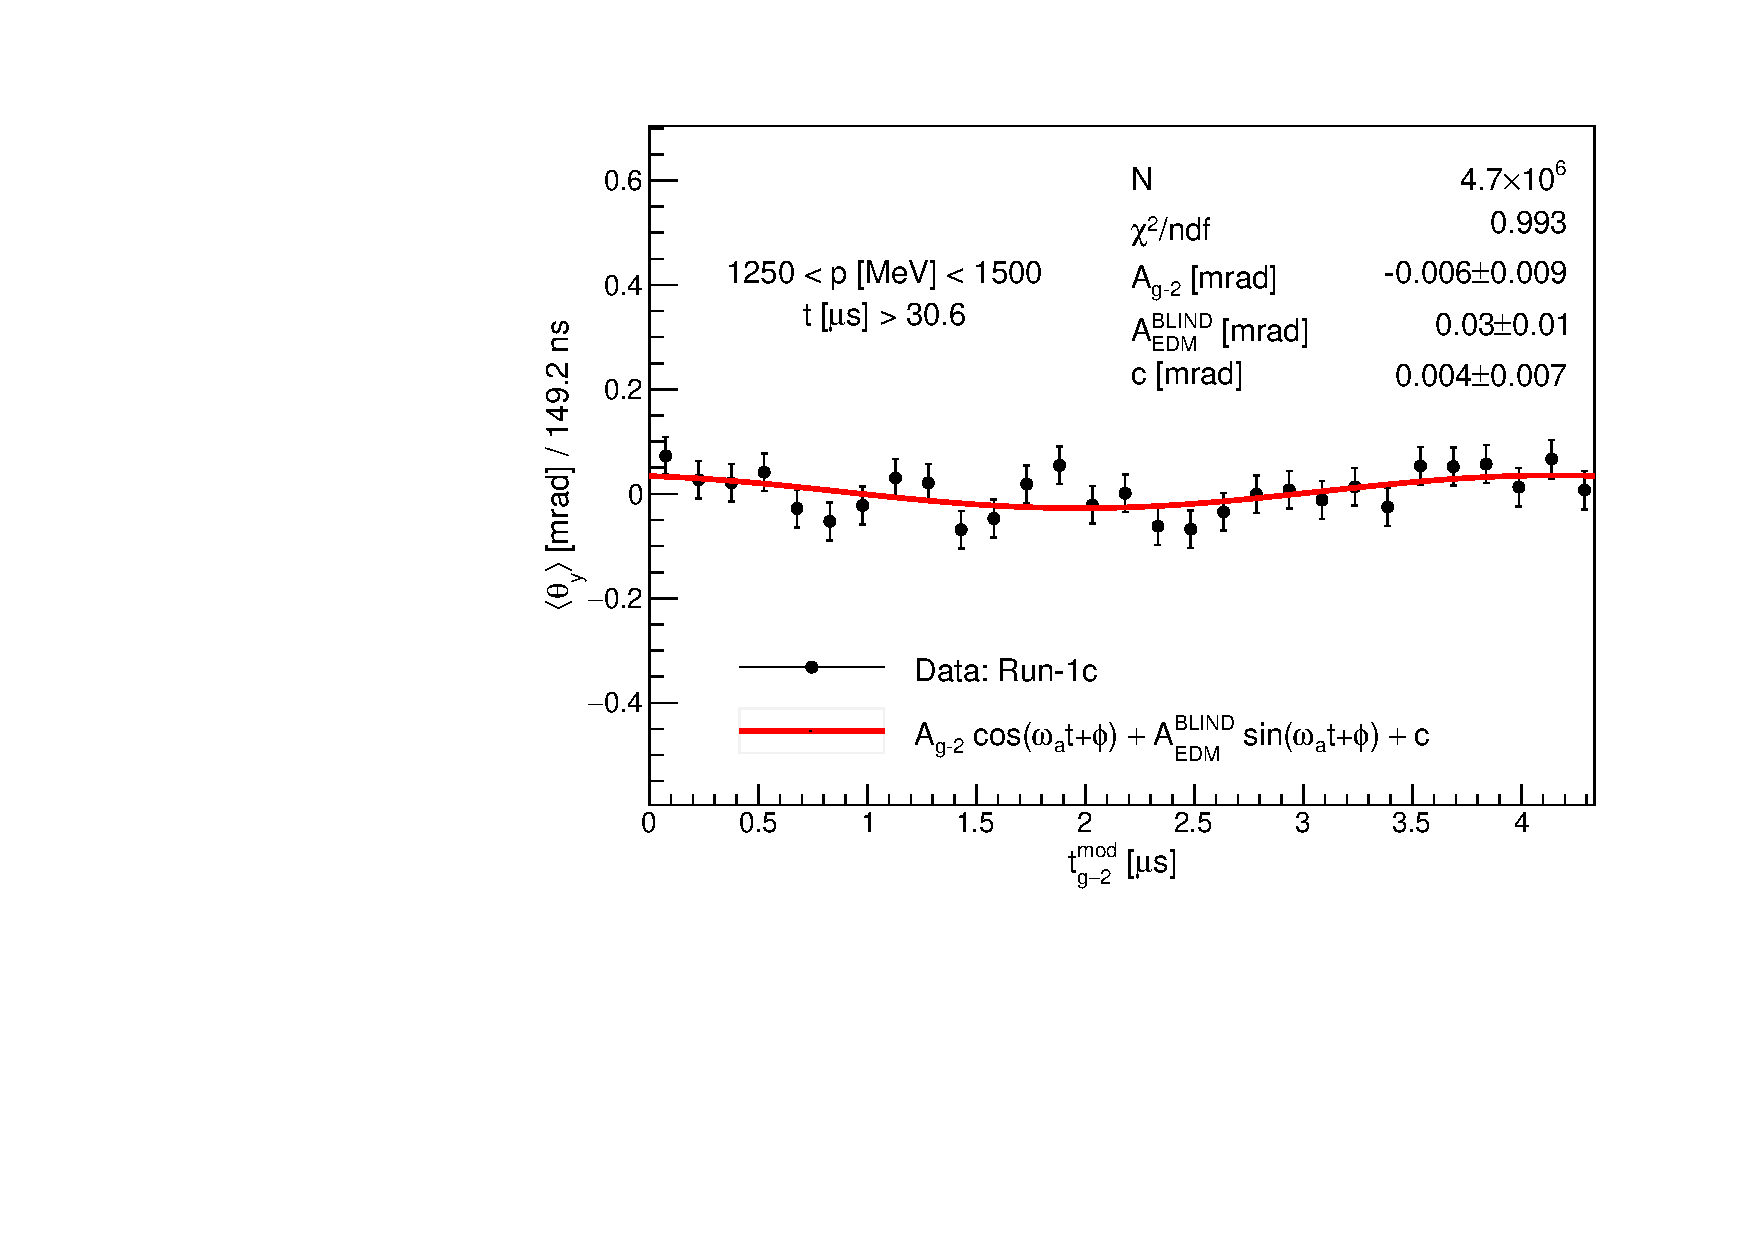
\includegraphics[trim={0 0 0 0},clip,width=.49\textwidth]{Images/Chapter6/S12S18_edmFit_1250_1500_Run-1c_250MeV_BQ.pdf}}
\hfill
\subfloat[1500-1750 MeV.]{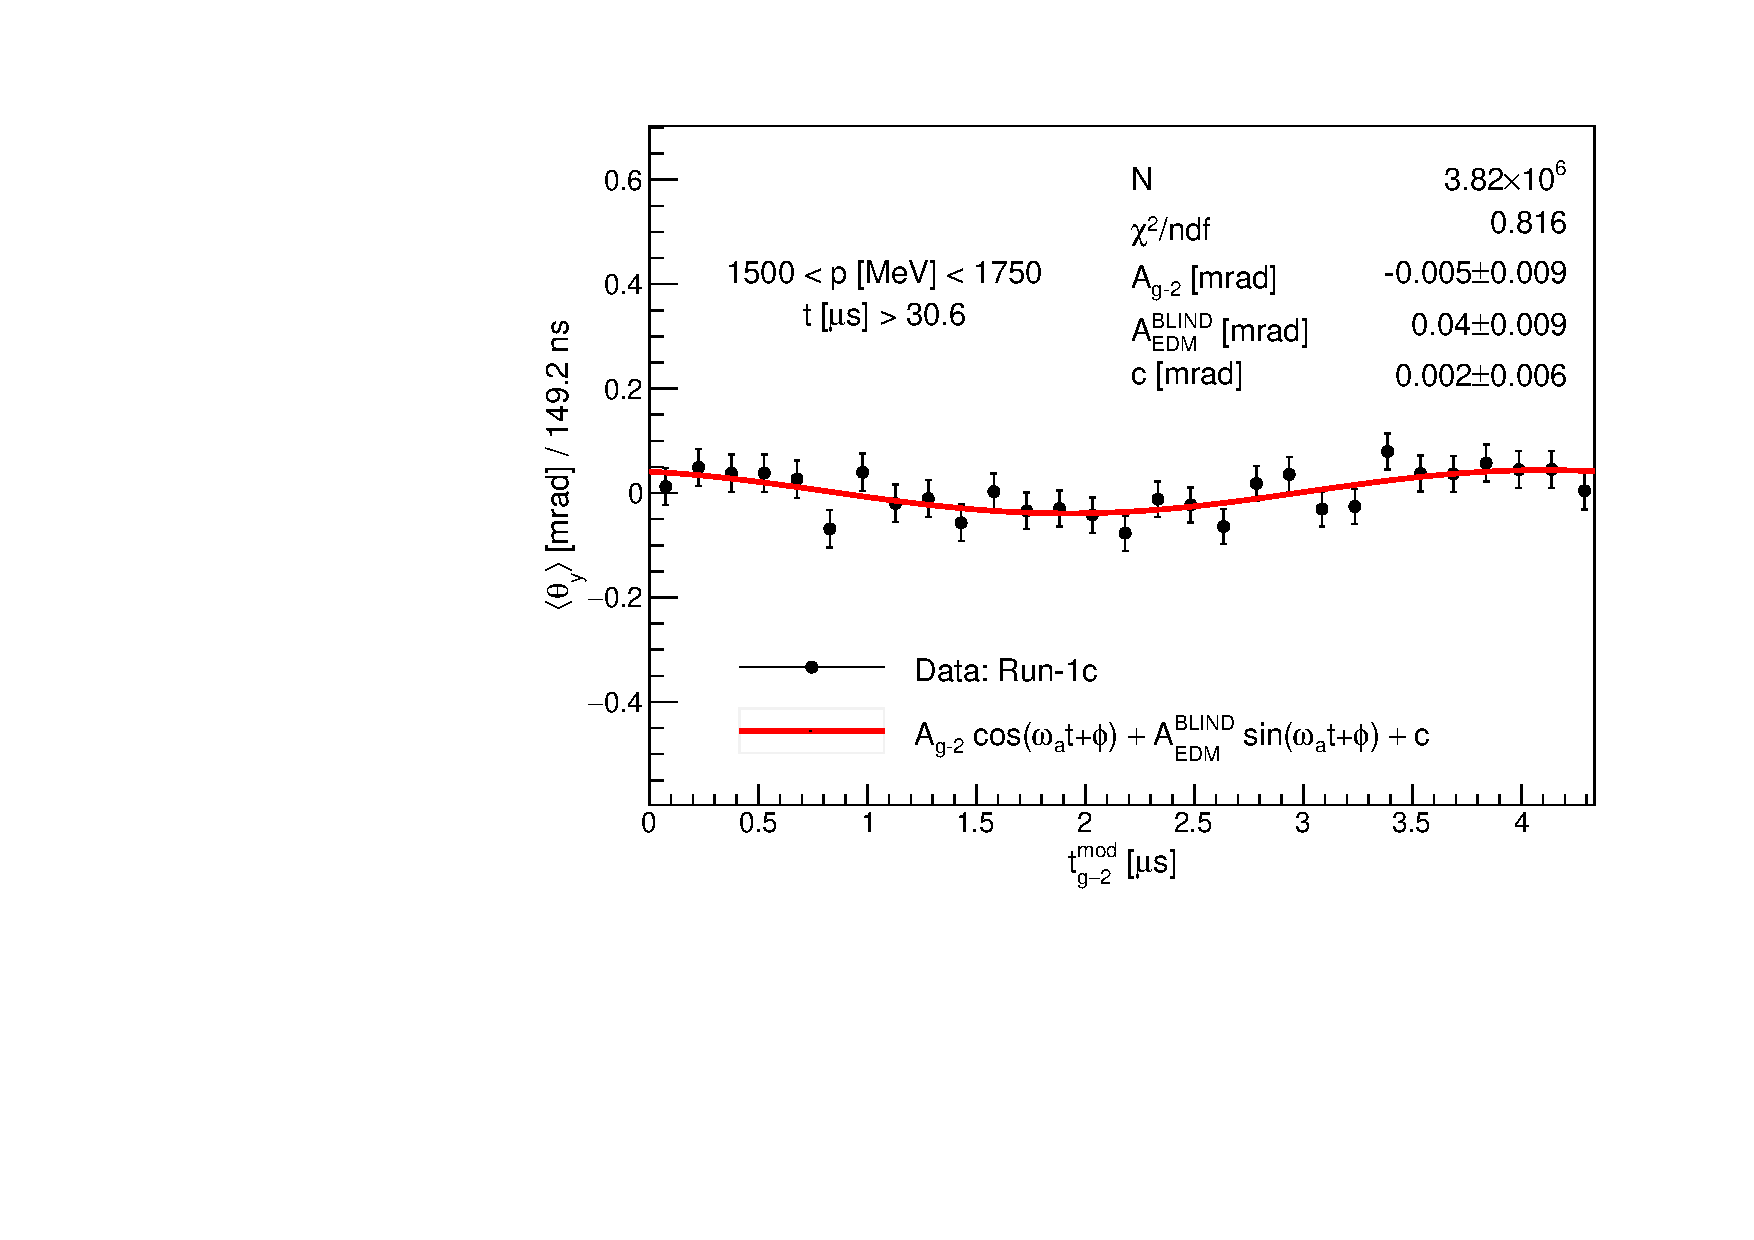
\includegraphics[trim={0 0 0 0},clip,width=.49\textwidth]{Images/Chapter6/S12S18_edmFit_1500_1750_Run-1c_250MeV_BQ.pdf}}
\subfloat[1750-2000 MeV.]{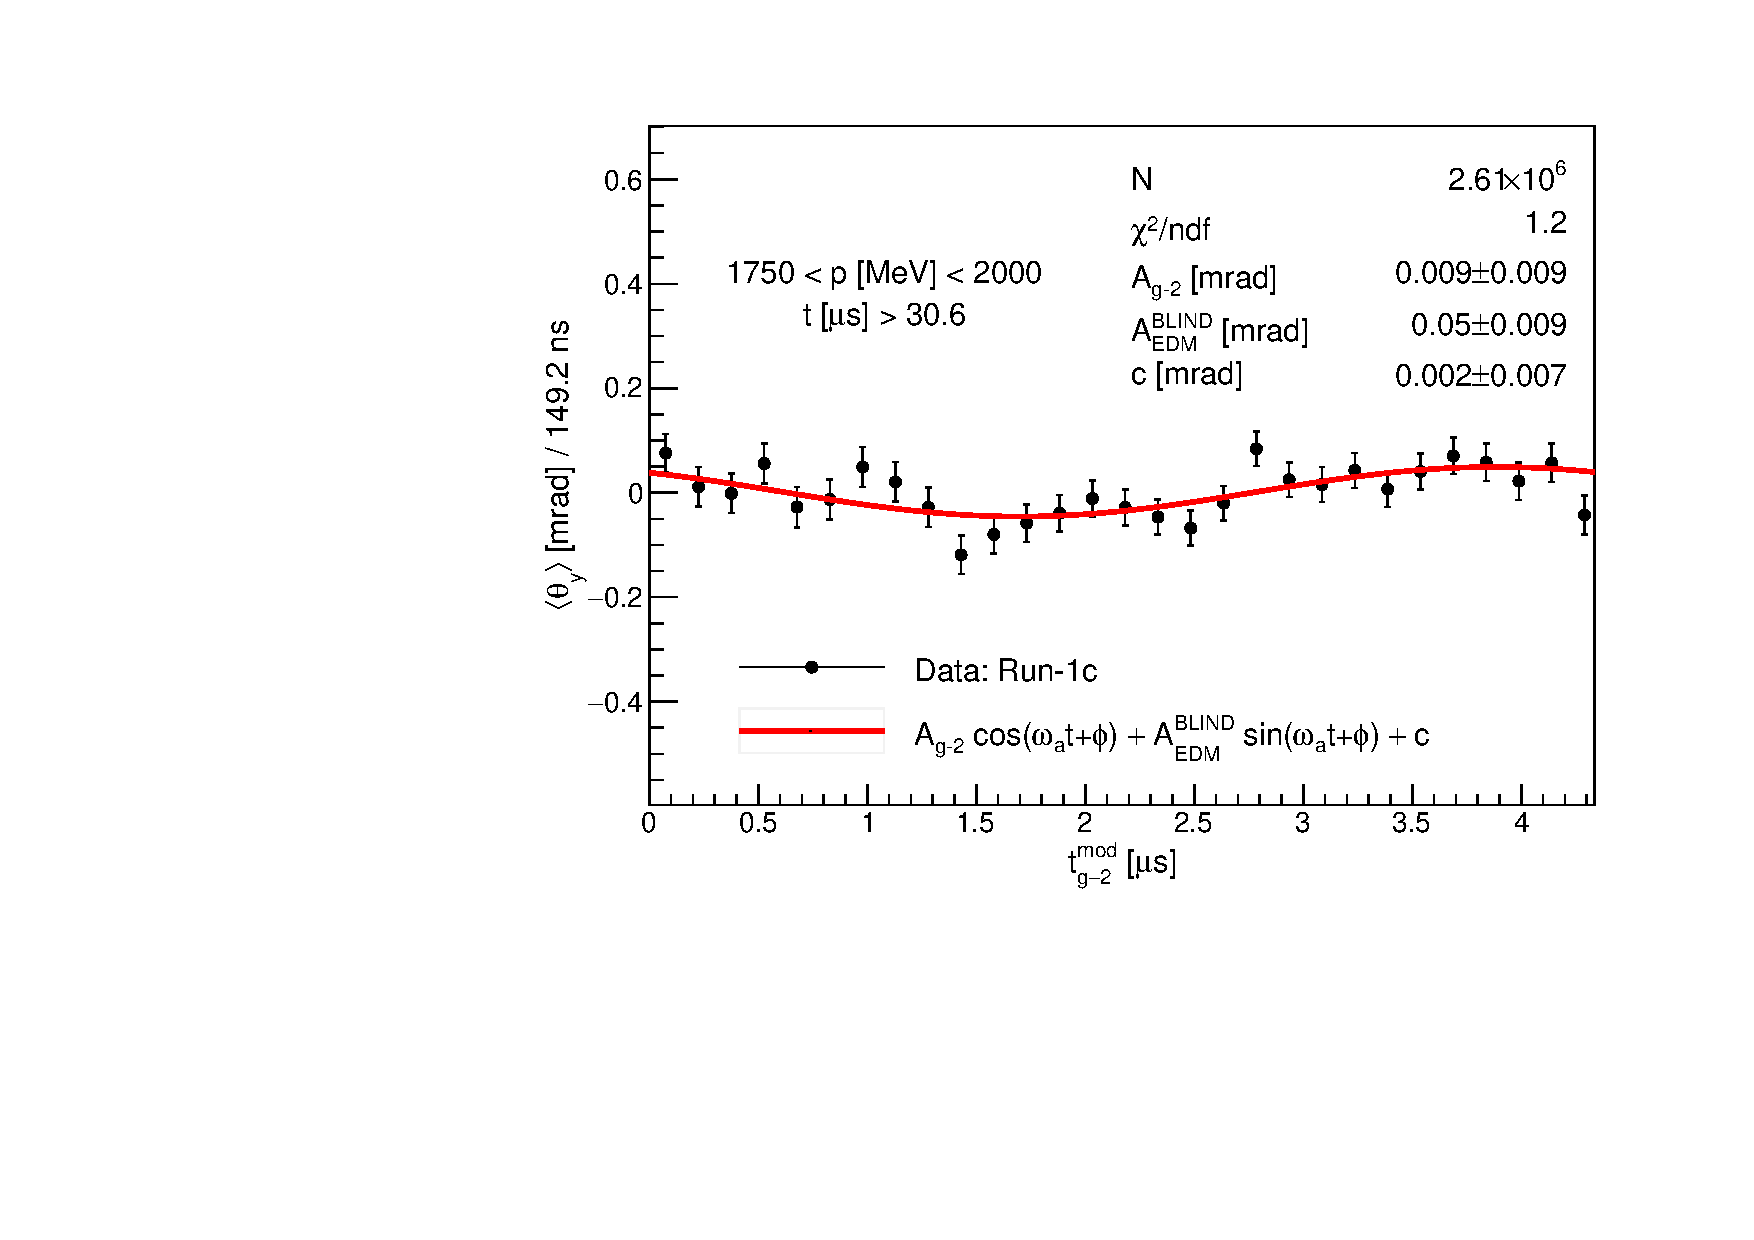
\includegraphics[trim={0 0 0 0},clip,width=.49\textwidth]{Images/Chapter6/S12S18_edmFit_1750_2000_Run-1c_250MeV_BQ.pdf}}
\hfill
\subfloat[2000-2250 MeV.]{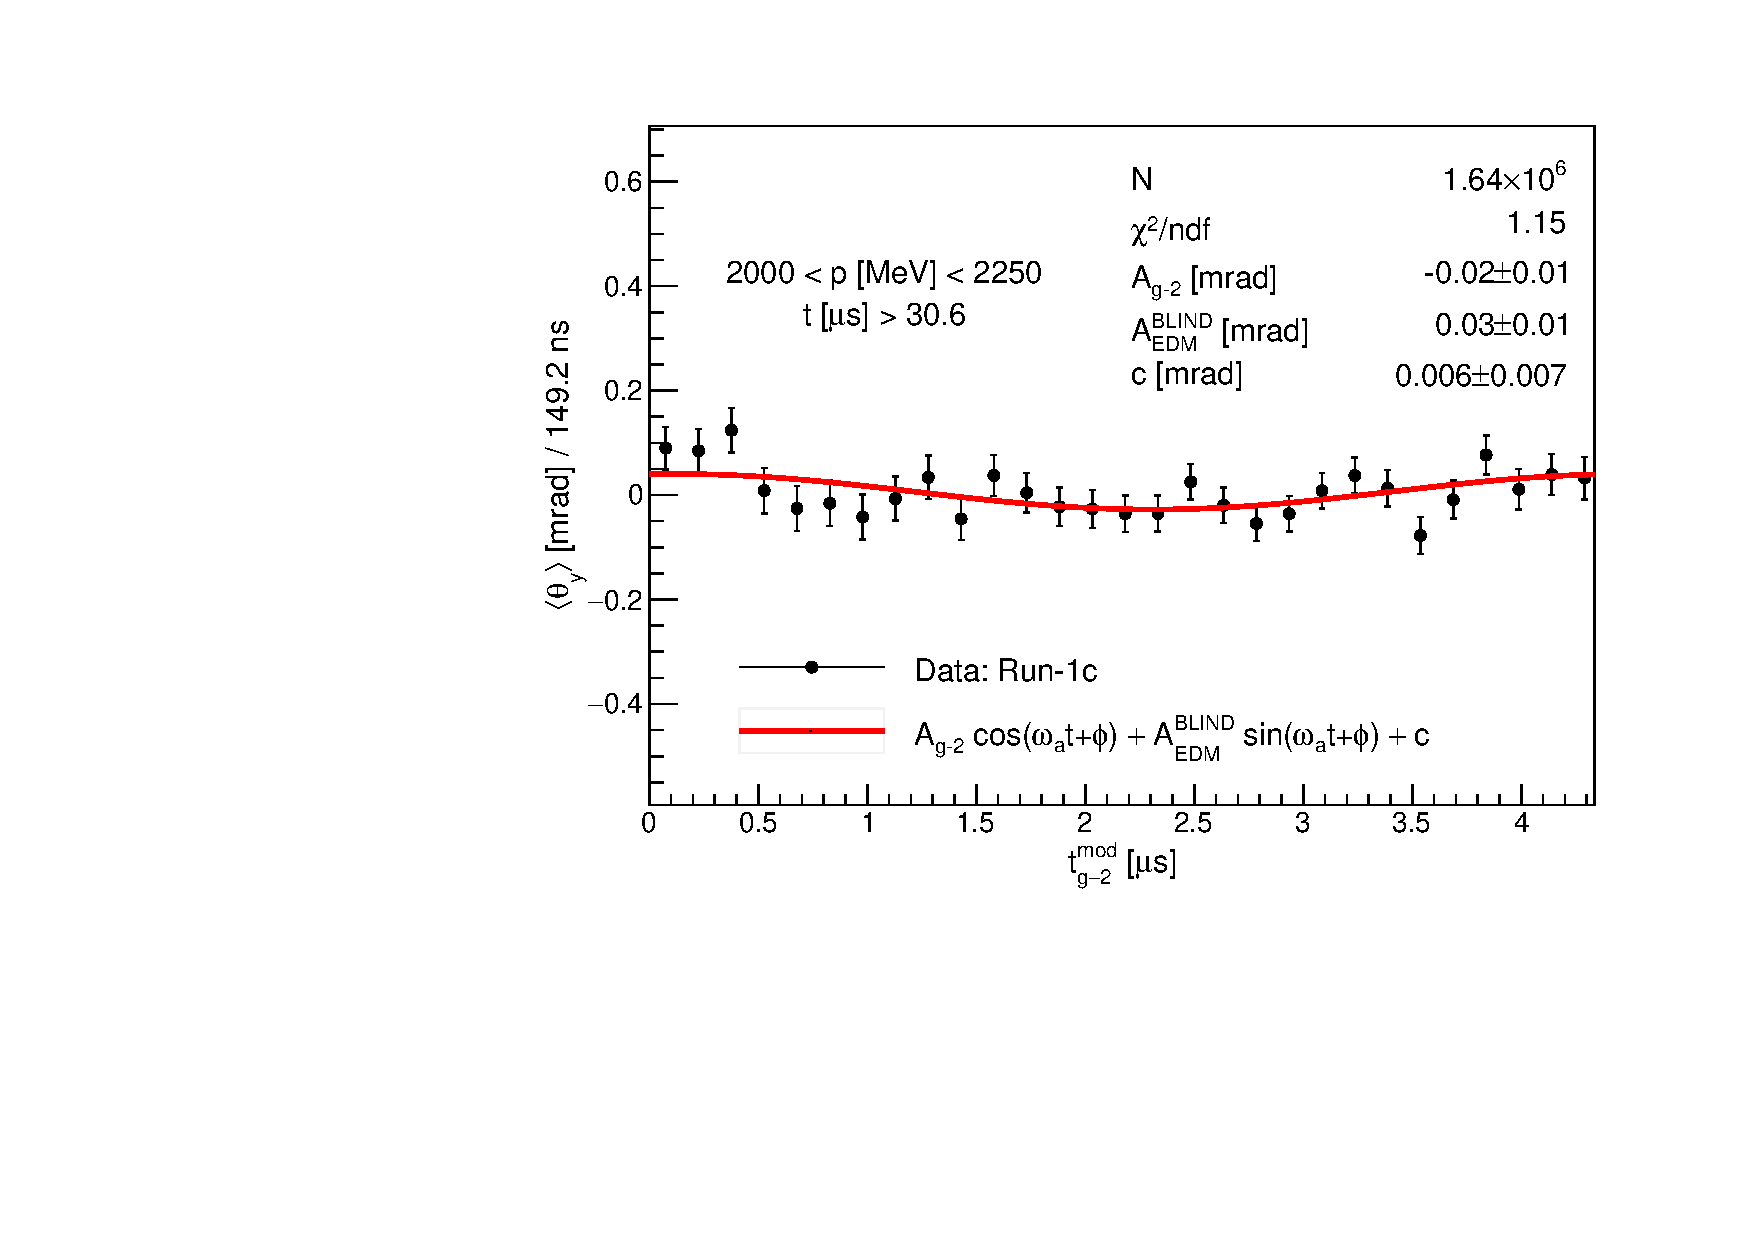
\includegraphics[trim={0 0 0 0},clip,width=.49\textwidth]{Images/Chapter6/S12S18_edmFit_2000_2250_Run-1c_250MeV_BQ.pdf}}
\subfloat[2250-2500 MeV.]{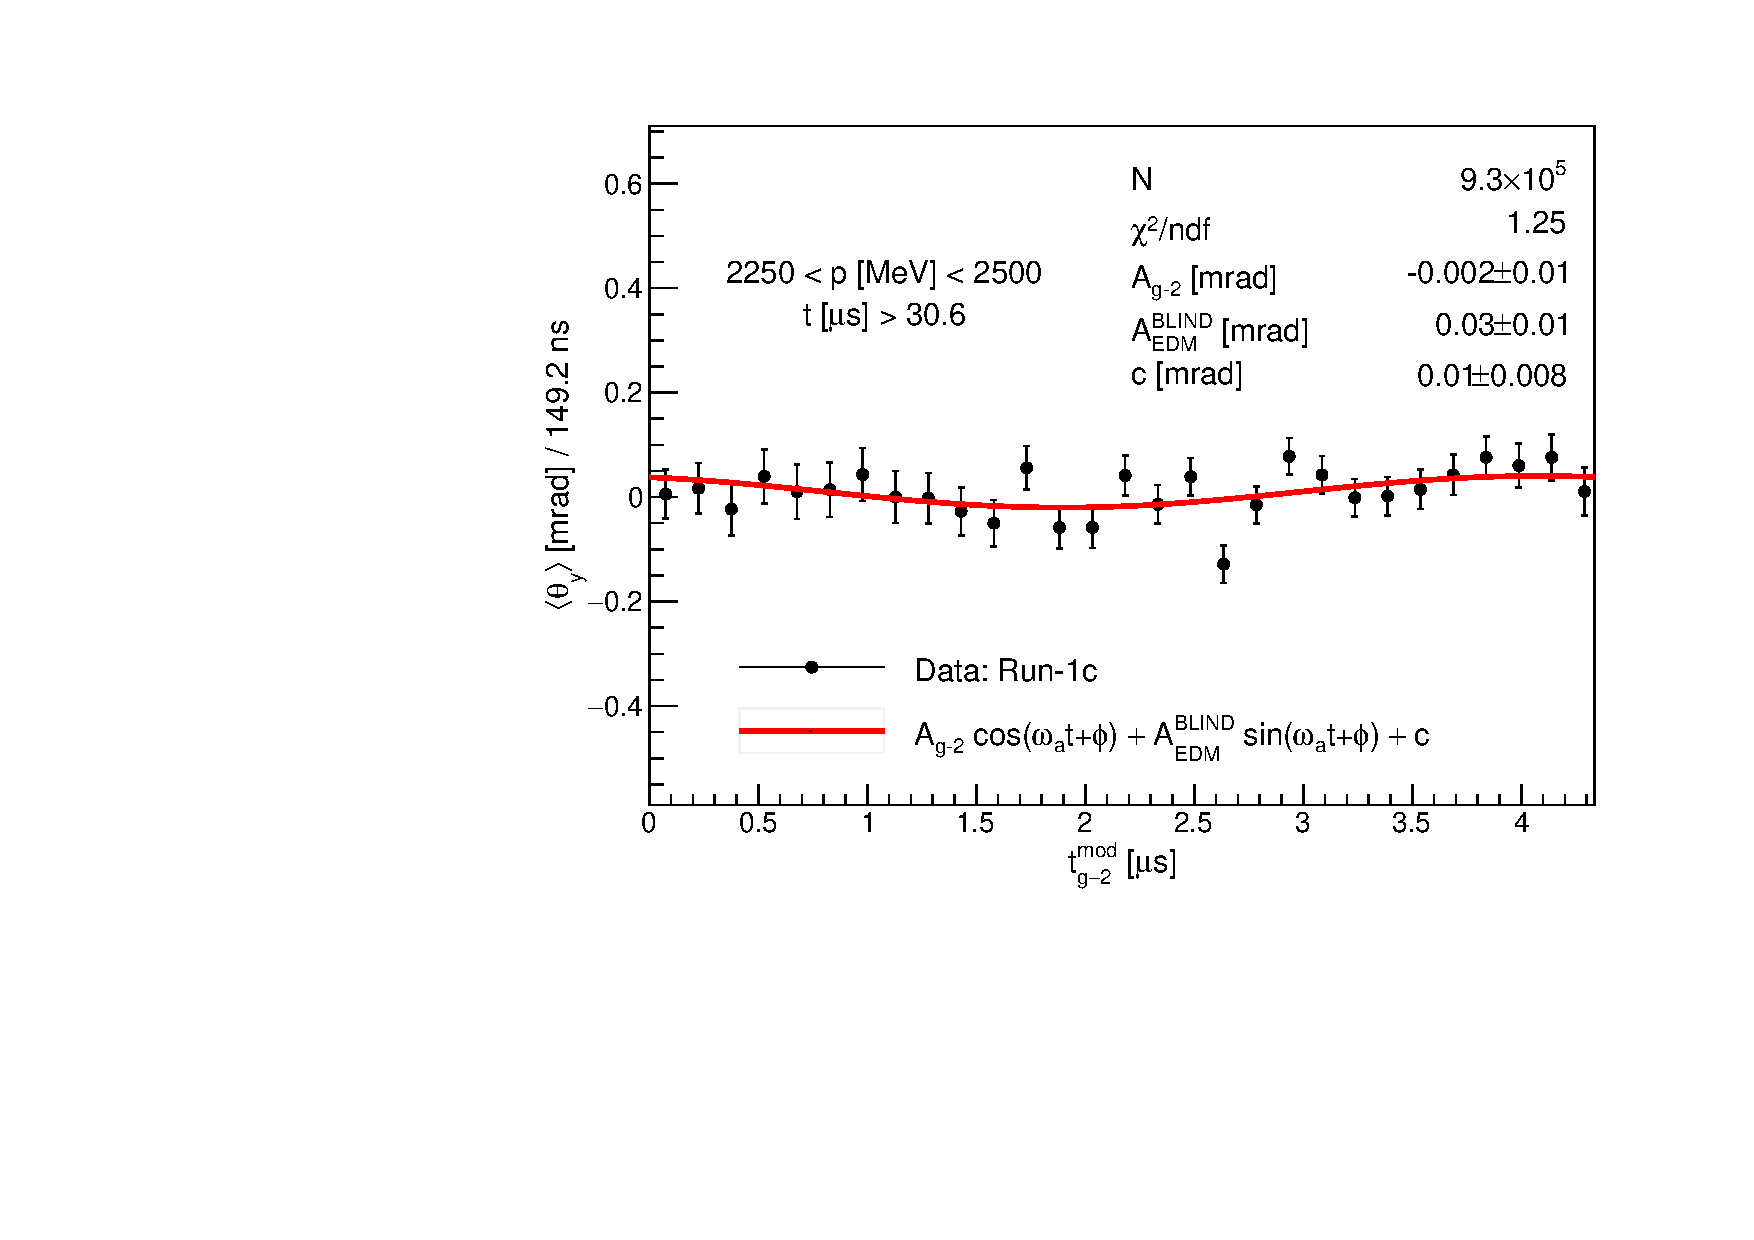
\includegraphics[trim={0 0 0 0},clip,width=.49\textwidth]{Images/Chapter6/S12S18_edmFit_2250_2500_Run-1c_250MeV_BQ.pdf}}
\caption{Momentum-binned vertical angle oscillation fits for Run-1c. Tracker stations 12 and 18 are combined.}
\label{fig:Run1cMomBinnedFits}
\end{figure}
\clearpage

\begin{figure}[]
\centering{}
\subfloat[1000-1250 MeV.]{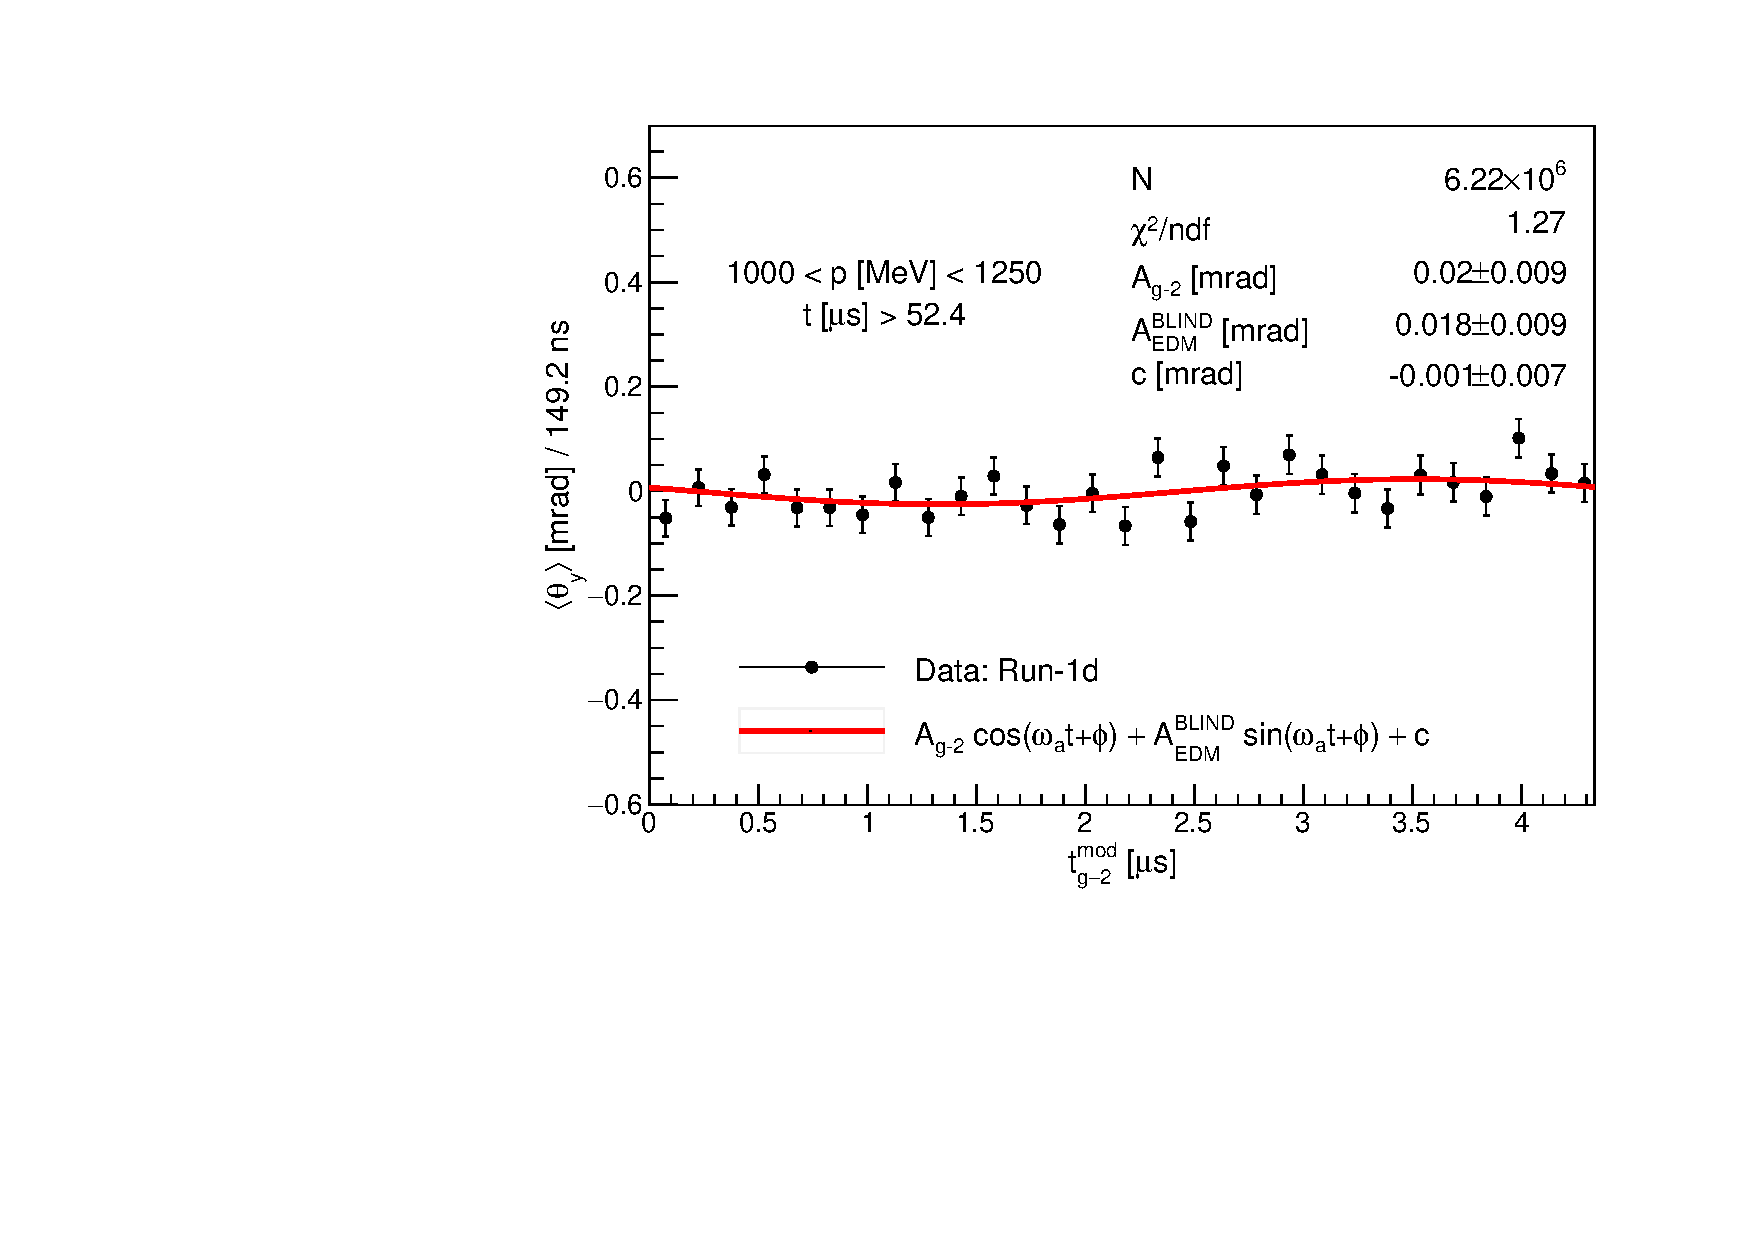
\includegraphics[trim={0 0 0 0},clip,width=.49\textwidth]{Images/Chapter6/S12S18_edmFit_1000_1250_Run-1d_250MeV_BQ.pdf}}
\subfloat[1250-1500 MeV.]{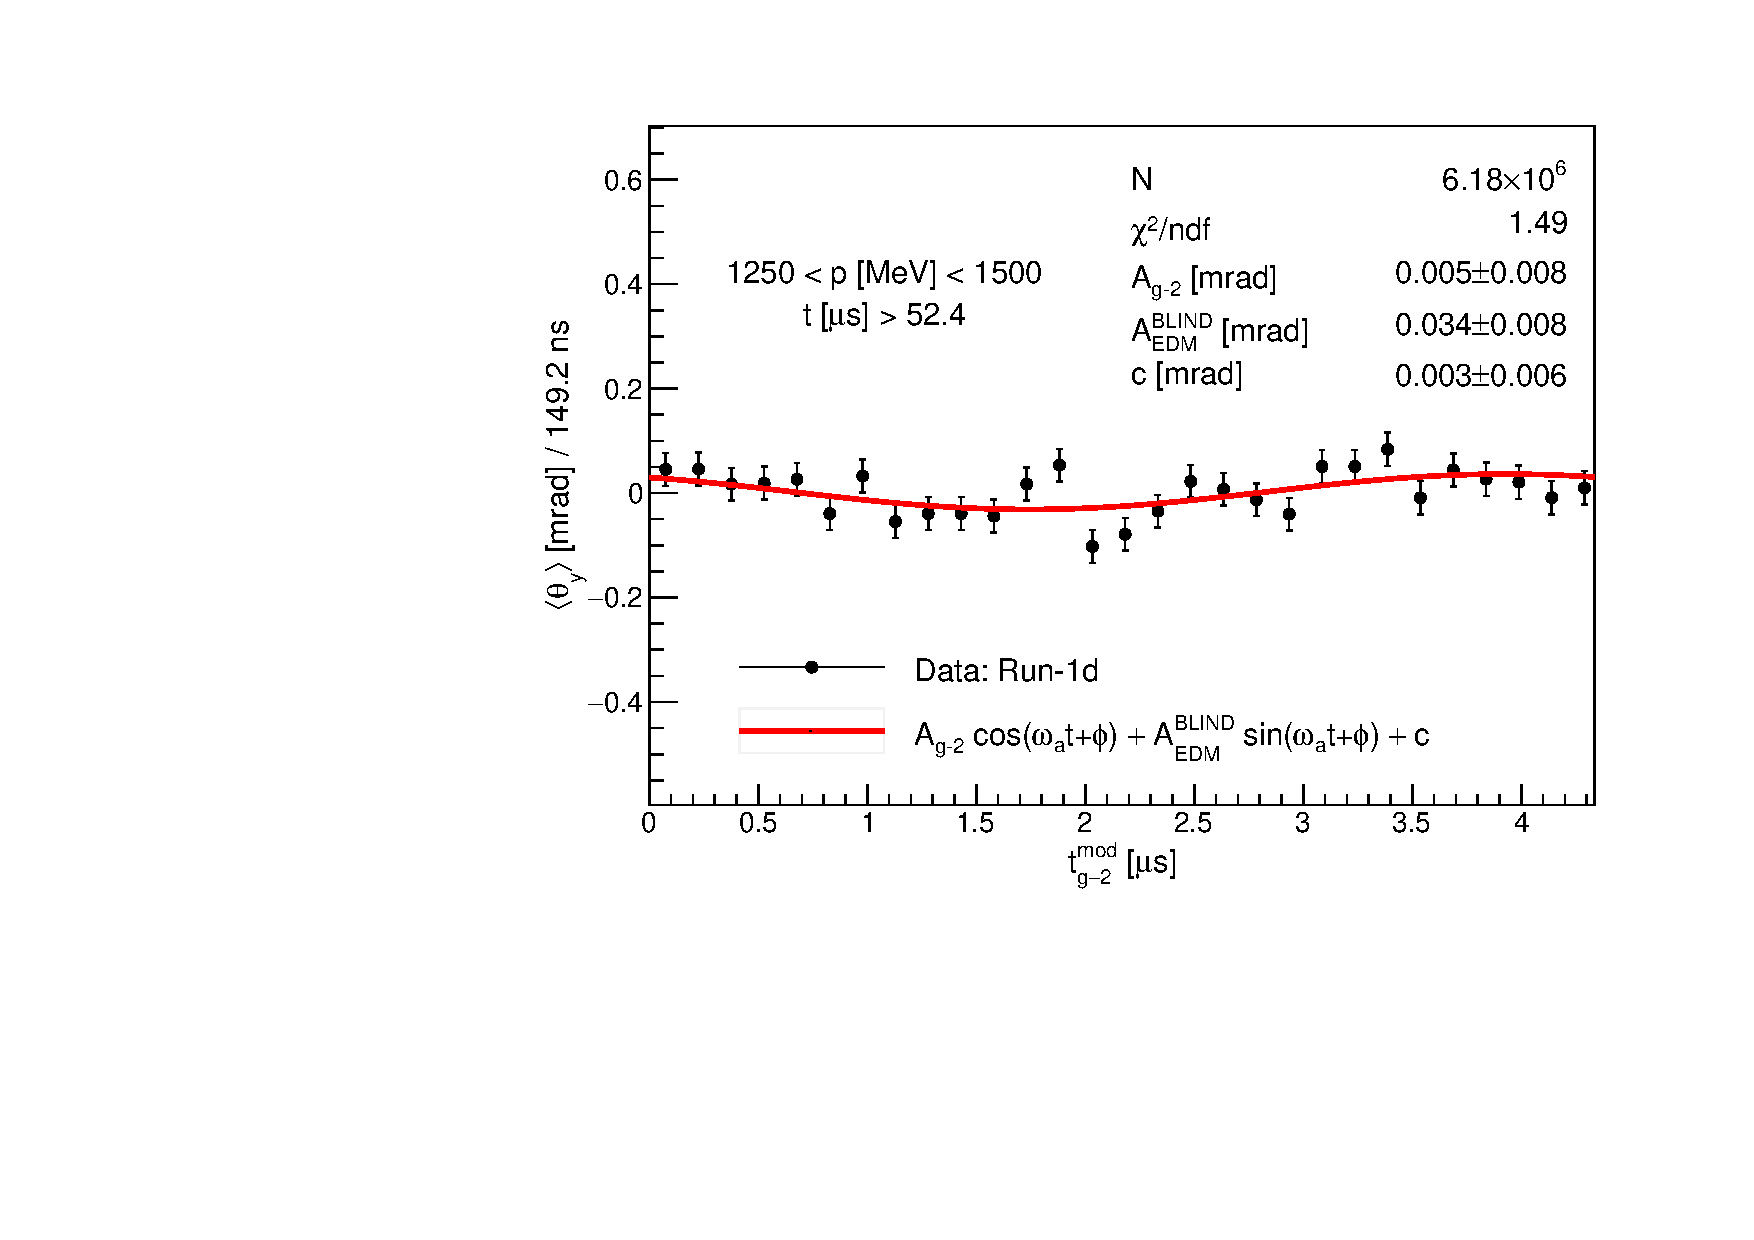
\includegraphics[trim={0 0 0 0},clip,width=.49\textwidth]{Images/Chapter6/S12S18_edmFit_1250_1500_Run-1d_250MeV_BQ.pdf}}
\hfill
\subfloat[1500-1750 MeV.]{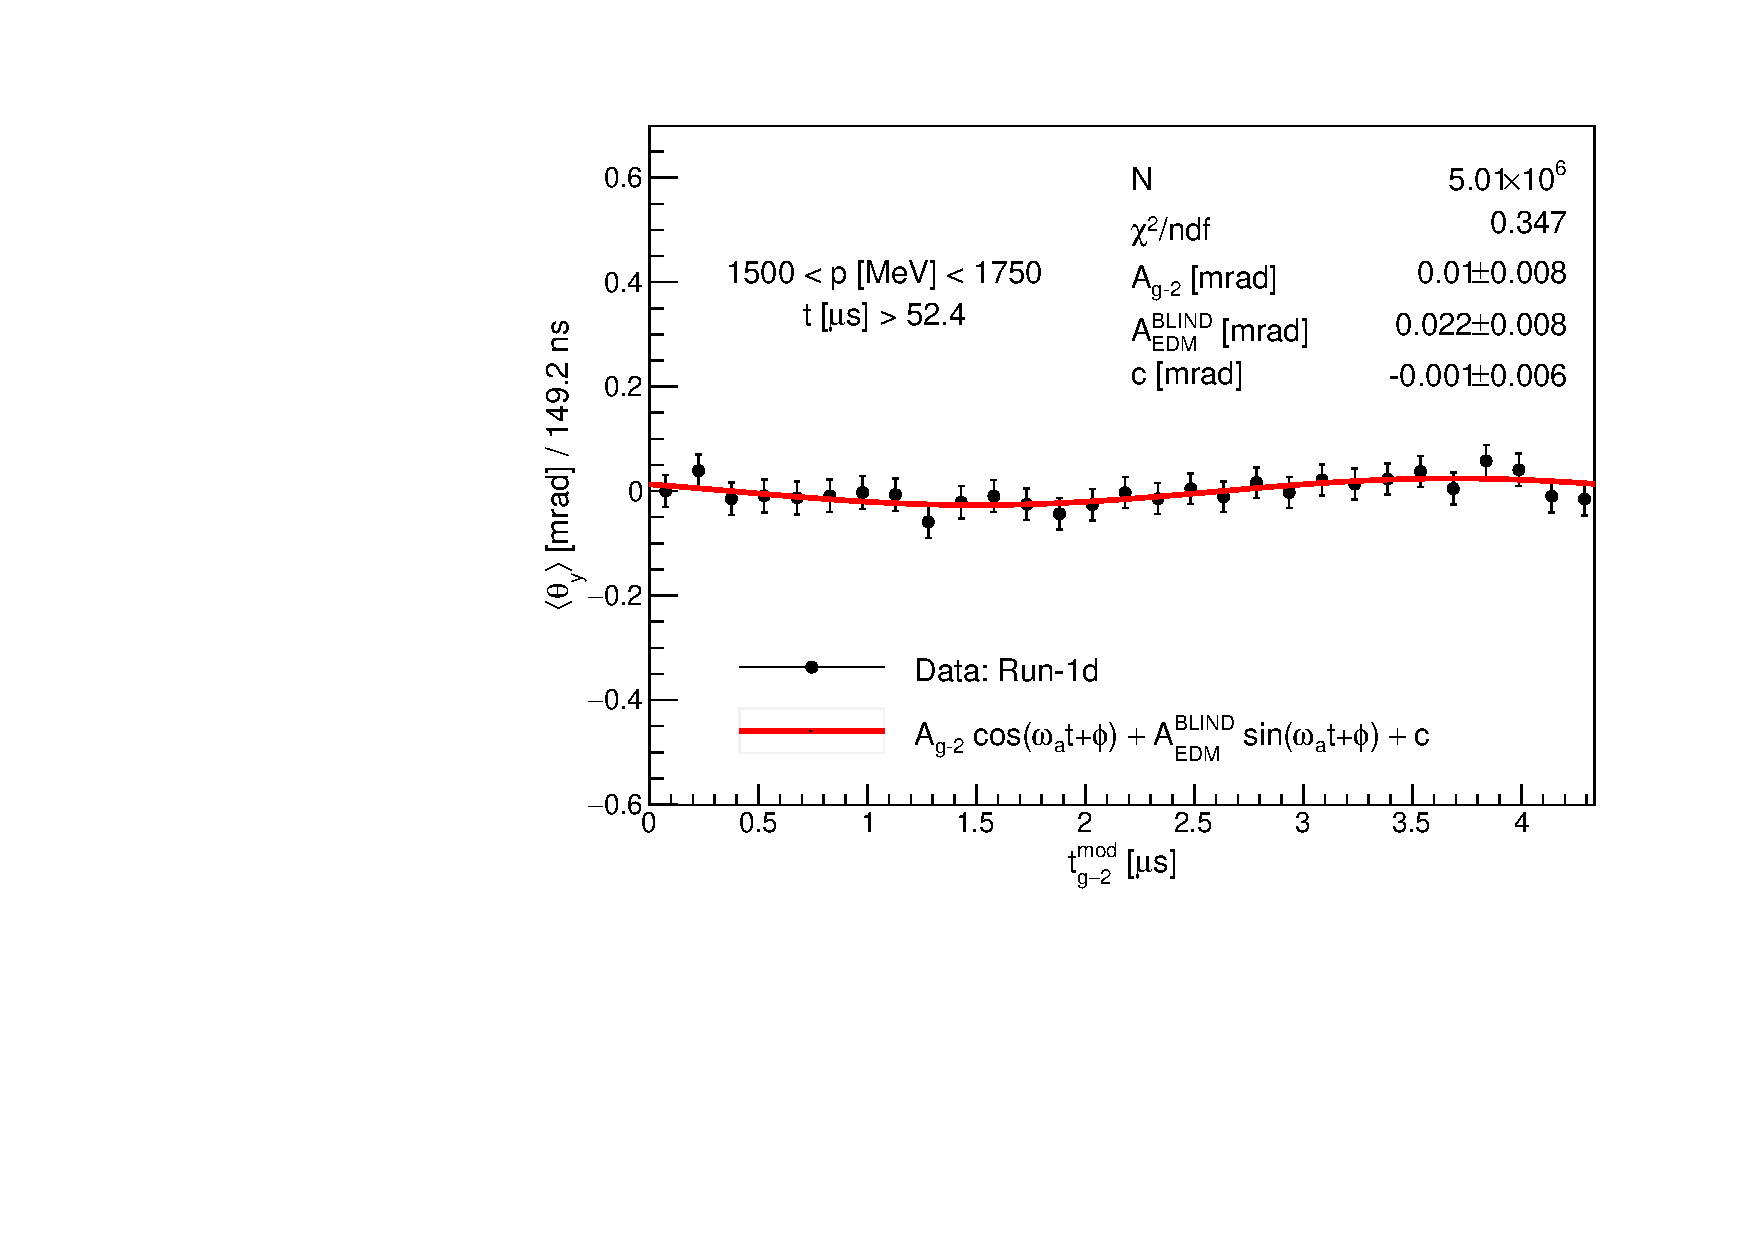
\includegraphics[trim={0 0 0 0},clip,width=.49\textwidth]{Images/Chapter6/S12S18_edmFit_1500_1750_Run-1d_250MeV_BQ.pdf}}
\subfloat[1750-2000 MeV.]{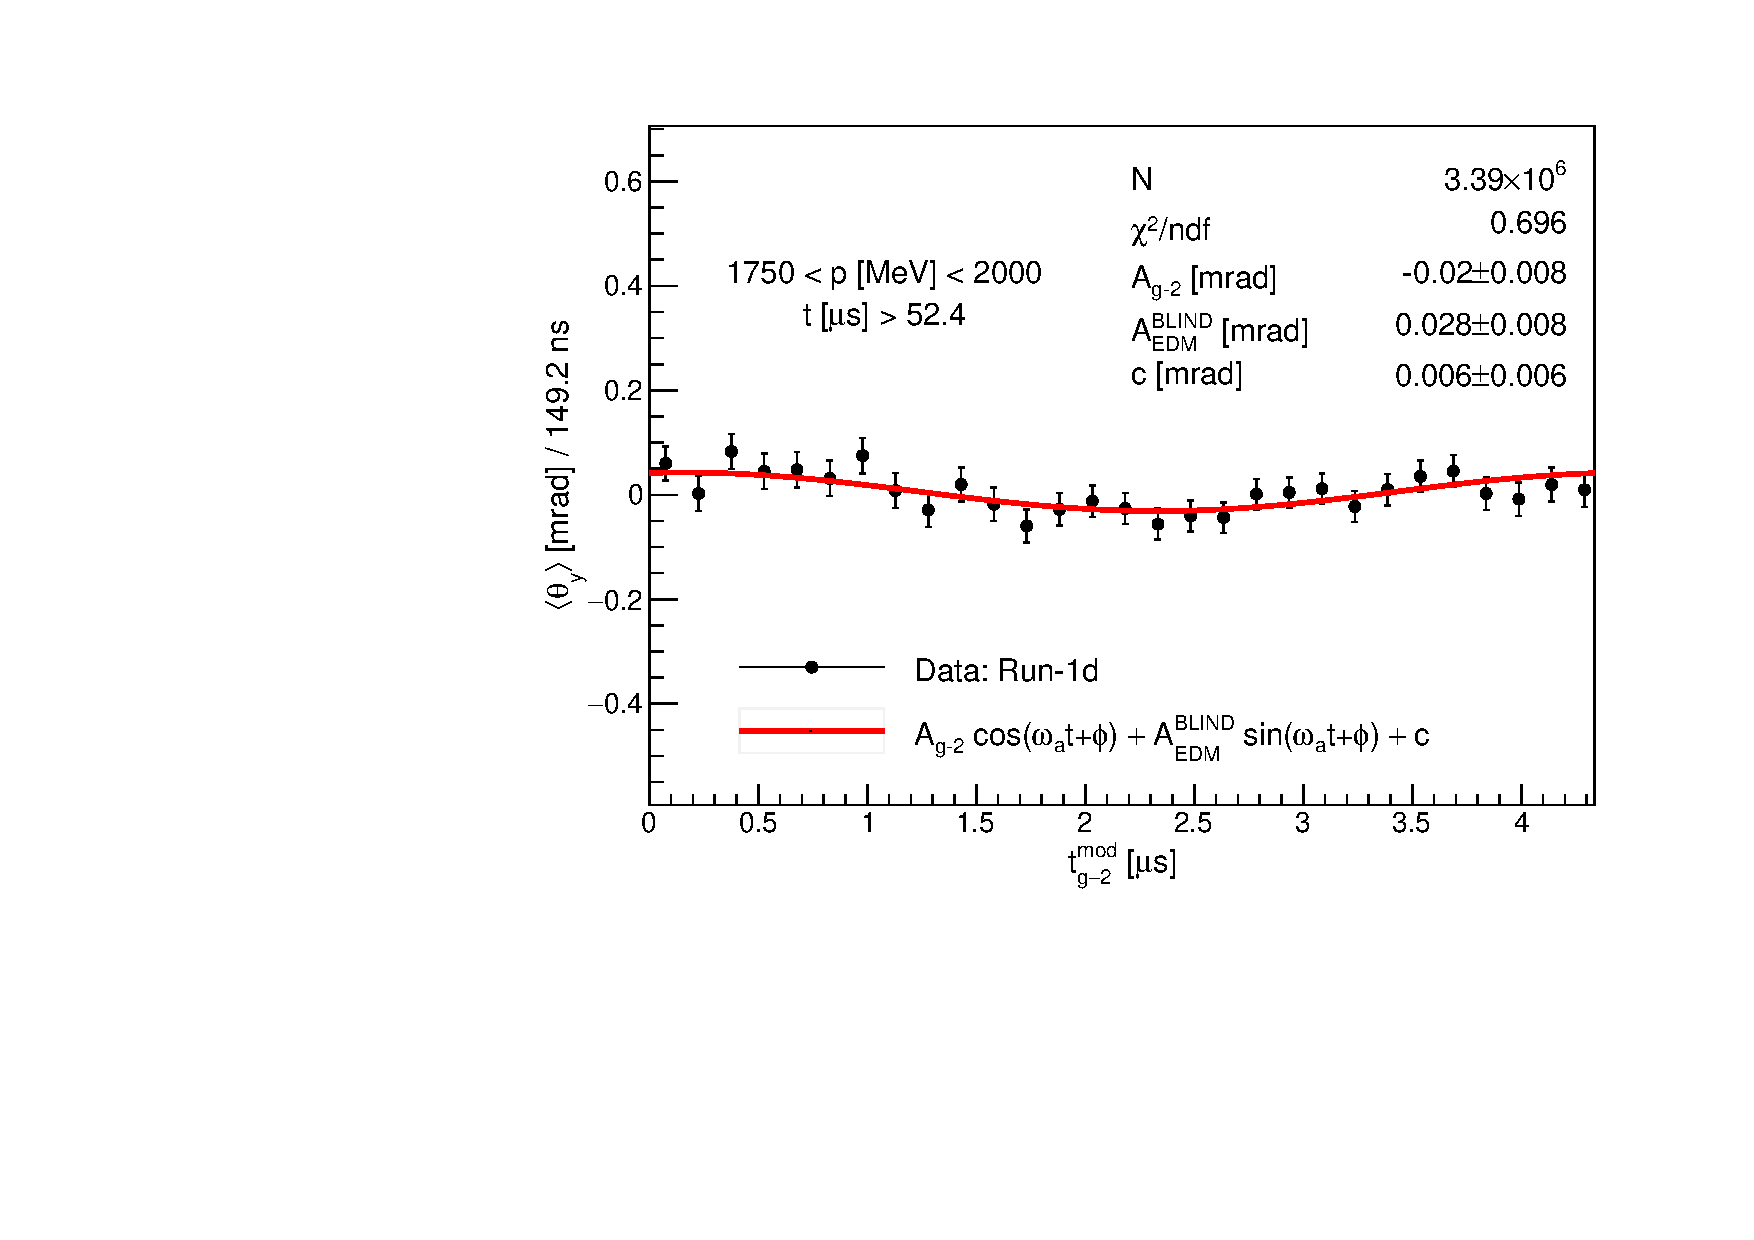
\includegraphics[trim={0 0 0 0},clip,width=.49\textwidth]{Images/Chapter6/S12S18_edmFit_1750_2000_Run-1d_250MeV_BQ.pdf}}
\hfill
\subfloat[2000-2250 MeV.]{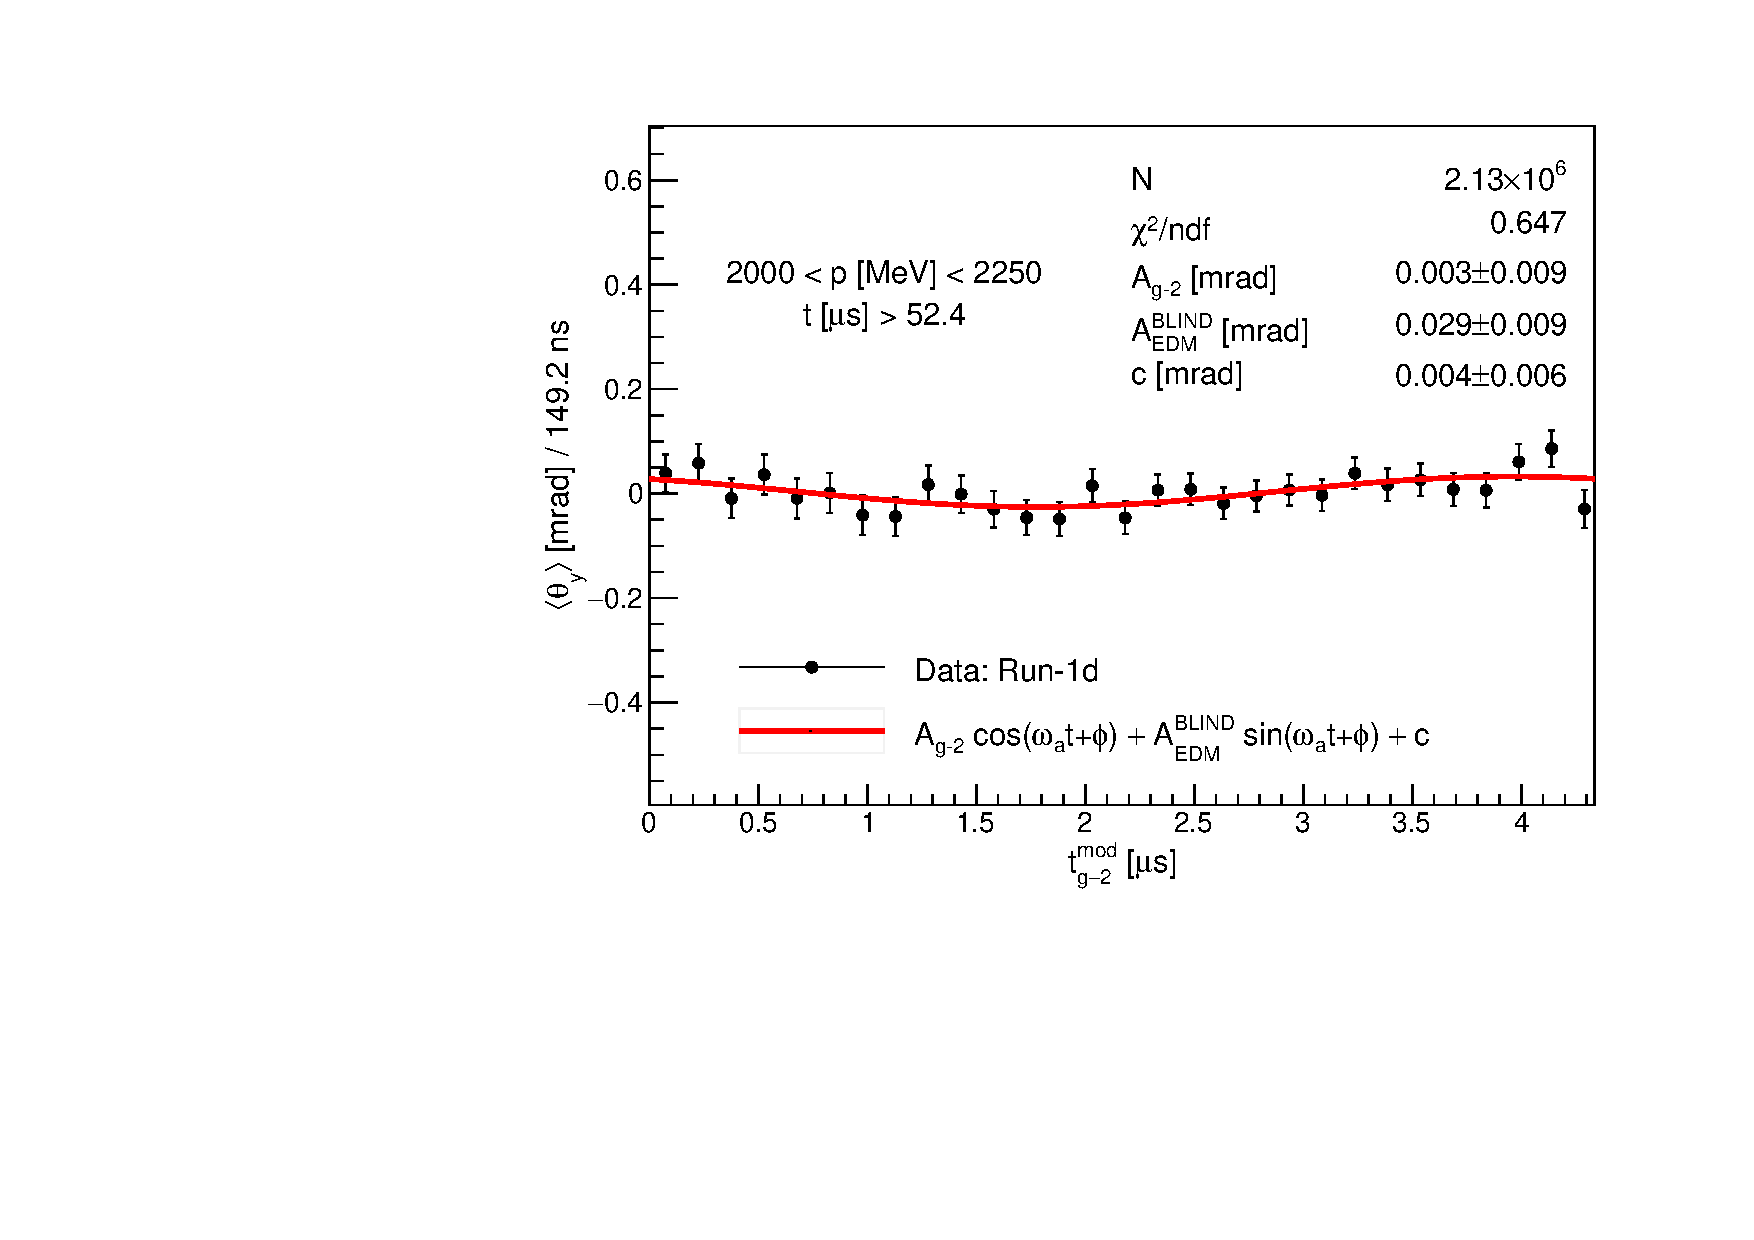
\includegraphics[trim={0 0 0 0},clip,width=.49\textwidth]{Images/Chapter6/S12S18_edmFit_2000_2250_Run-1d_250MeV_BQ.pdf}}
\subfloat[2250-2500 MeV.]{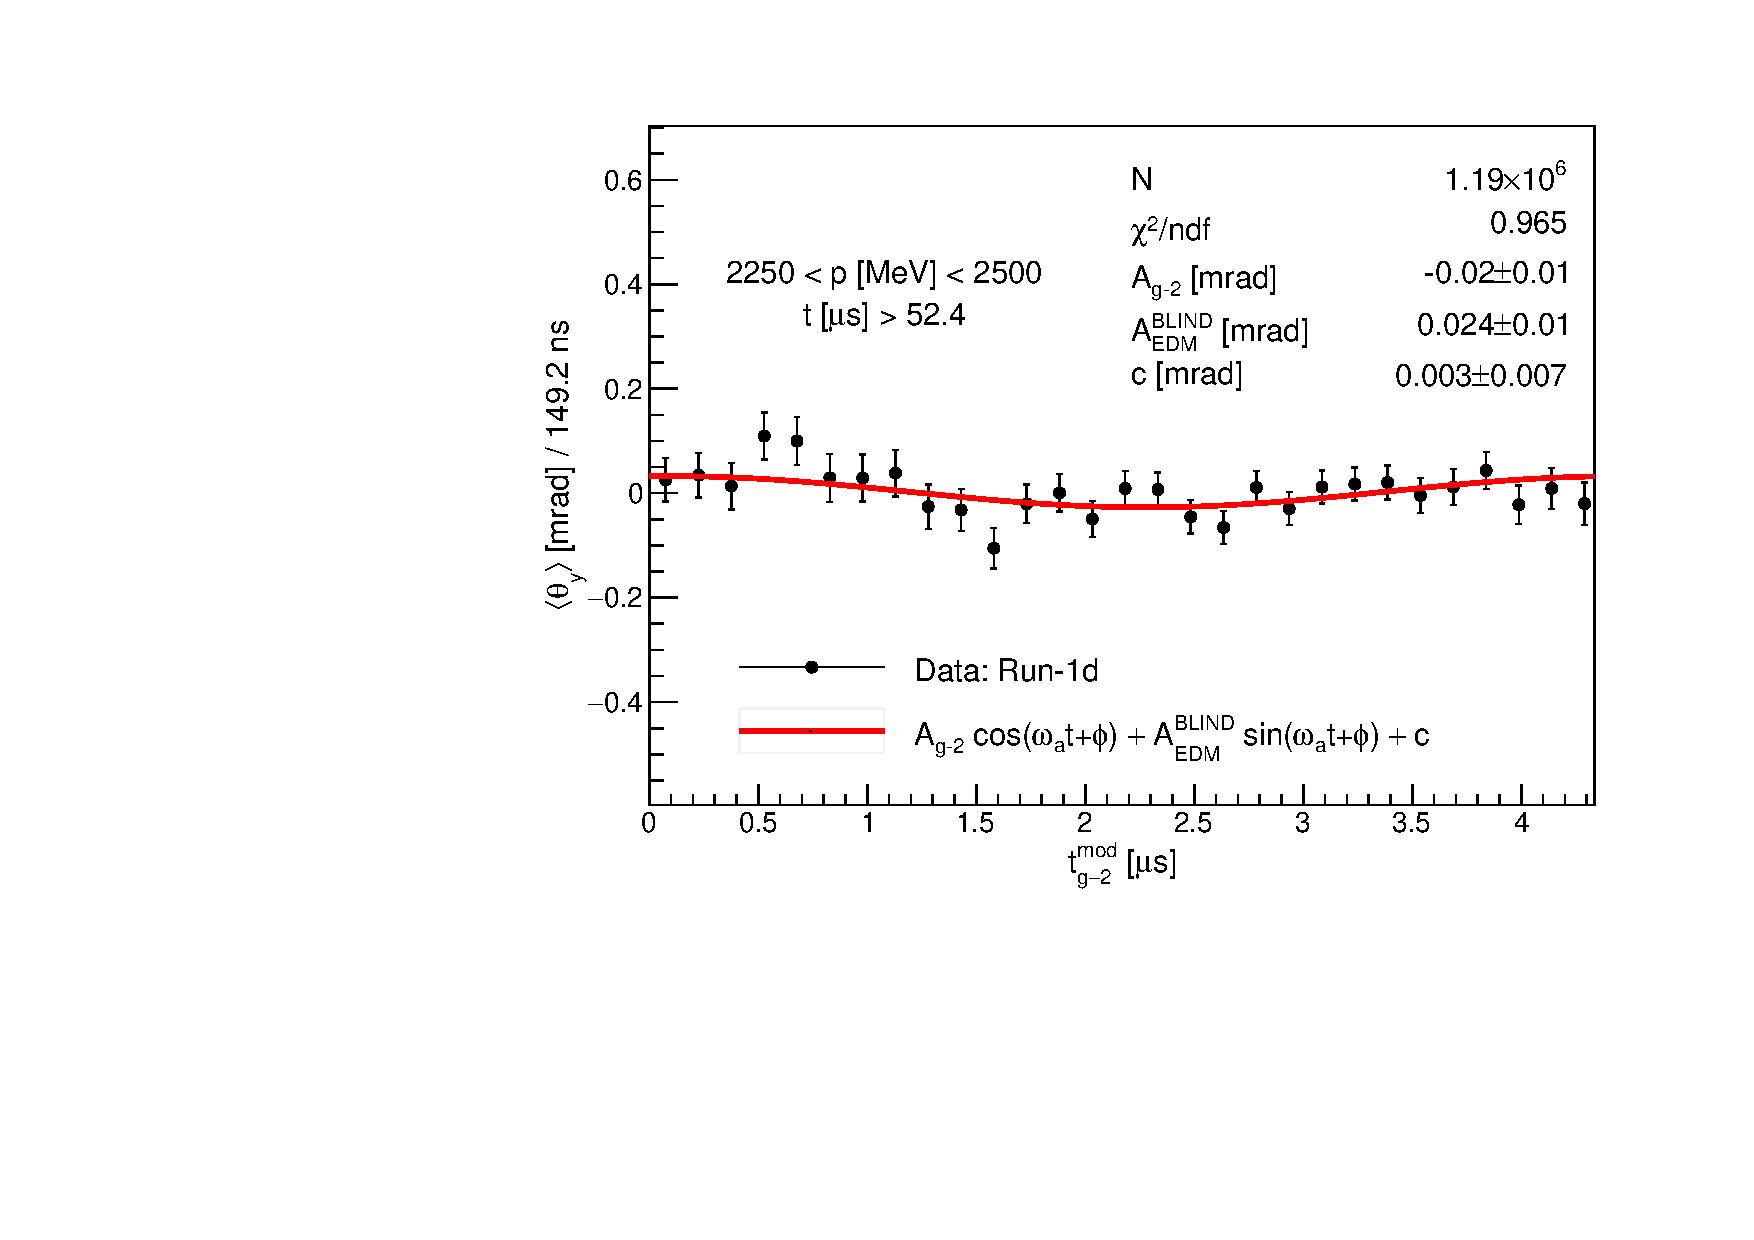
\includegraphics[trim={0 0 0 0},clip,width=.49\textwidth]{Images/Chapter6/S12S18_edmFit_2250_2500_Run-1d_250MeV_BQ.pdf}}
\caption{Momentum-binned vertical angle oscillation fits for Run-1d. Tracker stations 12 and 18 are combined.}
\label{fig:Run1dMomBinnedFits}
\end{figure}
\clearpage

% \clearpage  

\subsection{Extracting the tilt angle}\label{sec:ExtractTiltData}

The measured values of $A_{\text{EDM}}^{\text{BLIND}}$ per momentum bin are then corrected to extract the blind laboratory frame tilt angle, $\delta^{\text{BLIND}}$, per bin. This is accomplished by use of the same procedure as is demonstrated in simulation in Chapter \ref{chap:5} Section \ref{sec:ExtractTiltSim}: where the dilution correction factor is found by evaluation of Equation \ref{eqn:DilutionFunction2}, at the average momentum of each bin, which is then scaled by the appropriate $A_{\text{EDM}}$ acceptance factor to obtain the total correction per momentum bin. %Figure \ref{fig:AcceptanceFactor}.

\begin{figure}[b!]
\centering{}
\subfloat[Run-1a.]{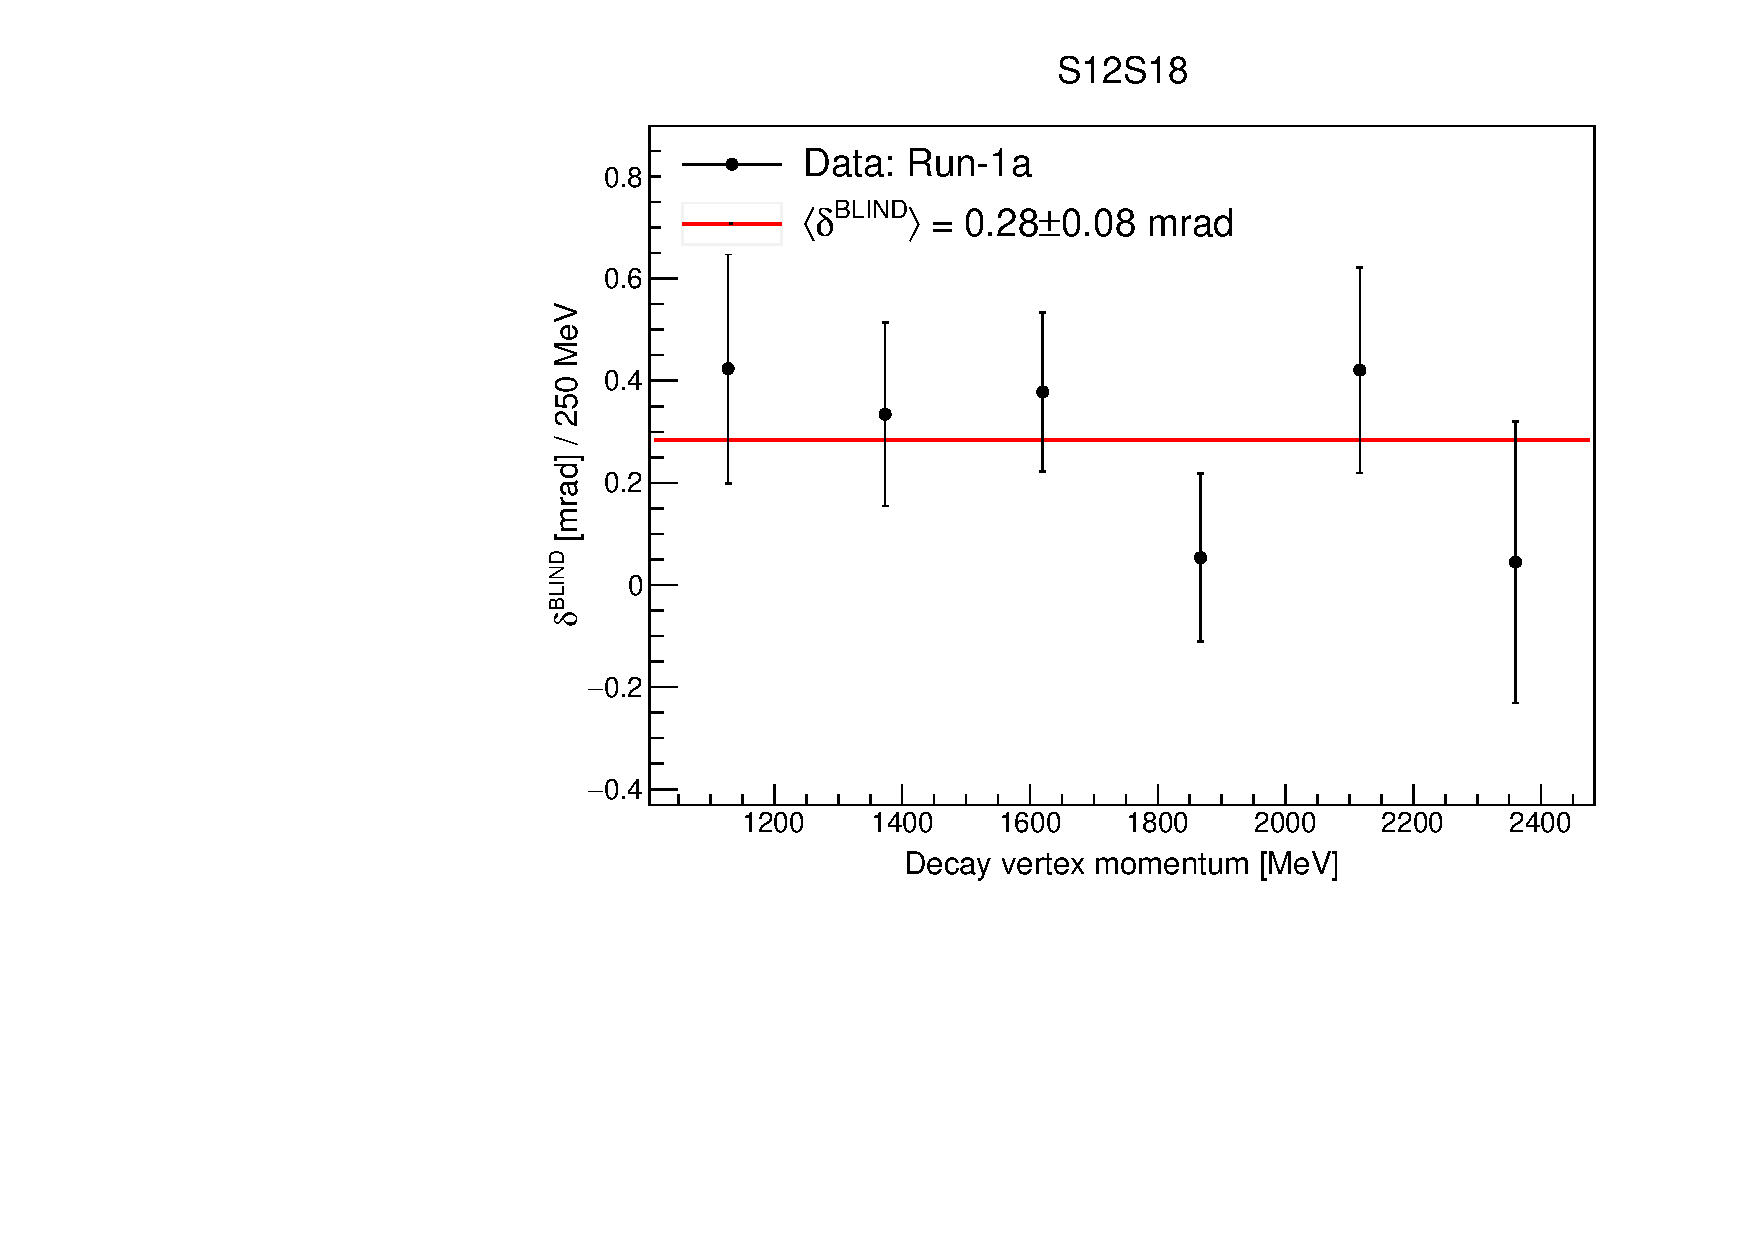
\includegraphics[trim={0 0 0 1cm},clip,width=.49\textwidth]{Images/Chapter6/S12S18_EDM_delta_prime_vs_p_1000-2500MeV_Run-1a_250MeV_1000_2500MeV_randomised_BQ.pdf}}
\subfloat[Run-1b.]{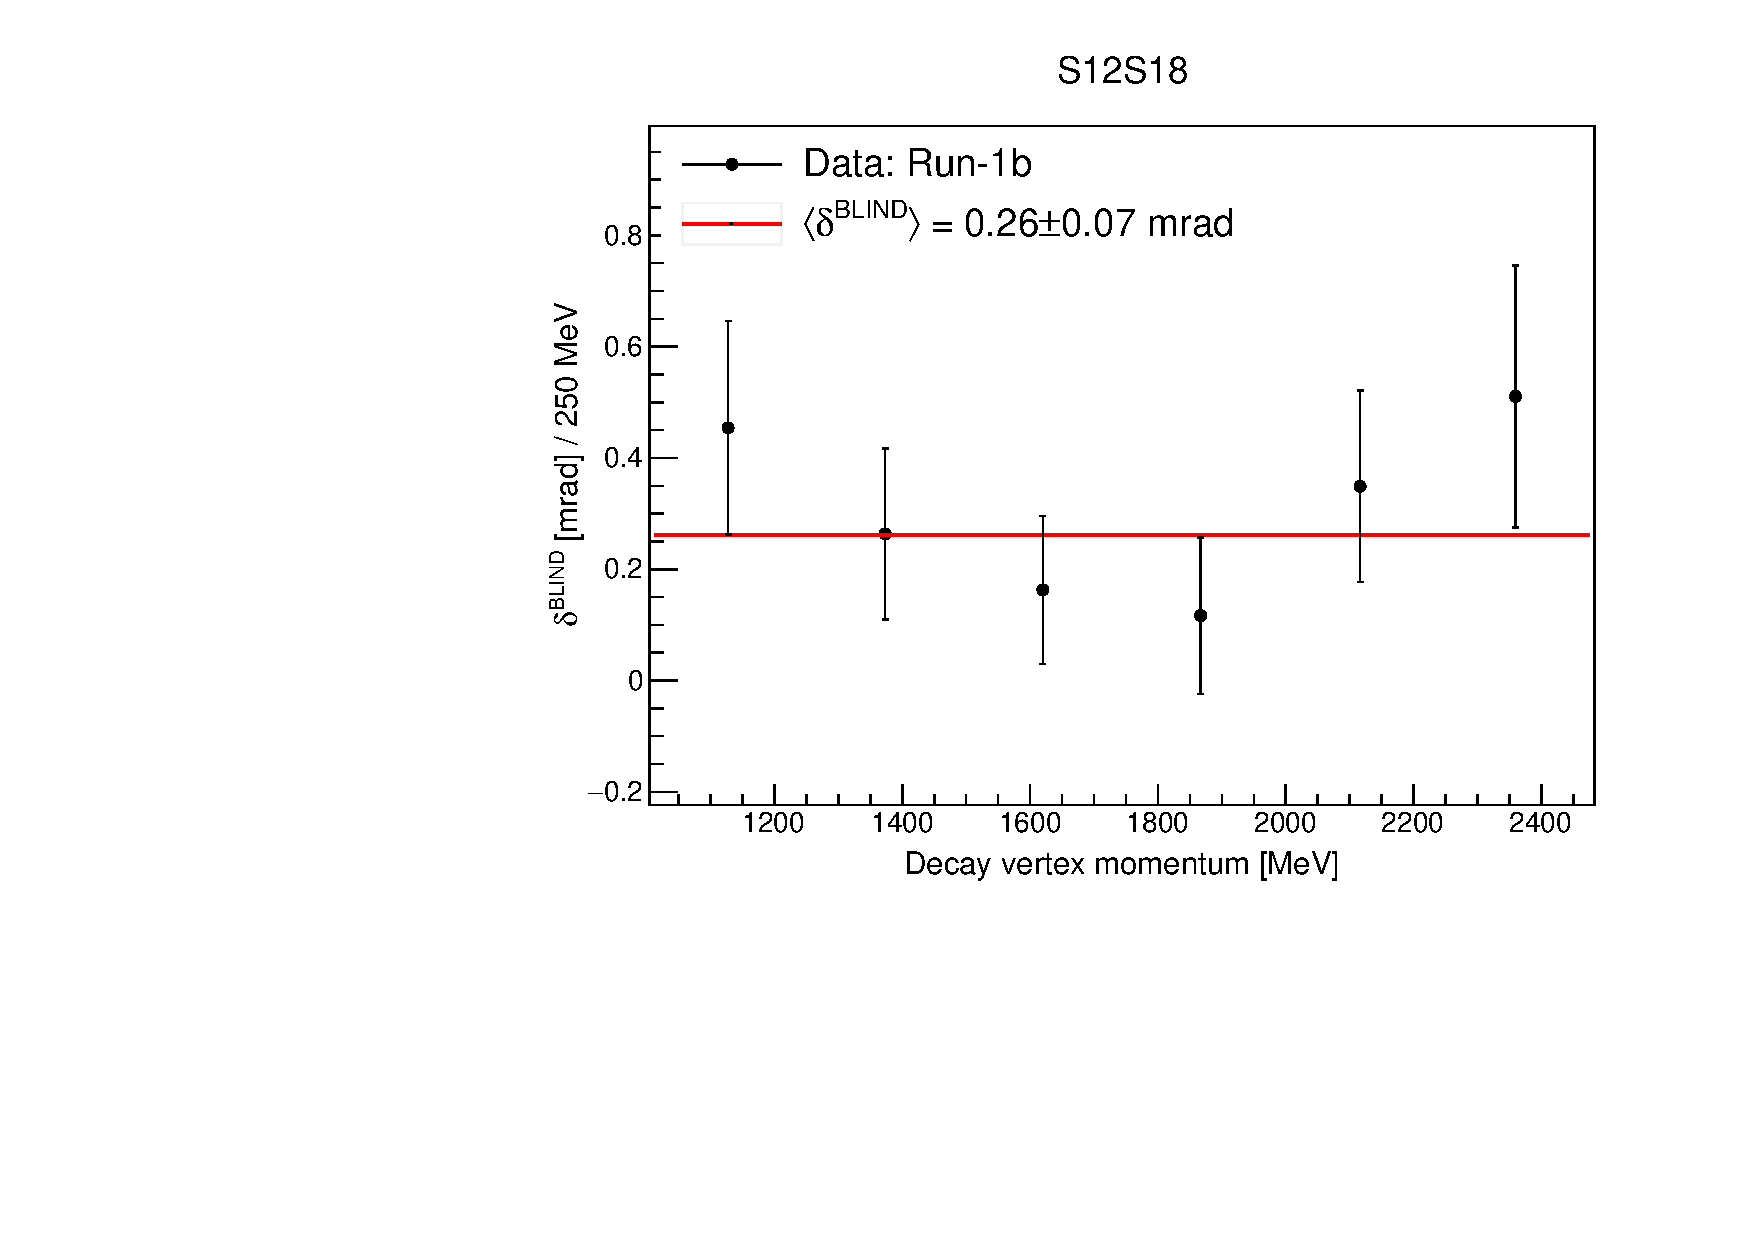
\includegraphics[trim={0 0 0 1cm},clip,width=.49\textwidth]{Images/Chapter6/S12S18_EDM_delta_prime_vs_p_1000-2500MeV_Run-1b_250MeV_1000_2500MeV_randomised_BQ.pdf}}\hfill
\subfloat[Run-1c.]{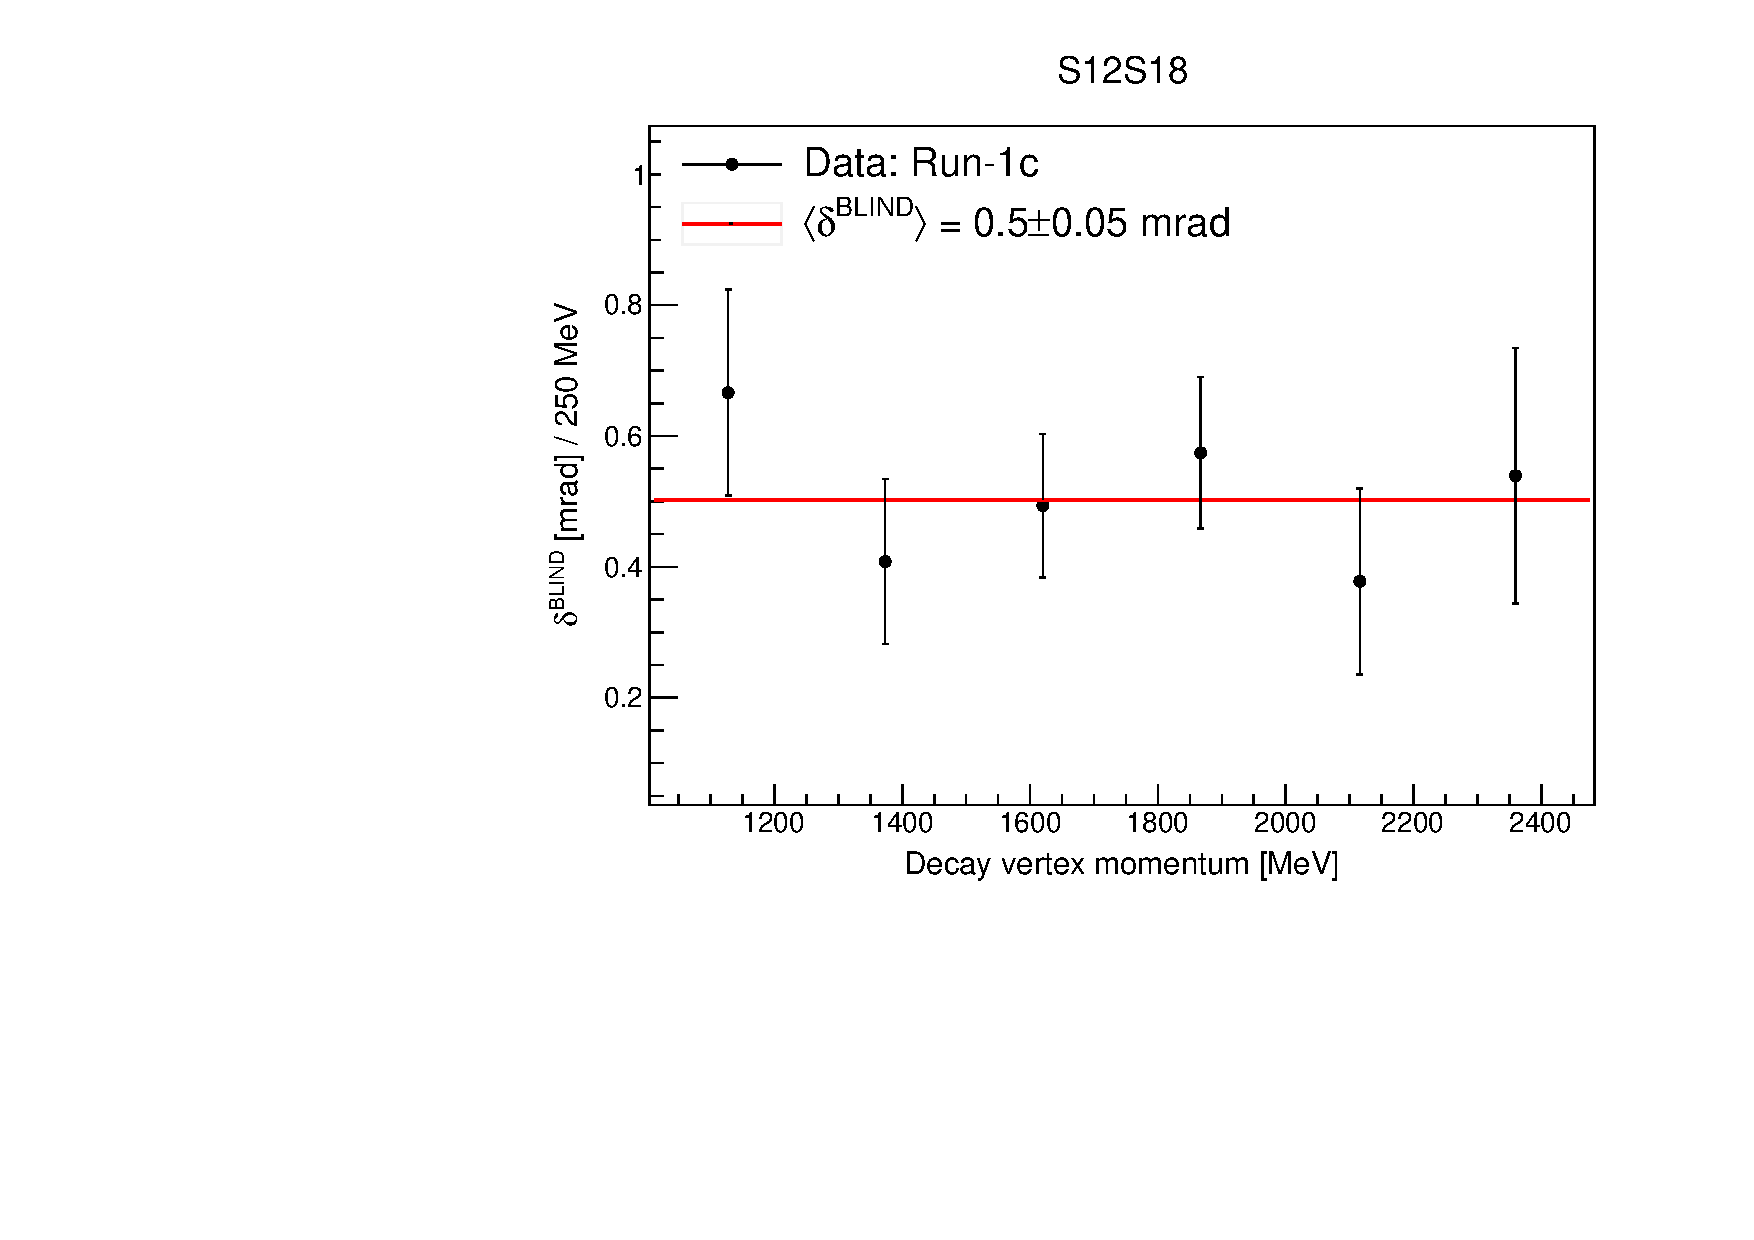
\includegraphics[trim={0 0 0 1cm},clip,width=.49\textwidth]{Images/Chapter6/S12S18_EDM_delta_prime_vs_p_1000-2500MeV_Run-1c_250MeV_1000_2500MeV_randomised_BQ.pdf}}
\subfloat[Run-1d.]{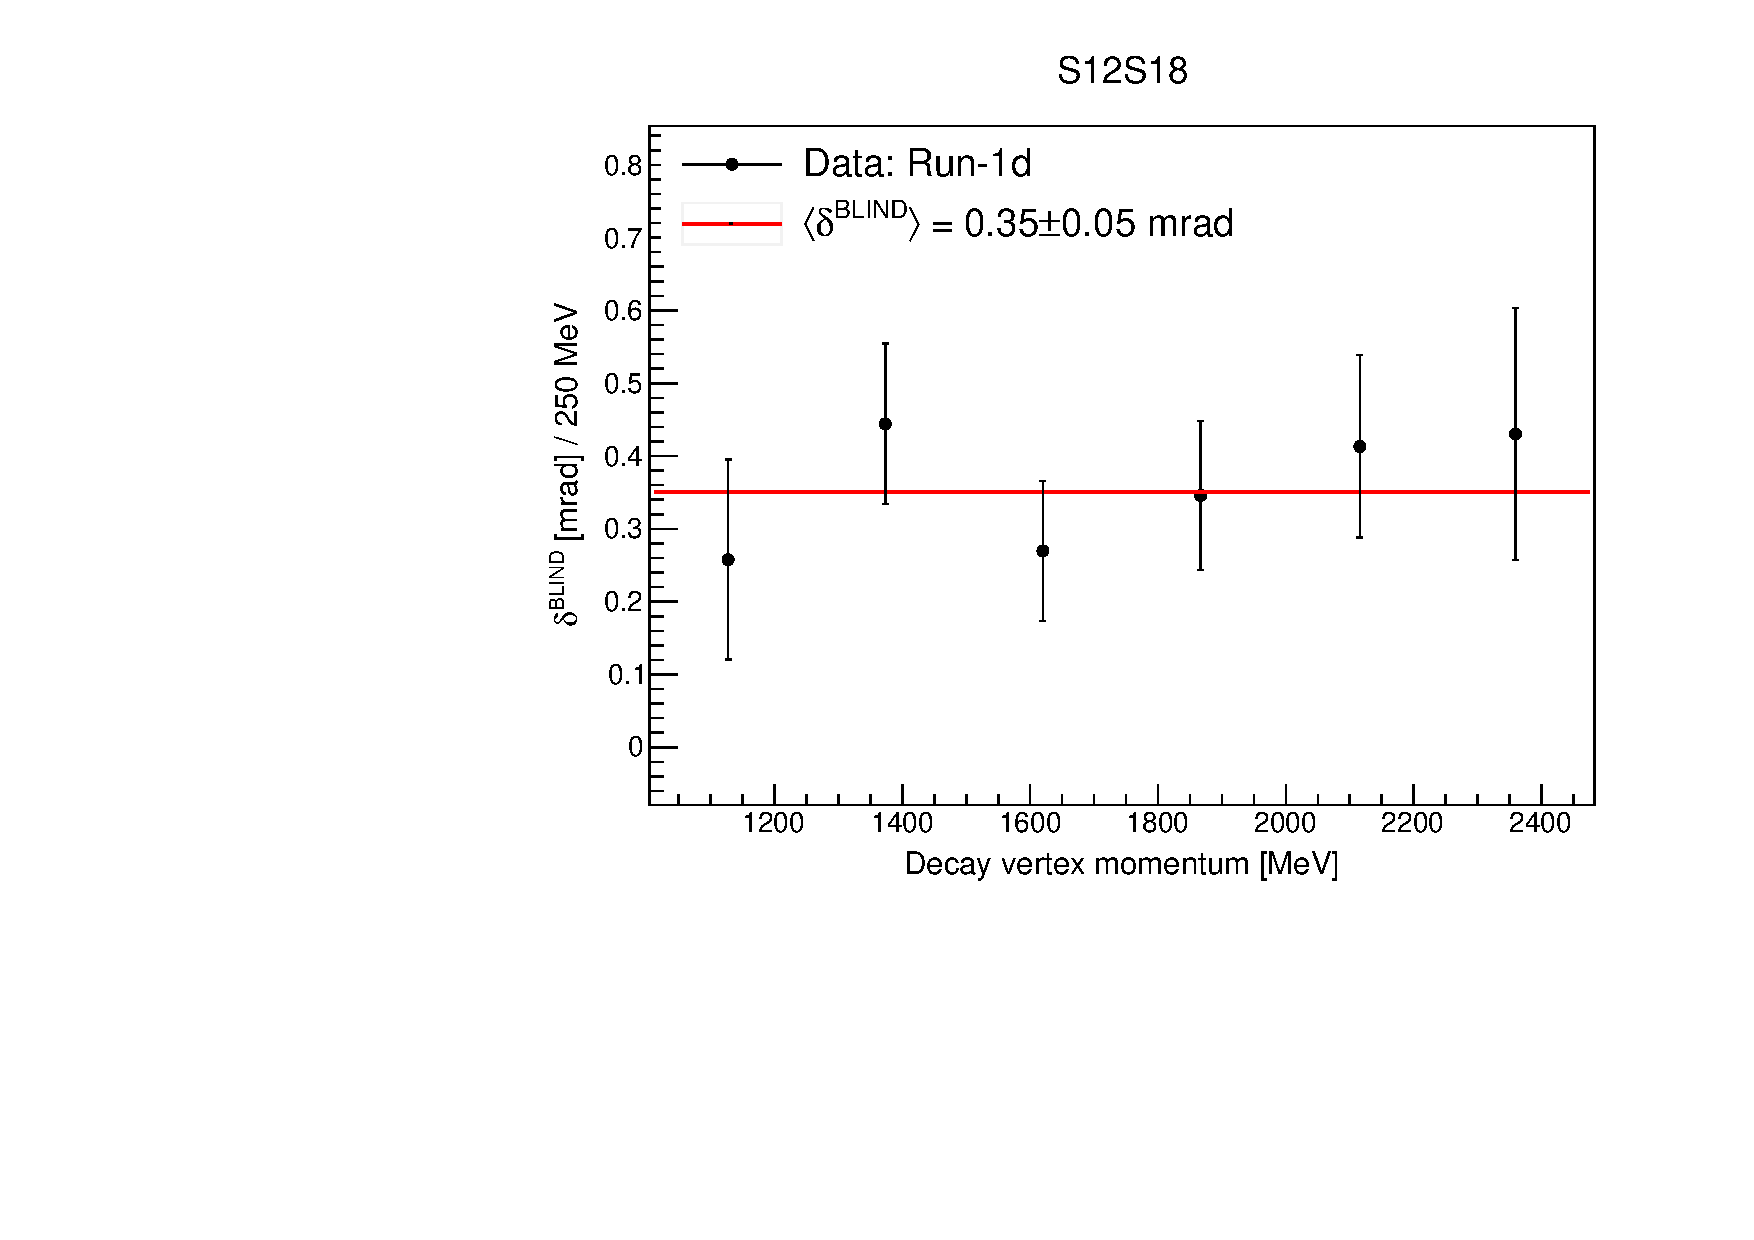
\includegraphics[trim={0 0 0 1cm},clip,width=.49\textwidth]{Images/Chapter6/S12S18_EDM_delta_prime_vs_p_1000-2500MeV_Run-1d_250MeV_1000_2500MeV_50usStartTime_randomised_BQ.pdf}}
\caption{$\delta^{\text{BLIND}}$ per momentum bin for each Run-1 dataset, with a zeroth order polynomial fit giving an uncertainty weighted average. Tracker stations 12 and 18 are combined.}
\label{fig:DeltaFits}
\end{figure}



% the product of the value obtained from evaluation of the dilution function, Equation \ref{eqn:Dilution}, at the average momentum of each bin and acceptance scale factor for that bin, presented in Figure \ref{fig:AcceptanceFactor}, is used as the total dilution correction factor. 

%where the product of the value obtained by evaluation of the dilution function, Equation \ref{eqn:DilutionFunction}, at the average momentum of that bin, and the $A_{\text{EDM}}$ acceptance scale factor, is taken as the total dilution correction factor. 

% In order to extract the laboratory frame tilt angle, $\delta$, from $A_{\text{EDM}}$ at a particular momentum interval, a correction must be applied which is specific to average momentum of that interval. In the case of 100\% acceptance (all decays), the correction factor may be found by simple evaluation of the dilution function, Equation \ref{eqn:DilutionFunction}. In the case where tracker acceptance is included (truth/reco vertices), the correction factor is the product of the value obtained from the dilution function and the appropriate $A_{\text{EDM}}$ acceptance factor. 


% value obtained from evaluation of Equation \ref{eqn:Dilution} at the mean momentum in each bin and acceptance scale factor for that bin, illustrated in Figure \ref{fig:AcceptanceFactor}, is used as the total dilution correction factor for $A_{\text{EDM}}$. 

The resulting distributions of $\delta^{\text{BLIND}}$ across momentum are fitted with a zeroth order polynomial for the uncertainty weighted average, $\langle \delta^{\text{BLIND}} \rangle$, which are shown in Figure \ref{fig:DeltaFits}, with tracker stations 12 and 18 combined. The measured average blinded tilt angles, $\langle\delta^{\text{BLIND}}\rangle$, are summarised in Table \ref{tbl:Run1MomBinnedTiltAngles}, where all uncertainties are statistical.% The uncertainties associated with the acceptance correction are discussed in Section \ref{sec:AcceptanceSyst}.

\begin{table}[t!]
\centering{}
\begin{tabular}{l|ccc}
\hline
\hline
\multirow{2}{*}{Dataset} & \multicolumn{3}{c}{$\langle\delta^{\text{BLIND}}\rangle$ [mrad]} \\ \cline{2-4}
& Station 12 & Station 18 & Combined \\ %& $d_{\mu}^{\text{BLIND}}$ [$\times10^{18}$ $e\cdot$cm] \\
\hline
Run-1a &  $0.42\pm0.10$ & $0.06\pm0.10$ & $0.28\pm0.08$\\
Run-1b &  $0.25\pm0.09$ & $0.25\pm0.10$ & $0.26\pm0.07$\\
Run-1c &  $0.51\pm0.07$ & $0.46\pm0.08$ & $0.50\pm0.05$\\ 
Run-1d &  $0.36\pm0.06$ & $0.34\pm0.07$ & $0.35\pm0.05$\\ 
\hline
\hline
\end{tabular}
\caption{Dilution corrected $\delta^{\text{BLIND}}$ results for the momentum-binned analysis.} 
\label{tbl:Run1MomBinnedTiltAngles}
\end{table}


\section{Systematic uncertainties, checks, and corrections}\label{sec:Run1Syst}


\subsection{The damaged ESQ resistors in Run-1}

Following the completion of data taking in Run-1, it was discovered that two out of the 32 resistors in the ESQ charging system had become damaged. As a consequence, the affected plates (Q1) possessed a slower RC (resistor-capacitor) time constant than designed \cite{OmegaARun1}\cite{BeamDynamics}. The resistors in question continued to deteriorate throughout Run-1, necessitating a delayed fit start-time in the Run-1d $\omega_{a}$ analysis of \SI{50}{\micro\second} (compared to \SI{30}{\micro\second}). The significance of this, in the context of the EDM search, is that the movement of the beam in the $x$-$y$ plane, which is normally associated with scraping, continues much later into the fill than intended: modifying the average accepted vertical angle. The damaged resistors and their repercussions are referenced again in the following sections. %The damaged resistors will be referenced multiple times in the following sections.

\subsection{Fit start-time scans}\label{sec:FitStartTimeScans}

The stability of the fit parameter $A_{\text{EDM}}^{\text{BLIND}}$ over a range of in-fill fit start-times is of particular interest in the context of the damaged resistors. To investigate this, fit start-time scans were performed using unmodulated fits over the range 1000-2500 MeV, where the minimum time of the fit was varied in units of $T_{g-2}$, from \SI{30.6}{\micro\second} to \SI{117.9}{\micro\second}. These scans are shown, with tracker stations 12 and 18 combined, for each Run-1 dataset in Figure \ref{fig:BasicFitStartTime}. The parabolic red bands indicate the allowed $1\sigma$ variation, $\sigma_{\Delta}$, between parameters measured from two datasets in the case where one is a subset of the other. This technique was developed specifically for the $\omega_{a}$ analysis at BNL \cite{BNLFinalReport}, where in this case the variation is given by
%
\begin{equation}
  \sigma_{\Delta} = \sqrt{\sigma_{2}^{2} - \sigma_{1}^{2}},
  \label{eqn:Kawall}
\end{equation}
%
where $\sigma_{2}$ is the uncertainty associated with the larger dataset (with an earlier fit start-time), and $\sigma_{1}$ indicates the uncertainty on the parameter measured using the sub-dataset. 

In all cases, the majority of data points fall within the allowed deviation. However, in the case of Run-1d, the rapid decrease in $A_{\text{EDM}}^{\text{BLIND}}$ prior to \SI{50}{\micro\second} was taken as an indication that a later fit start-time should be used (\SI{52.3}{\micro\second} or $12\times T_{g-2}$), since this variation is likely a consequence of the deteriorating ESQ resistors. 

\begin{figure}[t!]
\centering{}
\subfloat[Run-1a.]{\includegraphics[trim={0 0 0 .9cm},clip,width=.49\textwidth]{Images/Chapter6/FitStartTime_Run-1a.pdf}}
\subfloat[Run-1b.]{\includegraphics[trim={0 0 0 .9cm},clip,width=.49\textwidth]{Images/Chapter6/FitStartTime_Run-1b.pdf}}\hfill

\subfloat[Run-1c.]{\includegraphics[trim={0 0 0 .9cm},clip,width=.49\textwidth]{Images/Chapter6/FitStartTime_Run-1c.pdf}}
\subfloat[Run-1d.]{\includegraphics[trim={0 0 0 .9cm},clip,width=.49\textwidth]{Images/Chapter6/FitStartTime_Run-1d.pdf}}
\caption{Fit start-time scans for unmodulated vertical angle fits over the range 1000-2500 MeV. As discussed in the text, the parabolic red bands indicate the allowed $1\sigma$ variation according to the changing statistical uncertainty across the scan. The deviation shown in Run-1d prior to \SI{50}{\micro\second} was taken as an indication that a delayed fit start-time should be used for this dataset.}
\label{fig:BasicFitStartTime}
\end{figure} 

\subsection{The time and momentum dependence of the average vertical angle}\label{subsec:AvgVertAngleData}
% As introduced in Chapter \ref{chap:5} Section \ref{sec:AvgVertAngleSim}, the average vertical angle, $\langle \theta_{y} \rangle$, demonstrates a momentum dependence
As introduced in Chapter \ref{chap:5} Section \ref{sec:AvgVertAngleSim}, the average vertical angle, $\langle \theta_{y} \rangle$, demonstrates a momentum dependence in simulation, which is attributed to tracker acceptance effects in Section \ref{sec:AcceptanceWeightings} of that chapter. This dependence is also present in Run-1 data, as illustrated in Figure \ref{fig:AvgVertAngleDataAndSim}, which also highlights the difference between the distributions of $\langle \theta_{y} \rangle(p)$ measured in Run-1 and those measured in simulation, as well as the variation between Run-1 datasets. The Run-1 datasets generally exhibit a more prominent average offset than simulation at low momentum, which is most pronounced in Run-1d. This likely indicates a contribution from damaged ESQ resistors, where the increased vertical movement of the beam, and changing vertical angle acceptance, would provide a logical explanation for the observed behaviour. At present, no adjustment to the acceptance correction is made to account for this difference, although a correction will be made before the results are unblinded.

\begin{figure}[h!]
\centering{}
\includegraphics[trim={0 0 0 0cm},clip,width=.69\textwidth]{Images/Chapter6/verticalOffsetIllustration_noVertCorr.pdf}
\caption{The momentum dependence of the average vertical angle, comparing the results from the simulation, discussed in Chapter \ref{chap:5}, and the Run-1 datasets.}
\label{fig:AvgVertAngleDataAndSim}
\end{figure} 

As a further consequence of the damaged ESQ resistors, $\langle \theta_{y} \rangle$ also acquires an in-fill time dependence, which, again, is most pronounced in Run-1d. This time dependence is parametrised by fitting $\langle \theta_{y} \rangle$, binned at the cyclotron period, with a fit function consisting of two exponential terms and a constant offset, $c$, as follows:
%
\begin{equation}
  \langle \theta_{y} \rangle (t) = \frac{A}{\tau_{A}}e^{\frac{-t}{\tau_{A}}}+\frac{B}{\tau_{B}}e^{\frac{-t}{\tau_{B}}} + c.
  \label{eqn:DoubleExponential}
\end{equation}
% 
The first term relates to the slow change in the electric field due to the damaged resistors, with an amplitude $A$ and time constant $\tau_{A}$. The second term contains an amplitude $B$ and faster time constant, $\tau_{B}$, which relates to the $\sim7$ \SI{}{\micro\second} scraping period. Tracker stations are treated independently, with fits to station 12 data over the 1000-2500 MeV momentum range shown in Figure \ref{fig:S12TimeDependenceCorr}. The time constants are fixed to the values reported by J. Mott during the Run-1 $\omega_{a}$ analysis \cite{MottTimeConstants}. These fits are performed in momentum bins in order to perform a simultaneous correction of the momentum-dependent offset, using the parameter $c$ as a proxy for $\langle \theta_{y} \rangle$, and the time-dependent variation by evaluation of the fit function at the positron decay time. 

\begin{figure}[t!]
\centering{}
\subfloat[Run-1a.]{\includegraphics[trim={0 0 0 .9cm},clip,width=.49\textwidth]{Images/Chapter6/S12_ThetaYvsTimeFit_Run-1a_BQ.pdf}}
\subfloat[Run-1b.]{\includegraphics[trim={0 0 0 .9cm},clip,width=.49\textwidth]{Images/Chapter6/S12_ThetaYvsTimeFit_Run-1b_BQ.pdf}}\hfill
\subfloat[Run-1c.]{\includegraphics[trim={0 0 0 .9cm},clip,width=.49\textwidth]{Images/Chapter6/S12_ThetaYvsTimeFit_Run-1c_BQ.pdf}}
\subfloat[Run-1d.]{\includegraphics[trim={0 0 0 .9cm},clip,width=.49\textwidth]{Images/Chapter6/S12_ThetaYvsTimeFit_Run-1d_BQ.pdf}}
\caption{Double exponential fits to the in-fill time dependence of $\langle \theta_{y} \rangle$, for tracker station 12. This phenomenon is unique to Run-1, and is attributed to non-typical beam movement due caused by the two damaged ESQ resistors. The time constants, $\tau_{A}$ and $\tau_{B}$, are fixed to the values reported by J. Mott in the Run-1 $\omega_{a}$ analysis \cite{MottTimeConstants}.}
\label{fig:S12TimeDependenceCorr}
\end{figure} 

\begin{table}[t!]
\centering{}
\begin{tabular}{l|ccccc}
\hline
\hline
 & Run-1a & Run-1b & Run-1c & Run-1d & Avg. \\ 
 \hline
$\Delta \langle \delta^{\text{BLIND}} \rangle $ [mrad] & $-0.00996$ & $-0.00862$ & $-0.00679$ & $-0.0148$ & $-0.0100$ \\ 
% $\Delta \sigma_{\delta^{\text{BLIND}}}$ [mrad] & $-1.00\times10^{-6}$ & $0.00$ & $-0.00679$ & $-0.0100$ \\ 
\hline
\hline
\end{tabular}
\caption{The change in $\langle \delta^{\text{BLIND}} \rangle$ following the $\langle \theta_{y} \rangle$ offset correction.}
\label{tbl:VertOffDiff}
\end{table}

The impact of this correction is given in terms of the change in $\langle \delta^{\text{BLIND}} \rangle$, summarised for each dataset in Table \ref{tbl:VertOffDiff}, showing a small reduction with an average value in Run-1 of \SI{10}{\micro\radian}. No change is observed in the average fit $\chi^{2}/\text{NDF}$, and the change in the uncertainty on $\langle \delta^{\text{BLIND}} \rangle$ is $\mathcal{O}(10^{-6})$ mrad, which is negligible. 

%which is a factor of $\sim10$ less than $\tau_{A}$ 
% Since this momentum dependence is an acceptance related phenomenon, it may be argued that the observed difference between simulation and data arise from a difference between the relative position of the beam to the trackers in Run-1 compared with simulation. This might be due to the closed orbit distortion, or 

%  to time dependent average vertical decay angle, which . . Station 12. }



\subsection{Beam dynamics corrections}\label{subsec:BeamDynamicsCorr}
 
The muon beam does not propagate in a perfect static orbit. Beam dynamics effects, betatron oscillations in particular (introduced in Chapter \ref{chap:2} Section \ref{sec:BeamDynamics}) modify the average position of the beam as a function of time; resulting in an oscillating average vertical angle at the relevant betatron frequency. Although the modulation of decay times at $T_{g-2}$, discussed in Chapter \ref{chap:5} Section \ref{sec:TimeMod}, is designed to de-phase and therefore minimise oscillations such as this, their potential impact must be investigated nonetheless.

\begin{figure}[b!]
\centering{}
\subfloat[Run-1a.]{\includegraphics[trim={0 0 0 0},clip,width=.49\textwidth]{Images/Chapter6/S12S18_FFT_noRand_Run-1a.pdf}}
\subfloat[Run-1b.]{\includegraphics[trim={0 0 0 0},clip,width=.49\textwidth]{Images/Chapter6/S12S18_FFT_noRand_Run-1b.pdf}}\hfill
\subfloat[Run-1c.]{\includegraphics[trim={0 0 0 0},clip,width=.49\textwidth]{Images/Chapter6/S12S18_FFT_noRand_Run-1c.pdf}}
\subfloat[Run-1d.]{\includegraphics[trim={0 0 0 0},clip,width=.49\textwidth]{Images/Chapter6/S12S18_FFT_noRand_Run-1d.pdf}}
\caption{FFTs of the residual distributions from unmodulated vertical angle oscillation fits, from \SI{30.6}{\micro\second} onwards, showing no obvious peaks in the frequency domain.}
\label{fig:AllTimeFFTsNoRand}
\end{figure}

\begin{figure}[t!]
\centering{}
\subfloat[Run-1a.]{\includegraphics[trim={0 0 0 0},clip,width=.49\textwidth]{Images/Chapter6/S12S18_FFT_earlyTimes_overlay_Run-1a.pdf}}
\subfloat[Run-1b.]{\includegraphics[trim={0 0 0 0},clip,width=.49\textwidth]{Images/Chapter6/S12S18_FFT_earlyTimes_overlay_Run-1b.pdf}}\hfill
\subfloat[Run-1c.]{\includegraphics[trim={0 0 0 0},clip,width=.49\textwidth]{Images/Chapter6/S12S18_FFT_earlyTimes_overlay_Run-1c.pdf}}
\subfloat[Run-1d.]{\includegraphics[trim={0 0 0 0},clip,width=.49\textwidth]{Images/Chapter6/S12S18_FFT_earlyTimes_overlay_Run-1d.pdf}}
\caption{FFTs of the residual distributions from unmodulated vertical angle oscillation fits over a time range of 30.6-65.5 \SI{}{\micro\second}. The uncorrected black distributions show prominent peaks at the vertical betatron frequency, $f_{y}$, in all datasets except Run-1d, where it is significantly reduced. A small peak at the aliased horizontal betatron frequency, $f_{CBOx}$, is also visible in Run-1d. Uniform randomisation of decay times about $\pm T_{f_{y}}/2$ removes the vertical betatron oscillation peak, as shown by the corrected distributions in red.}
\label{fig:EarlyTimeFFTsOverlay}
\end{figure}

To assess the presence of additional oscillations in data, fast Fourier transforms (FFTs) were performed on the residual distributions from fits to the unmodulated vertical angle oscillation, binned in time at the cyclotron period. Modulated fits were not used in this case because the relatively low number of time bins results in poor resolution in the frequency domain. Fit residual FFTs are shown for each Run-1 dataset for all times after \SI{30.6}{\micro\second} in Figure \ref{fig:AllTimeFFTsNoRand}, showing no clear peaks. However, the betatron oscillation amplitude decays exponentially with time, so FFTs were performed over earlier time range in-fill, 30.6-65.5 \SI{}{\micro\second}, where betatron motion is more prominent. These early-time FFTs are given by the black distributions in Figure \ref{fig:EarlyTimeFFTsOverlay}, showing prominent peaks at the vertical betatron frequency, $f_{y}$, in all datasets with the exception of Run-1d, where it is greatly reduced. Additionally, the FFTs for Run-1d possess a small peak at the aliased horizontal betatron frequency, $f_{CBOx}$. The frequencies $f_{y}$ and $f_{CBOx}$ are listed in Table \ref{tbl:Frequencies}. To remove the vertical betatron oscillation, decay times were randomly drawn from a uniform distribution $\pm T_{f_{y}}/2$ about the measured time, where fit residual FFTs for the time randomised datasets are shown in red in Figure \ref{fig:EarlyTimeFFTsOverlay}, with no peaks at $f_{y}$. Removal of the horizontal betatron oscillation in this way is not possible due to its much longer time period, where randomisation would obfuscate a potential EDM oscillation. Since the $f_{CBOx}$ peak is relatively small, as well as only being present in Run-1d -- which also utilises a delayed fit start-time -- no attempt to remove the horizontal betatron oscillation was made in this analysis. As a precaution, the fast rotation frequency was also removed using the time randomisation technique, in addition to binning at the cyclotron period. 

The impact of time randomisation is assessed according to the change in $\langle \delta^{\text{BLIND}} \rangle$, where the values measured with time randomisation are subtracted from those measured without it. The change in the uncertainty, $\sigma_{\langle \delta^{\text{BLIND}} \rangle}$, and the average fit $\chi^{2}/\text{NDF}$ across momentum bins, are also considered. As is summarised in Table \ref{tbl:RandDeltaDiff}: the fit $\chi^{2}/\text{NDF}$ is, on average, significantly reduced with the inclusion of time randomisation; the average $\langle \delta^{\text{BLIND}} \rangle$ decreases by $-0.0437$ mrad; and the uncertainty is largely unaffected, increasing by \SI{4.85}{\micro\radian}, which is an order of magnitude less than the statistical uncertainty associated the largest dataset (Run-1d). The delayed fit start-time in Run-1d means that the impact on the results from this dataset is negligible. 

\begin{table}[t!]
\centering{}
\begin{tabular}{l|ccccc}
\hline
\hline
 & Run-1a & Run-1b & Run-1c & Run-1d & Avg. \\ 
 \hline
$\Delta \chi^{2}/\text{NDF}$ & $-0.243$ & $-0.32$ & $-0.40$ & $0.00$ & $-0.243$ \\
$\Delta \langle \delta^{\text{BLIND}} \rangle$ [mrad] & $-0.0736$ & $-0.118$ & $0.0166$ & $4.3\times10^{-5}$ & $-0.0437$ \\
$\Delta \sigma_{\langle \delta^{\text{BLIND}} \rangle}$ [mrad] & $-0.00389$ & $0.0126$ & $0.0107$ & $-1.0\times10^{-6}$ & $0.00485$ \\
\hline
\hline
\end{tabular}
\caption{The impact of time randomisation on $\langle \delta^{\text{BLIND}} \rangle$, summarising the changes in: the average fit $\chi^{2}/\text{NDF}$, the central value, and the uncertainty.} 
\label{tbl:RandDeltaDiff}
\end{table}

\subsection{Phase uncertainty assessment}\label{sec:PhaseUnc}

% The analysis described in Chapter \ref{chap:6} depends on an accurate measurement of the anomalous precession oscillation phase, $\phi$, which is shown in Figure \ref{fig:Run1Phases}. 

The anomalous precession oscillation phase, $\phi$ is a fixed parameter in the EDM analysis, despite possessing an uncertainty, $\sigma_{\phi}$. To evaluate the potential effect of this uncertainty on $\langle \delta^{\text{BLIND}} \rangle$, $\phi$ was fixed to a value $\pm \sigma_{\phi}$ and propagated through the analysis. The change in $\langle \delta^{\text{BLIND}} \rangle$ for both signs was found to be of the sub-\SI{}{\micro\radian} level, as shown in Table \ref{tbl:Run1PhaseUncertainty}, and is therefore negligible.

\clearpage 

\begin{table}[h!]
\centering{}
\begin{tabular}{l|ccc}
\hline
\hline
\multirow{2}{*}{Dataset} & \multirow{2}{*}{$\sigma_{\phi}$ [mrad]} & \multicolumn{2}{c}{$\Delta \langle \delta^{\text{BLIND}} \rangle$ [\SI{}{\micro\radian}]} \\ 
& & $\phi+\sigma_{\phi}$ &  $\phi-\sigma_{\phi}$ \\
\hline
Run-1a & $3.62$ & $0.187$ & $-0.132$ \\ 
Run-1b & $3.05$ & $0.183$ & $-0.393$ \\ 
Run-1c & $2.55$ & $0.117$ & $-0.0740$ \\ 
Run-1d & $2.21$ & $0.0180$ & $-0.0180$ \\ 
\hline
\hline
\end{tabular}
\caption{The change in $\langle \delta^{\text{BLIND}} \rangle$ with the measured anomalous precession oscillation phase, $\phi$, shifted by $\pm\sigma_{\phi}$.} 
\label{tbl:Run1PhaseUncertainty}
\end{table}

\subsection{Tracker vertical angle resolution}\label{subsec:TrackResolution}

A further potential source of systematic uncertainty is the trackers' ability to resolve the average vertical angle, $\langle \theta_{y} \rangle$. To quantify this, the same simulation dataset as was employed in the tracker acceptance study, detailed in Chapter \ref{chap:5}, was used to produce distributions of the true vertical angle subtracted from the measured (reco) vertical angle. The true and reco distributions of $\theta_{y}$ are shown in Figures \ref{subfig:TrueThetaY} and \ref{subfig:RecoThetaY}, and the distribution of the differences is shown in Figure \ref{subfig:VerticalAngleResolution}. Only tracks with momentum in the range of 1000-2500 MeV were used. The average vertical angle resolution is equal to the uncertainty on the mean, which is
%
\begin{align*}
    \delta \langle \Delta \theta_{y} \rangle = \, \text{\SI{3}{\micro\radian}}. 
    % \text{\SI{3}{\micro\radian}}. \\
\end{align*}
%
Given that the uncertainty on the mean for both true and measured $\theta_{y}$ distributions, formed from the same simulated dataset, is one order of magnitude larger than this, the contribution from tracker resolution to the uncertainty on $A_{\text{EDM}}$, and by extension $\langle \delta^{\text{BLIND}} \rangle$, can be assumed to be negligible. As an additional point, the distribution of $\delta \langle \Delta \theta_{y} \rangle$ per 100 MeV momentum bin is shown in Figure \ref{subfig:VerticalAngleResolutionScan}: where the optimum resolution is obtained in the range 1000-2500 MeV, which is the same as is used in the analysis presented in this chapter.

\begin{figure}[t!]
\centering{}
\subfloat[]{\includegraphics[trim={0 0 0 0},clip,width=.49\textwidth]{Images/Chapter6/theta_y_true.pdf}\label{subfig:TrueThetaY}}
\subfloat[]{\includegraphics[trim={0 0 0 0},clip,width=.49\textwidth]{Images/Chapter6/theta_y_reco.pdf}\label{subfig:RecoThetaY}}\hfill

\subfloat[]{\includegraphics[trim={0 0 0 0},clip,width=.49\textwidth]{Images/Chapter6/theta_y_res.pdf}\label{subfig:VerticalAngleResolution}}
\subfloat[]{\includegraphics[trim={0 0 0 0},clip,width=.49\textwidth]{Images/Chapter6/theta_y_avg_res_vs_p.pdf}\label{subfig:VerticalAngleResolutionScan}}
\caption{The straw tracker vertical angle resolution, showing: (a) the $\theta_{y}$ distribution for measured (reco) track decay vertices; (b) the $\theta_{y}$ distribution for truth decay vertices; (c) the distribution of truth minus measured $\theta_{y}$, where the $\langle \theta_{y} \rangle$ resolution is given by the error on the mean; (d) $\langle \theta_{y} \rangle$ resolution in 100 MeV momentum intervals.}
\label{fig:VerticalAngleResolutionPlots}
\end{figure} 

\subsection{Tracker acceptance}\label{sec:AcceptanceSyst}

The correction required to scale the measured $A_{\text{EDM}}^{\text{BLIND}}$ to $\delta^{\text{BLIND}}$, discussed in Section \ref{sec:ExtractTiltData}, relies on an acceptance correction with an associated statistical uncertainty from Monte Carlo, and a systematic uncertainty associated with tracker global alignment. The procedure for assessing these uncertainties follows the method detailed in Chapter \ref{chap:5} Sections \ref{sec:AcceptDilFactor} and \ref{sec:Alignment}. 

\begin{figure}[t!]
\centering{}
\subfloat[Run-1a.]{\includegraphics[trim={0 0 0 0.9cm},clip,width=.49\textwidth]{Images/Chapter6/S12S18_EDM_delta_prime_hist_1000_1000-2500MeV_Run-1a_250MeV_1000_2500MeV_randomised_BQ.pdf}}
\subfloat[Run-1b.]{\includegraphics[trim={0 0 0 0.9cm},clip,width=.49\textwidth]{Images/Chapter6/S12S18_EDM_delta_prime_hist_1000_1000-2500MeV_Run-1b_250MeV_1000_2500MeV_randomised_BQ.pdf}}\hfill
\subfloat[Run-1c.]{\includegraphics[trim={0 0 0 0.9cm},clip,width=.49\textwidth]{Images/Chapter6/S12S18_EDM_delta_prime_hist_1000_1000-2500MeV_Run-1c_250MeV_1000_2500MeV_randomised_BQ.pdf}}
\subfloat[Run-1d.]{\includegraphics[trim={0 0 0 0.9cm},clip,width=.49\textwidth]{Images/Chapter6/S12S18_EDM_delta_prime_hist_1000_1000-2500MeV_Run-1d_250MeV_1000_2500MeV_50usStartTime_randomised_BQ.pdf}}
\caption{The distributions of $\langle \delta^{\text{BLIND}} \rangle$, populated via 1000 trials where the acceptance dilution factor per momentum bin was randomly drawn from a Gaussian distribution with a mean equal to the acceptance factor and a width equal to its statistical uncertainty. The width of these distributions was taken as the contribution to the uncertainty on $\delta^{\text{BLIND}}$ arising from the statistical uncertainty associated with the simulation dataset used to determine said acceptance factors.}
\label{fig:AcceptanceStatErrorData}
\end{figure} 

In the same manner as illustrated in Figure \ref{fig:AcceptanceStatError}, the acceptance statistical uncertainty from simulation was taken as the width of a distribution of $\langle \delta^{\text{BLIND}} \rangle$ results, populated via 1000 trials where the acceptance dilution factor per momentum bin was randomly drawn from a Gaussian distribution with a mean equal to the acceptance factor and a width equal to its statistical uncertainty. These distributions are shown in Figure \ref{fig:AcceptanceStatErrorData} for each Run-1 dataset. The corresponding uncertainties are tabulated, along with the alignment uncertainties, in Table \ref{tbl:MainResultUnc}, and are included in the total uncertainty on the final result.

\subsection{The radial magnetic field}

The uncertainties associated with the radial magnetic field per Run-1 dataset are discussed at length in Chapter \ref{chap:4} and summarised in Table \ref{tbl:BrResults}. These uncertainties are reproduced in units of mrad and $e\cdot$cm in Table \ref{tbl:MainResultUnc}, presenting a small contribution to the total uncertainty. 

\begin{landscape}

\subsection{Table of uncertainties}

\thispagestyle{empty}
% A preliminary table of all uncertainties contributing to the main result, shown in Figure \ref{fig:MainResult}.

A full summarisation of all uncertainties contributing to the final result is given in Table \ref{tbl:MainResultUnc}, where the dominant uncertainties are statistical. The uncertainties associated with tracker acceptance and alignment preliminary. %are are expected to decrease as the size of the Monte Carlo datasets used to to derive them increases, and the uncertainties associated with tracker alignment are preliminary, as discussed in Chapter \ref{chap:5} Section \ref{sec:Alignment}.

\begin{table}[h!]
\centering{}
\begin{tabular}{ll|cc|cc|cc|cc}
\cline{3-10}
\cline{3-10}
 % & \multirow{2}{*}{$\delta^{\text{BLIND}}$ [mrad]} & \multicolumn{2}{c}{$\d_{\mu}^{\text{BLIND}}$ $e\cdot$cm  \\ 
& & \multicolumn{2}{c|}{Run-1a} & \multicolumn{2}{c|}{Run-1b} & \multicolumn{2}{c|}{Run-1c} & \multicolumn{2}{c}{Run-1d} \\ \cline{3-10}
&  & $\delta$ [mrad] & $d_{\mu}$ [$\times10^{-19}$ $e\cdot$cm] & $\delta$ [mrad] & $d_{\mu}$ [$\times10^{-19}$ $e\cdot$cm] & $\delta$ [mrad] & $d_{\mu}$ [$\times10^{-19}$ $e\cdot$cm] & $\delta$ [mrad] & $d_{\mu}$ [$\times10^{-19}$ $e\cdot$cm] \\\cline{3-10}   
% \\
\cline{2-10}  
\hspace{-6em}\ldelim\{{5}{*}[Station 12] 
& Statistical  & 0.0996 & 3.18 & 0.0851 & 2.72 & 0.0698 & 2.23 & 0.0613 & 1.96 \\
& Acceptance     & 0.0292 & 0.931 & 0.0159 & 0.507 & 0.0322 & 1.03 & 0.0223 & 0.712 \\
& Alignment     & 0.0240 & 0.768 & 0.0120 & 0.382 & 0.0274 & 0.874 & 0.0182 & 0.580 \\
& Radial magnetic field  & 0.00730 & 0.233 & 0.00817 & 0.261 & 0.00824 & 0.263 & 0.00915 & 0.292 \\
\cdashline{2-10}
& Total         & 0.107 & 3.41 & 0.0878 & 2.80 & 0.0820 & 2.62 & 0.0683 & 2.18 \\  
\cline{2-10}
\hspace{-6em}\ldelim\{{5}{*}[Station 18] 
& Statistical   & 0.120 & 3.83 & 0.102 & 3.27 & 0.0849 & 2.71 & 0.0745 & 2.38 \\
& Acceptance    & 0.0220 & 0.701 & 0.0236 & 0.753 & 0.0343 & 1.10 & 0.0270 & 0.863 \\
& Alignment     & 0.00654 & 0.209 & 0.000792 & 0.0253 & 0.0140 & 0.445 & 0.0218 & 0.697 \\
& Radial magnetic field  & 0.00730 & 0.233 & 0.00817 & 0.261 & 0.00824 & 0.263 & 0.00915 & 0.292 \\
\cdashline{2-10}
& Total         & 0.122 & 3.90 & 0.105 & 3.37 & 0.0930 & 2.97 & 0.0827 & 2.64 \\ 
\cline{2-10} 
% \multirow{4}{*}{Station 12} 
\hspace{-6em}\ldelim\{{5}{*}[Combined] 
& Statistical & 0.0774 & 2.47 & 0.0662 & 2.11 & 0.0545 & 1.74 & 0.0479 & 1.53 \\
& Acceptance & 0.0151 & 0.481 & 0.0138 & 0.440 & 0.0241 & 0.769 & 0.0164 & 0.524 \\
& Alignment & 0.0137 & 0.436 & 0.00762 & 0.243 & 0.02351 & 0.750 & 0.0203 & 0.649 \\
& Radial magnetic field & 0.00730 & 0.233 & 0.00817 & 0.261 & 0.00824 & 0.263 & 0.00915 & 0.292 \\
\cdashline{2-10}
& Total & 0.0804 & 2.57 & 0.0685 & 2.19 & 0.0646 & 2.06 & 0.0553 & 1.76 \\
\cline{2-10}
\cline{2-10}
\end{tabular}
\caption{A preliminary table of uncertainties contributing to the main result, shown in Figure \ref{fig:MainResult}.}
\label{tbl:MainResultUnc}
\end{table}

\end{landscape}

\section{Results}\label{sec:EDMResults}

Finally, the contribution to the precession plane tilt angle from the radial magnetic field was subtracted from the $\langle \delta^{\text{BLIND}} \rangle$ results, summarised in Table \ref{tbl:Run1MomBinnedTiltAngles}, which were then converted into a blind EDM signal, $d_{\mu}^{\text{BLIND}}$, in units of $e\cdot$cm by Equation \ref{eqn:EDMFromAngle}. The results are presented in Figure \ref{fig:MainResult}, where a zeroth order polynomial fit to the combined results, shown by a grey line, is used to estimate the uncertainty weighted average. The grey dashed lines indicate a $1\sigma$ band about the fit, giving a preliminary estimation of the combined uncertainty on the Run-1 EDM analysis, which is     
%
\begin{align*}
  \delta \langle d_{\mu}^{\text{BLIND}} \rangle = 1.04\times10^{-19} \,e\cdot\text{cm}.
\end{align*}
%
\begin{figure}[b!]
\centering{}
\includegraphics[trim={0 0 0 0},clip,width=.89\textwidth]{Images/Chapter6/EDM_vs_DS_blinded_1000_2500MeV_250MeV_randomised_BQ.pdf}
\caption{Blinded results for the Run-1 tracker EDM analysis. The $1\sigma$ band about a zeroth order polynomial fit to the combined results is taken as the estimated total uncertainty, which is used to calculate the expected muon EDM upper limit.}
\label{fig:MainResult}
\end{figure} 
%
By taking this uncertainty, and considering the scenario whereby the central value is found to be exactly equal to zero following the removal of the blind offset, the expected muon EDM upper limit in E989 Run-1 may be estimated. This was accomplished by assuming a Gaussian probability density function about the central value (assumed to be zero), with a width equal to the combined uncertainty, and integrating symmetrically outwards from that central value until 95\% of the distribution is covered. This gives an upper limit on the muon EDM of
%
\begin{align*}
    | d_{\mu} | <  2.0\times10^{-19} \,e\cdot\text{cm (95\% C.L.)},
\end{align*}
% 
which constitutes an improvement on the upper limit from the equivalent traceback detector analysis at BNL, of $| d_{\mu} | <  3.2\times10^{-19} \,e\cdot\text{cm (95\% C.L.)}$ \cite{BNLEDM}, by a factor of 1.6. 

When comparing the relative statistical power of the BNL traceback analysis and the Fermilab Run-1 tracker analysis, with 9.8 million and 64.1 million track decay vertices incorporated into each respectively, the preliminary upper limit reported in this thesis appears to underperform slightly. That is, based on simple $\sqrt{N}$ scaling, $N$ being the number of decay vertices, the Fermilab Run-1 upper limit might be expected to be stronger than that reported by BNL by a factor of $\sim$2.6. However, the statistical uncertainty associated with these analyses scales according to $\sigma_{\theta_{y}}/\sqrt{N}$, where $\sigma_{\theta_{y}}$ is the width of the vertical decay angle distribution. In Run-1 at Fermilab, $\sigma_{\theta_{y}}$ has been measured to be $\sim$13.6 mrad, as shown in Figure \ref{fig:Run1aThetaY} and Table \ref{tbl:Run1aThetaY}, while the exact value of $\sigma_{\theta_{y}}$ at BNL, after analysis cuts, was not reported: making a direct comparison between BNL and Fermilab difficult in this context. Studies to investigate this matter further using toy Monte Carlo are ongoing \cite{PriceUpdatedEDMLimits}.

% Studies into the comparison between BNL and Fermilab Run-1 in this context are ongoing.

% indicate that a width $\sim$8.6 mrad would be required to obtain their limit. 
%tudies into the comparison between BNL and Fermilab Run-1 in this context are ongoing.
%\c%iteindicate that a width of 8.9 mrad would 


% was reported to be $\sim$10 mrad \cite{Sossong}, whereas it was found to be $\sim$13.6 mrad in Run-1 at Fermilab, as shown in Figure \ref{fig:Run1aThetaY} and Table \ref{tbl:Run1aThetaY}. This effectively reduces the statistical power of the Fermilab analysis by a factor of $\sim$0.735, so that the Fermilab limit might be expected to be stronger than BNL by a factor of $\sim$1.9 rather than $\sim$2.6. Furthermore, preliminary studies with toy Monte Carlo suggest that the $\sim$10 mrad width reported at BNL may be an approximation, and, moreover, that different momentum cuts may have been employed between the analysis of simulation used to derive their dilution correction compared with analysis of data, further disrupting the validity of $\sqrt{N}$ scaling in this case \cite{PriceUpdatedEDMLimits}. Studies into the comparison between BNL and Fermilab Run-1 in this context are ongoing.

% Difficult to reproduce the BNL result since we do not have access to the vertical decay angle width after all analysis cuts were applied.



% Gavin
%   5:57 AM
% if it comes down to explaining 1.6 vs 1.9, you could say something more general eg: without access to the details of the BNL analysis it is difficult to reproduce the result, but studies on toy MC show the remaining difference may be explained by the specific momentum cuts and approximations used in obtaining the limit.

% pricejoe22s
% I have just sent you my PDF. There are 2 reasons, one is that the error on the points is width/sqrt(N) and our width is bigger, so our error bars are that bit bigger

% then i would just say you don’t have access to the BNL widths after all selection cuts were applied

% you can estimate that they must have had a width of 8.9 (i think) in order to get their limit, which isn’t unreasonable (it isn’t true, they made a mistake, but no need to say that)

% 8.9mRad i thnk, it is in that PDF

% sigma1/sqrt(n) sigma2/sqrt(n)
 
% sigma1 = sigma1/sigma2 * sigma2 

% 10/13.6

% So, scaling according to 10/13.6 * (sqrt(7))? = 1.9 times better?   

%  expected improvement in the limit would be $\sim$1.5  

%  might be naively be expected and the comparing directly with  tracks at Fermilab in Run-1, the 



% This does not scale exactly according to $1/\sqrt{N}$, which would make it about $1.0\times10^{-19}$. However, the limit really rests on the uncertainty on the vertical angle plots, which is $\sigma/\sqrt{N}$, and our $\sigma$ is much greater than BNL. This can explain the difference to some extent, although I think Sossong made some kind of error with the cuts going into his acceptance correction. Joe did a nice talk on this and showed some toy MC \cite{PriceUpdatedEDMLimits}. N Q vertices in total is $1.52\times10^{8}$. N Q vertices after cuts is $6.41\times10^{7}$. BNL has $9.8\times10^{6}$, so we have $\sim$6.5 times as many. Limit should be 2.6 times better, where it's only 1.6 times. Our limit underperforms slightly compared to naive expectation, however, our width of $\sim$13.6 mrad is compared to Sossong's 10 mrad \cite{Sossong}.}

\section{Summary and outlook}

A blinded search for the muon EDM in E989 Run-1 has been presented, culminating in the estimation of an expected muon EDM upper limit at 95\% C.L. which improves upon that from the equivalent analysis performed at the BNL $g-2$ experiment. An assessment of potential sources of systematic uncertainty was outlined, including unique contributions resulting from the non-typical beam conditions in Run-1, which were a consequence of damaged hardware. 

The uncertainties associated with tracker acceptance, and by extension tracker global alignment, are preliminary. As discussed in Chapter \ref{chap:5}, these uncertainties are expected to decrease as a greater number of events are folded into the Monte Carlo dataset used to derive the acceptance correction. Moving forward, the global tracker tilt angle will also be included in the estimation of the alignment uncertainty. Additionally, the variation in the dependence of the average vertical angle on momentum between Run-1 datasets, which differs from simulation -- a consequence of the aforementioned unique beam conditions in Run-1 -- will necessitate a modification to the acceptance correction uncertainty. These improvements will be incorporated as the analysis progresses towards unblinding.